% This file was converted to LaTeX by Writer2LaTeX ver. 1.9.9
% see http://writer2latex.sourceforge.net for more info
\documentclass[a4paper]{article}
\usepackage{calc,amsmath,amssymb,amsfonts}
\usepackage[T2A,T1]{fontenc}
\usepackage[russian]{babel}
\usepackage{xcolor}
\usepackage[margin=2cm]{geometry}
\usepackage{hyperref}
\hypersetup{colorlinks=true,allcolors=blue}
\usepackage{graphicx}
\newcommand\boldsubformula[1]{\text{\mathversion{bold}$#1$}}
\newcommand\normalsubformula[1]{\text{\mathversion{normal}$#1$}}
\newlength{\idxmathdepth}\newlength{\idxmathtotal}\newlength{\idxmathwidth}\newlength{\idxraiseme}
\newcommand{\idxdheight}[1]{\protect\settoheight{\idxmathtotal}{\(\displaystyle#1\)}\protect\settodepth{\idxmathdepth}{\(\displaystyle#1\)}\protect\settowidth{\idxmathwidth}{\(\displaystyle#1\)}\protect\addtolength{\idxmathtotal}{\idxmathdepth}\protect\setlength{\idxraiseme}{\idxmathtotal/2-\idxmathdepth}}
\newcommand{\idxtheight}[1]{\protect\settoheight{\idxmathtotal}{\(\textstyle #1\)}\protect\settodepth{\idxmathdepth}{\(\textstyle #1\)}\protect\settowidth{\idxmathwidth}{\(\textstyle#1\)}\protect\addtolength{\idxmathtotal}{\idxmathdepth}\protect\setlength{\idxraiseme}{\idxmathtotal/2-\idxmathdepth}}
\newcommand{\idxsheight}[1]{\protect\settoheight{\idxmathtotal}{\(\scriptstyle #1\)}\protect\settodepth{\idxmathdepth}{\(\scriptstyle #1\)}\protect\settowidth{\idxmathwidth}{\(\scriptstyle#1\)}\protect\addtolength{\idxmathtotal}{\idxmathdepth}\protect\setlength{\idxraiseme}{\idxmathtotal/2-\idxmathdepth}}
\newcommand{\idxssheight}[1]{\protect\settoheight{\idxmathtotal}{\(\scriptscriptstyle #1\)}\protect\settodepth{\idxmathdepth}{\(\scriptscriptstyle #1\)}\protect\settowidth{\idxmathwidth}{\(\scriptscriptstyle#1\)}\protect\addtolength{\idxmathtotal}{\idxmathdepth}\protect\setlength{\idxraiseme}{\idxmathtotal/2-\idxmathdepth}}
\newcommand\multiscripts[5]{\mathchoice{\idxdheight{#4}\rule[-\idxmathdepth]{0mm}{\idxmathtotal}#1\underset{#2}{\overset{#3}{#4}}\rule[-\idxmathdepth]{0mm}{\idxmathtotal}#5}{\idxtheight{#4}\rule[-\idxmathdepth]{0mm}{\idxmathtotal}#1\underset{#2}{\overset{#3}{#4}}\rule[-\idxmathdepth]{0mm}{\idxmathtotal}#5}{\idxsheight{#4}\rule[-\idxmathdepth]{0mm}{\idxmathtotal}#1\underset{#2}{\overset{#3}{#4}}\rule[-\idxmathdepth]{0mm}{\idxmathtotal}#5}{\idxssheight{#4}\rule[-\idxmathdepth]{0mm}{\idxmathtotal}#1\underset{#2}{\overset{#3}{#4}}\rule[-\idxmathdepth]{0mm}{\idxmathtotal}#5}}
\date{2024-01-15}
\begin{document}

\bigskip


\bigskip

{\bfseries
Программа экзамена }

{\bfseries
по математическому анализу}

{\bfseries
1 семестр}


\bigskip

\subsection{Ограниченные множества. Верхняя и нижняя грани числовых множеств. Свойства граней. }
  [Warning: Image ignored] % Unhandled or unsupported graphics:
%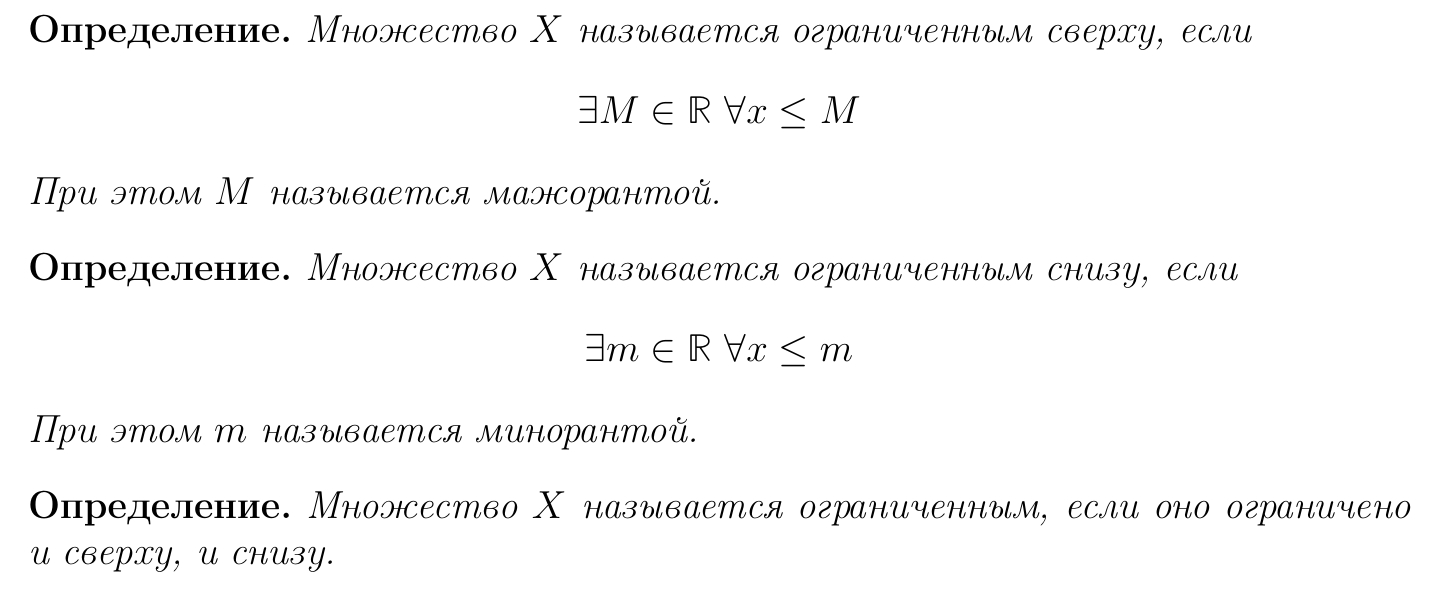
\includegraphics[width=17cm,height=6.98cm]{D0ADD0BAD0B7D0B0D0BCD0B5D0BDD0BED182D0B2D0B5D182D18B-img001.png}
 

\begin{equation*}
\begin{gathered}\boldsubformula{\mathit{\text{О}\text{п}\text{р}\text{е}\text{д}\text{е}\text{л}\text{е}\text{н}\text{и}\text{е}}\mathit{\text{в}\text{е}\text{р}\text{х}\text{н}\text{е}\text{й}}\mathit{\text{г}\text{р}\text{а}\text{н}\text{и}}\mathit{\text{м}\text{н}\text{о}\text{ж}\text{е}\text{с}\text{т}\text{в}\text{а}}}\\a=\mathit{su\text{р}}X\overset{\mathit{df}}{\Leftrightarrow
}(\forall x\in Xx\le a)\wedge (\forall a'\le a\exists x'\in Xx'\ge a)\overset{\mathit{df}}{\Leftrightarrow
}\genfrac{}{}{0pt}{0}{\left.1\right)\forall x\in Xx\le a}{\left.2\right)\forall \epsilon >0\exists x'\in Xa-\epsilon
<x'}\\\boldsubformula{\mathit{\text{О}\text{п}\text{р}\text{е}\text{д}\text{е}\text{л}\text{е}\text{н}\text{и}\text{е}}\mathit{\text{н}\text{и}\text{ж}\text{н}\text{е}\text{й}}\mathit{\text{г}\text{р}\text{а}\text{н}\text{и}}\mathit{\text{м}\text{н}\text{о}\text{ж}\text{е}\text{с}\text{т}\text{в}\text{а}}}\\a=\mathit{inf}X\overset{\mathit{df}}{\Leftrightarrow
}(\forall x\in Xx\ge a)\wedge (\forall a'\ge a\exists x'\in Xx'\le a)\overset{\mathit{df}}{\Leftrightarrow
}\genfrac{}{}{0pt}{0}{\left.1\right)\forall x\in Xx\ge a}{\left.2\right)\forall \epsilon >0\exists x'\in Xx<a+\epsilon
}\end{gathered}
\end{equation*}

\bigskip

  [Warning: Image ignored] % Unhandled or unsupported graphics:
%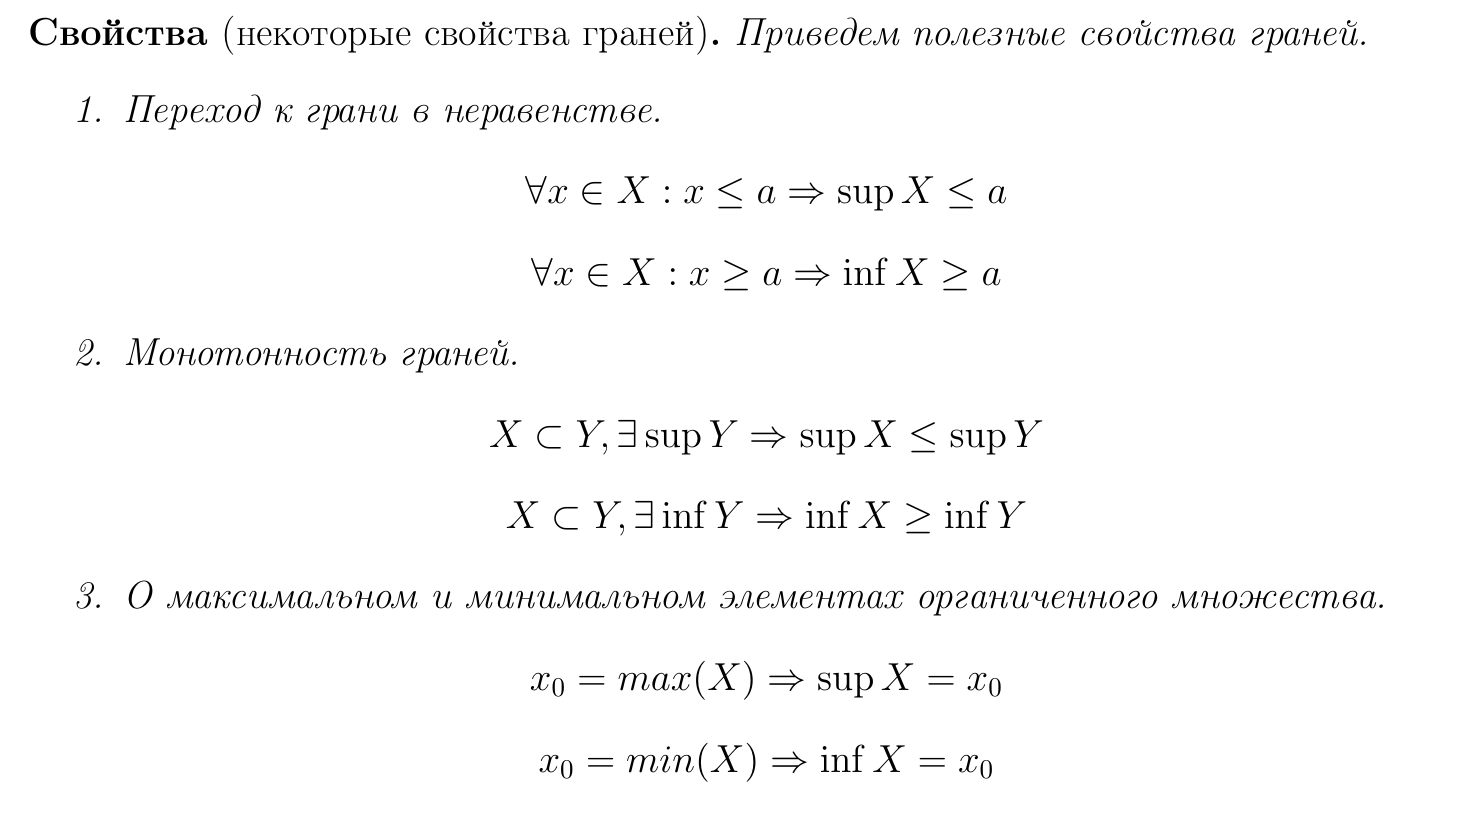
\includegraphics[width=17cm,height=9.449cm]{D0ADD0BAD0B7D0B0D0BCD0B5D0BDD0BED182D0B2D0B5D182D18B-img002.png}
 

\subsection{Теорема о существовании верхней грани.}
  [Warning: Image ignored] % Unhandled or unsupported graphics:
%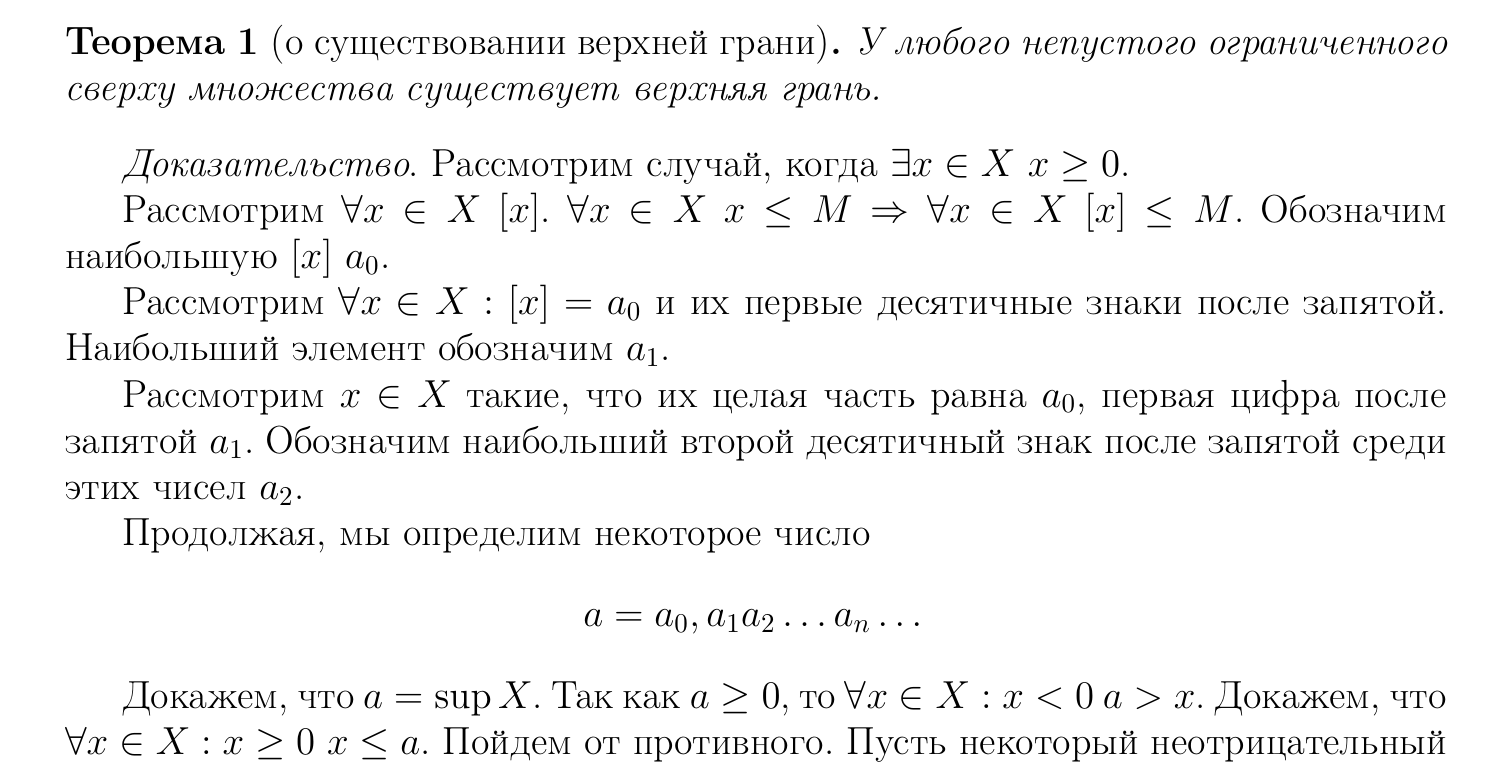
\includegraphics[width=17cm,height=8.83cm]{D0ADD0BAD0B7D0B0D0BCD0B5D0BDD0BED182D0B2D0B5D182D18B-img003.png}
 

  [Warning: Image ignored] % Unhandled or unsupported graphics:
%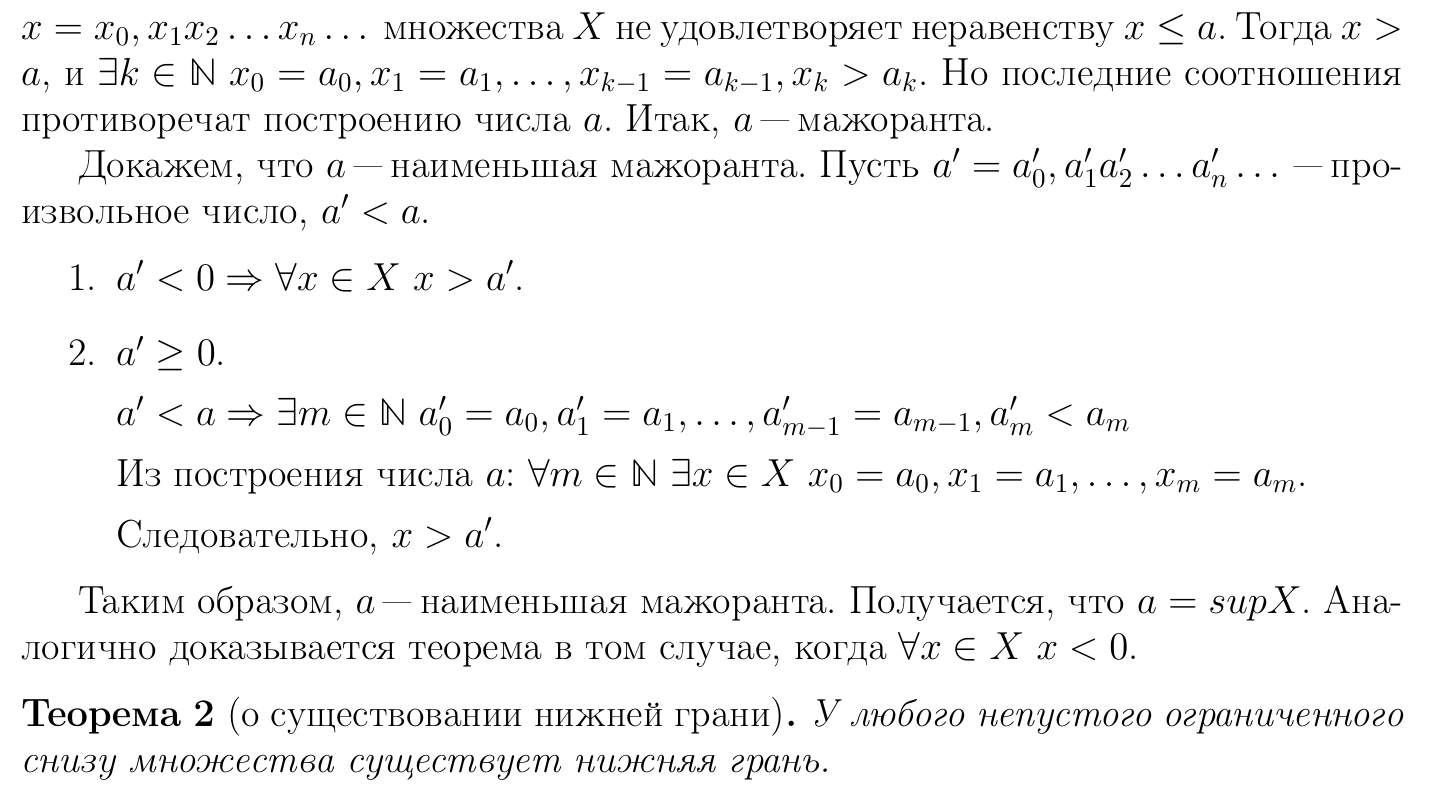
\includegraphics[width=17cm,height=9.283cm]{D0ADD0BAD0B7D0B0D0BCD0B5D0BDD0BED182D0B2D0B5D182D18B-img004.png}
 \newline
\newline


\subsection{Счетные множества и их свойства. }
  [Warning: Image ignored] % Unhandled or unsupported graphics:
%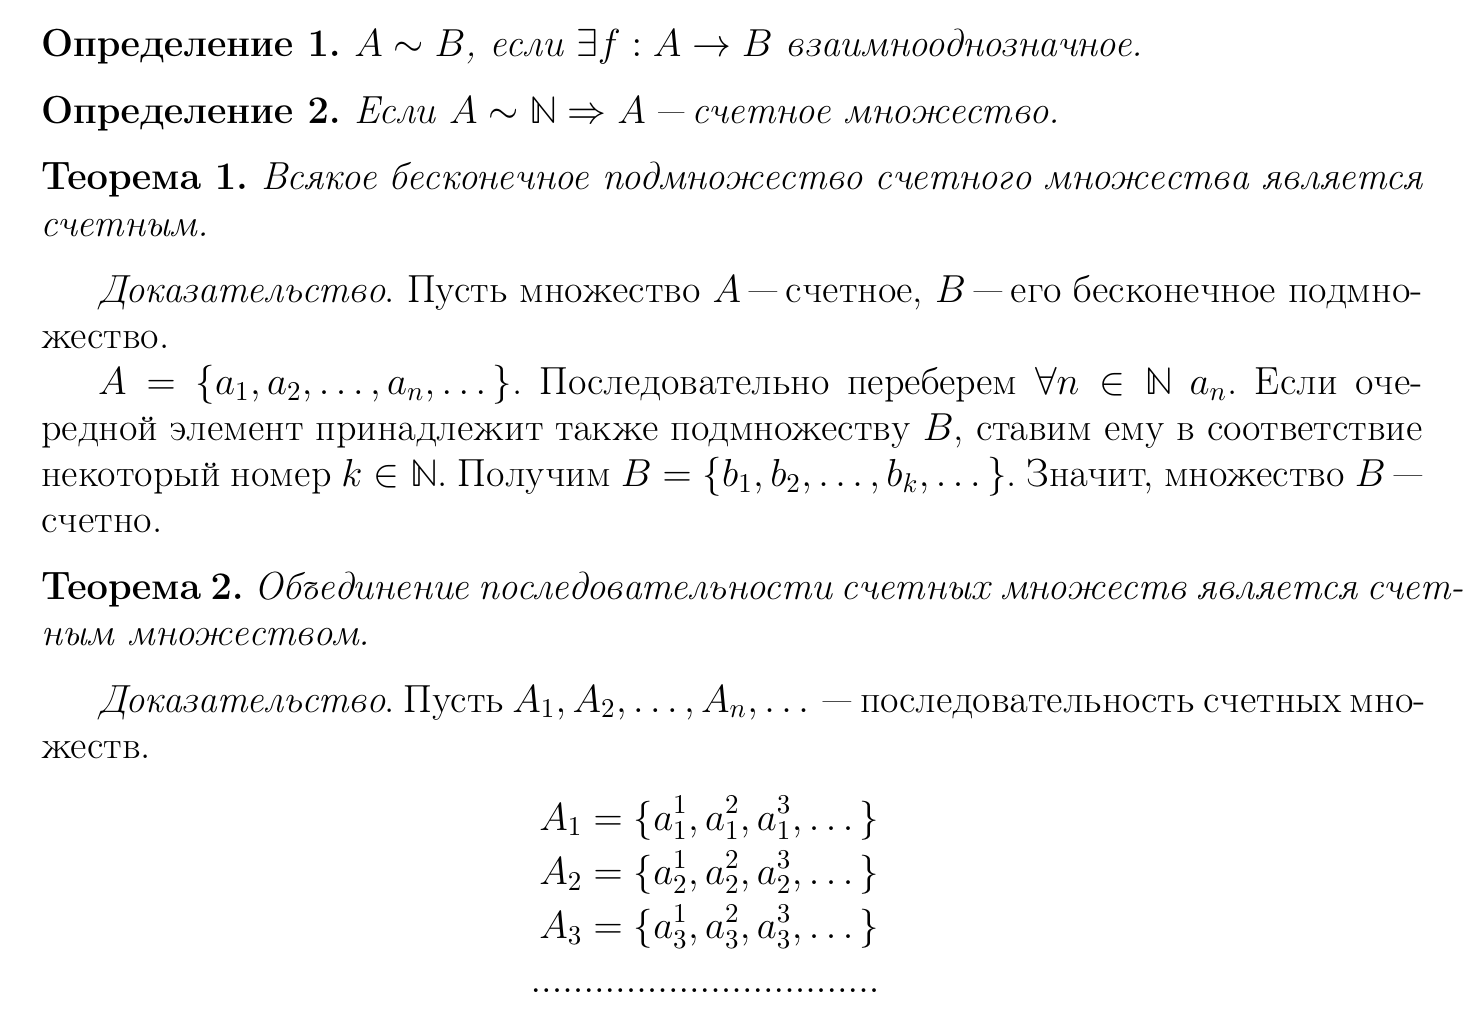
\includegraphics[width=17cm,height=11.703cm]{D0ADD0BAD0B7D0B0D0BCD0B5D0BDD0BED182D0B2D0B5D182D18B-img005.png}
 

  [Warning: Image ignored] % Unhandled or unsupported graphics:
%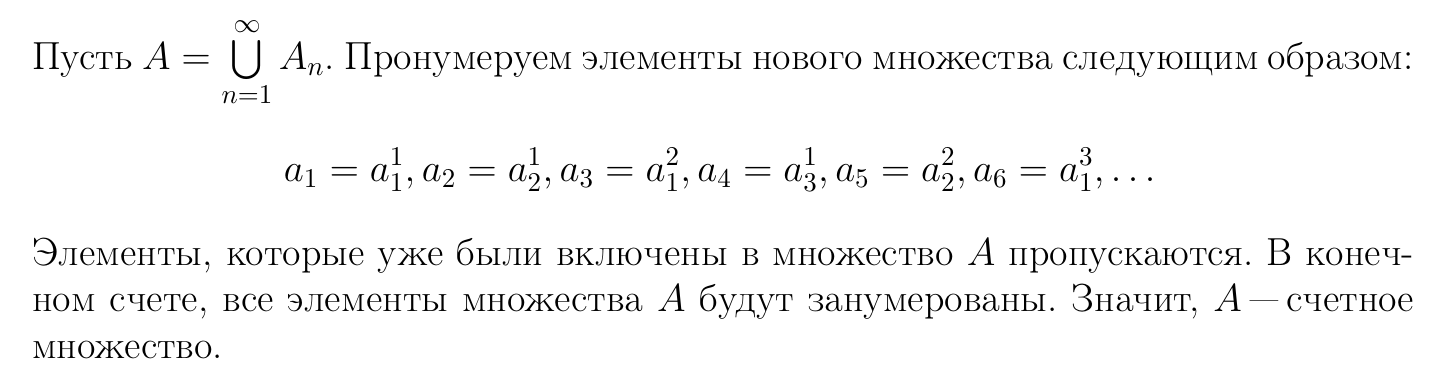
\includegraphics[width=17cm,height=4.526cm]{D0ADD0BAD0B7D0B0D0BCD0B5D0BDD0BED182D0B2D0B5D182D18B-img006.png}
 

\subsection{Теорема о несчетности интервала. Множества мощности континуум.}
  [Warning: Image ignored] % Unhandled or unsupported graphics:
%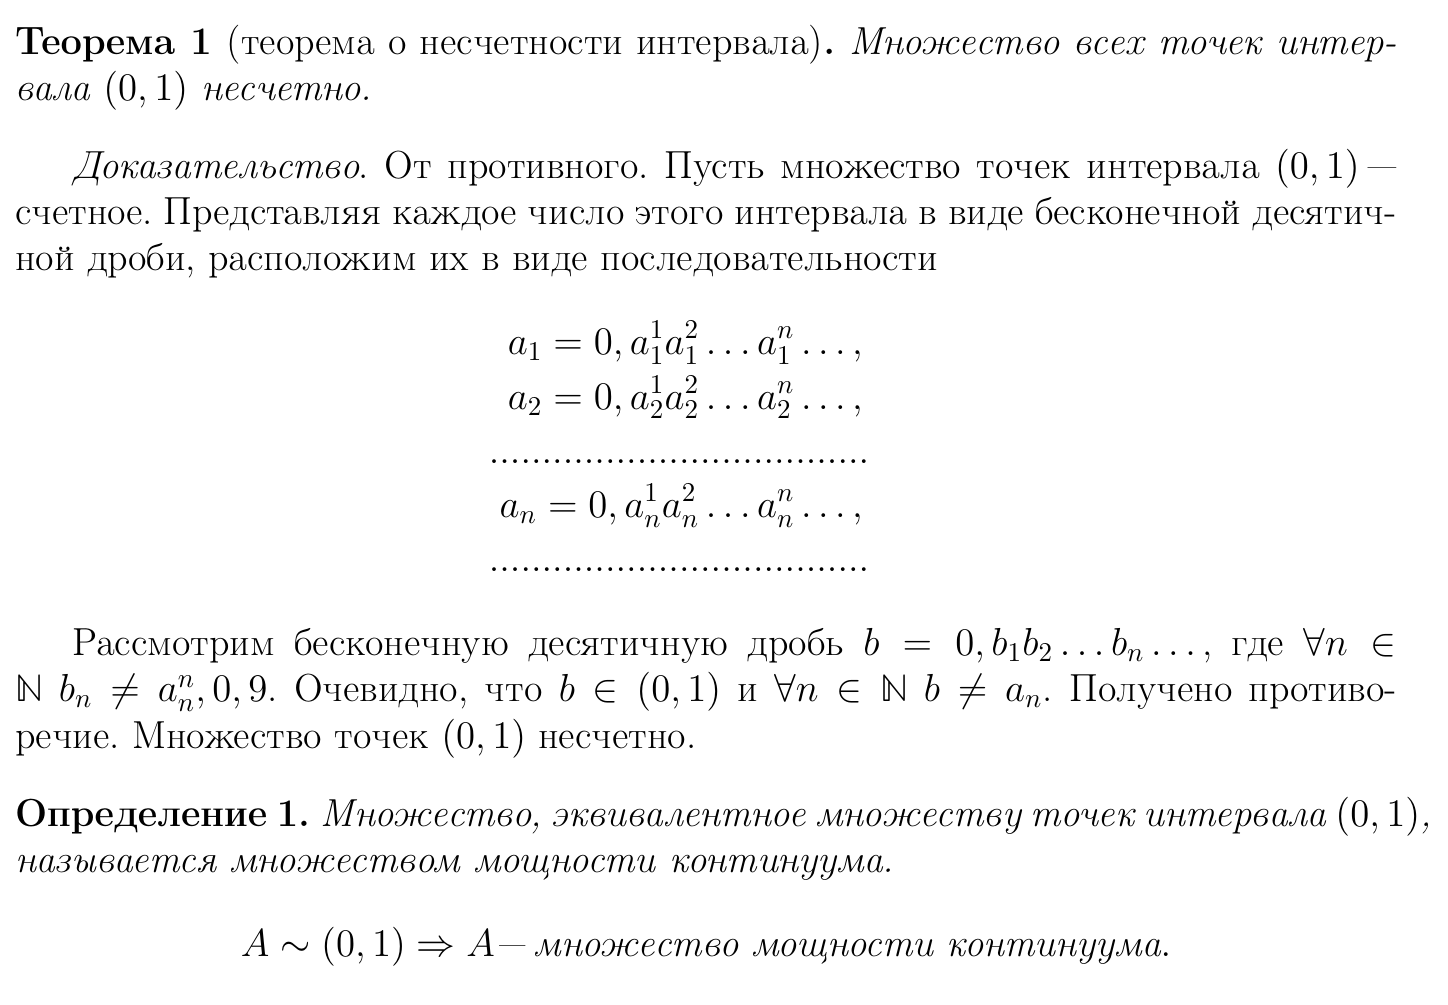
\includegraphics[width=17cm,height=11.799cm]{D0ADD0BAD0B7D0B0D0BCD0B5D0BDD0BED182D0B2D0B5D182D18B-img007.png}
 

\subsection{Ограниченные последовательности. Достаточное условие ограниченности последовательности.}
\begin{equation*}
\begin{gathered}\boldsubformula{\mathit{\text{О}\text{п}\text{р}\text{е}\text{д}\text{е}\text{л}\text{е}\text{н}\text{и}\text{е}}\mathit{\text{п}\text{о}\text{с}\text{л}\text{е}\text{д}\text{о}\text{в}\text{а}\text{т}\text{е}\text{л}\text{ь}\text{н}\text{о}\text{с}\text{т}\text{и}}}\\(x_n)\overset{\mathit{df}}{\Leftrightarrow
}f:\mathbb{N}->\mathbb{R}\\{}\\(x_n)-\mathit{\text{о}\text{г}\text{р}.}\mathit{\text{с}\text{в}\text{е}\text{р}\text{х}\text{у}}\overset{\mathit{df}}{\Leftrightarrow
}\exists M\in \mathbb{R}\forall n\in \mathbb{N}x_n\le
M\\(x_n)-\mathit{\text{о}\text{г}\text{р}.}\mathit{\text{с}\text{н}\text{и}\text{з}\text{у}}\overset{\mathit{df}}{\Leftrightarrow
}\exists m\in \mathbb{R}\forall n\in \mathbb{N}x_n\ge M\\(x_n)=O(1)\overset{\mathit{df}}{\Leftrightarrow }\exists
M>0\forall n\in \mathbb{N}|x_n|\le M\\{}\end{gathered}
\end{equation*}
  [Warning: Image ignored] % Unhandled or unsupported graphics:
%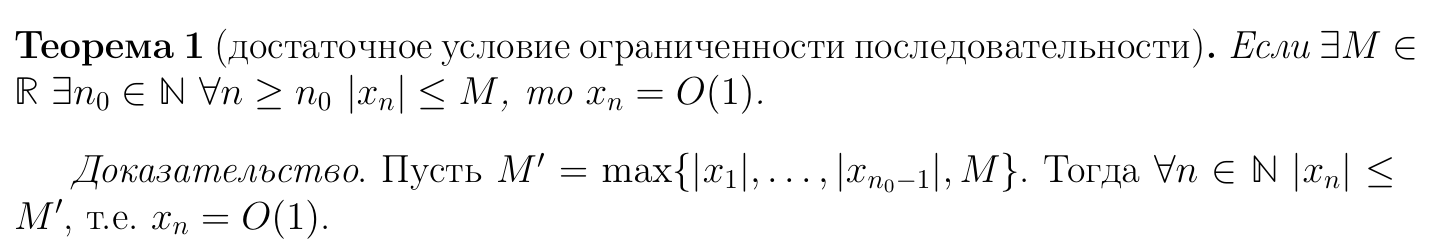
\includegraphics[width=17cm,height=2.914cm]{D0ADD0BAD0B7D0B0D0BCD0B5D0BDD0BED182D0B2D0B5D182D18B-img008.png}
 

\subsection{Бесконечно малые последовательности. Теорема об арифметических действиях над бесконечно малыми
последовательностями. }
  [Warning: Image ignored] % Unhandled or unsupported graphics:
%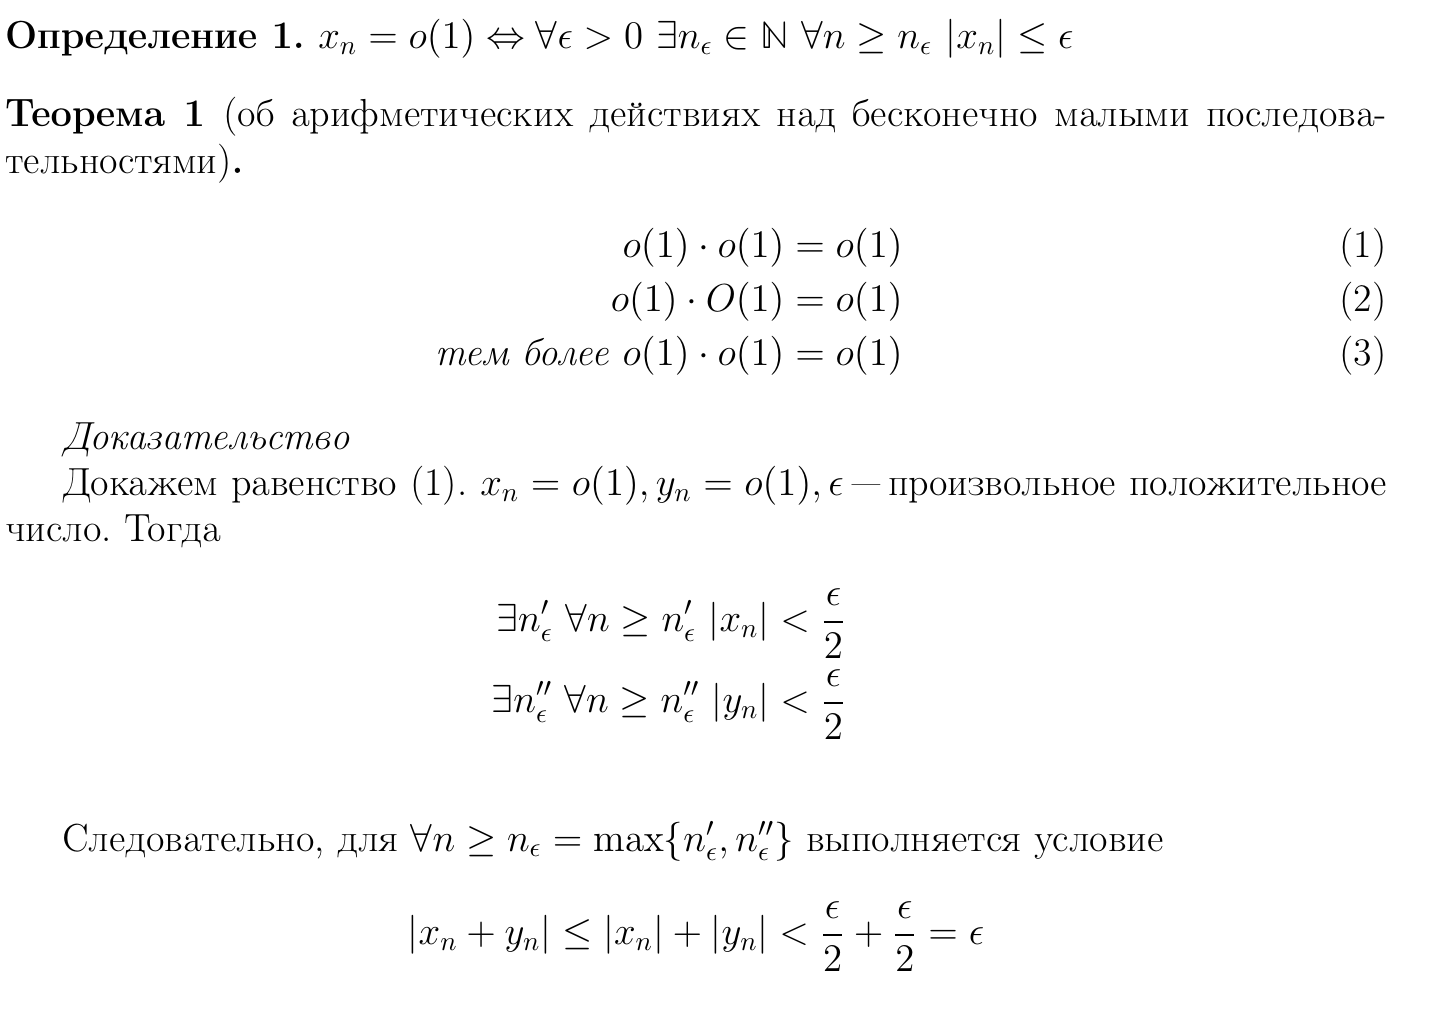
\includegraphics[width=17cm,height=11.959cm]{D0ADD0BAD0B7D0B0D0BCD0B5D0BDD0BED182D0B2D0B5D182D18B-img009.png}
 

  [Warning: Image ignored] % Unhandled or unsupported graphics:
%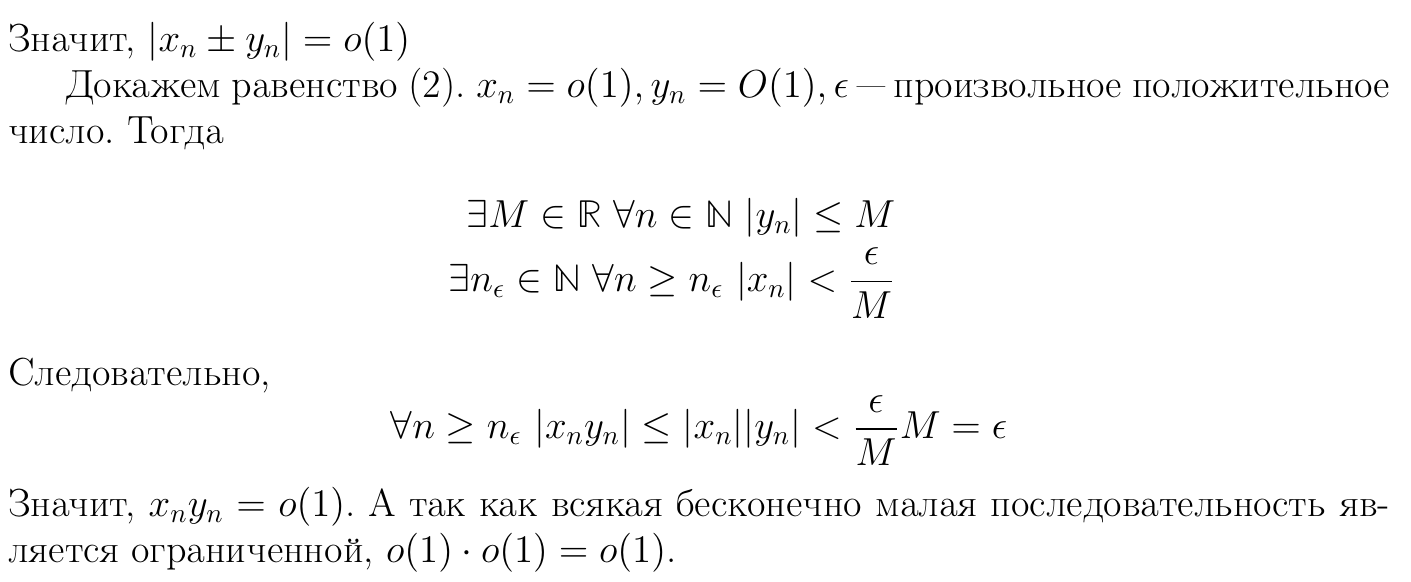
\includegraphics[width=17cm,height=7.011cm]{D0ADD0BAD0B7D0B0D0BCD0B5D0BDD0BED182D0B2D0B5D182D18B-img010.png}
 

\subsection{Бесконечно большие последовательности, их связь с бесконечно малыми.}
\begin{equation*}
\begin{gathered}\lim _{n->\infty }x_n=+\infty \overset{\mathit{df}}{\Leftrightarrow }\forall M>0\exists n_M\in
\mathbb{N}\forall n\ge n_Mx_n>M\\\lim _{n->\infty }x_n=-\infty \overset{\mathit{df}}{\Leftrightarrow }\forall
M>0\exists n_M\in \mathbb{N}\forall n\ge n_Mx_n<-M\\\lim _{n->\infty }x_n=\infty \overset{\mathit{df}}{\Leftrightarrow
}\forall M>0\exists n_M\in \mathbb{N}\forall n\ge n_M|x_n|>M\end{gathered}
\end{equation*}
  [Warning: Image ignored] % Unhandled or unsupported graphics:
%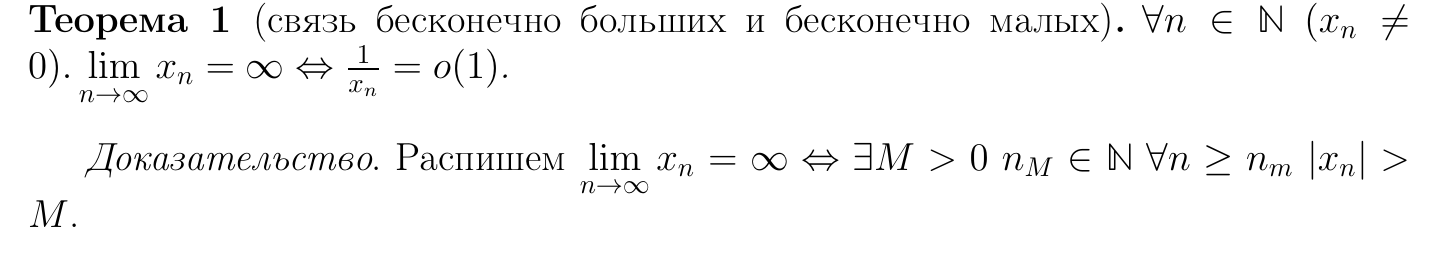
\includegraphics[width=17cm,height=3.066cm]{D0ADD0BAD0B7D0B0D0BCD0B5D0BDD0BED182D0B2D0B5D182D18B-img011.png}
 

  [Warning: Image ignored] % Unhandled or unsupported graphics:
%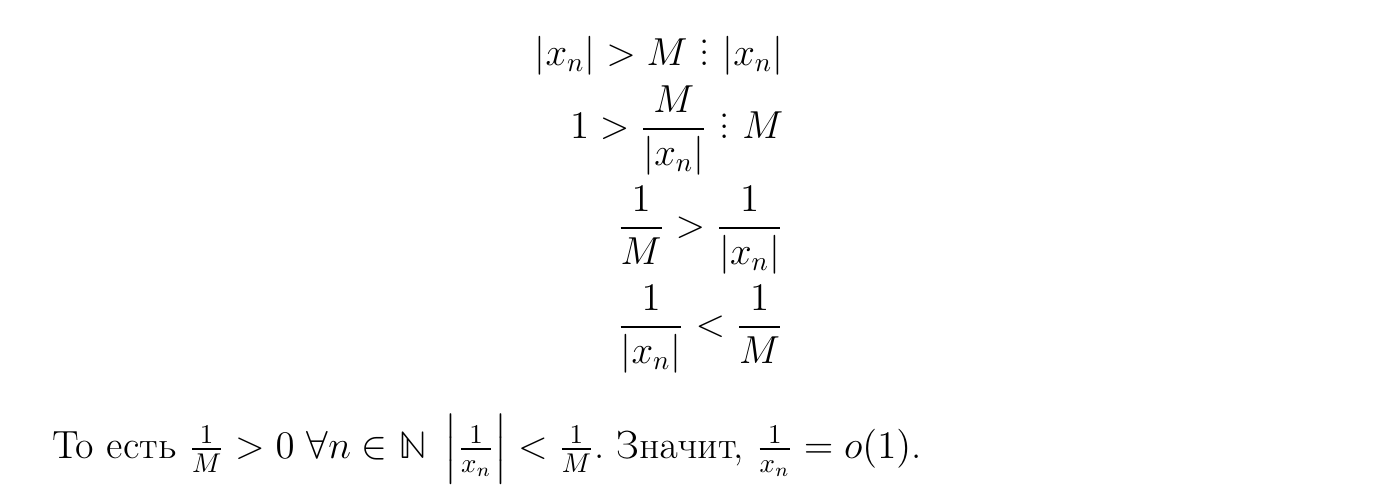
\includegraphics[width=17cm,height=6.068cm]{D0ADD0BAD0B7D0B0D0BCD0B5D0BDD0BED182D0B2D0B5D182D18B-img012.png}
 

\subsection{Предел последовательности. Теорема о единственности предела.}
  [Warning: Image ignored] % Unhandled or unsupported graphics:
%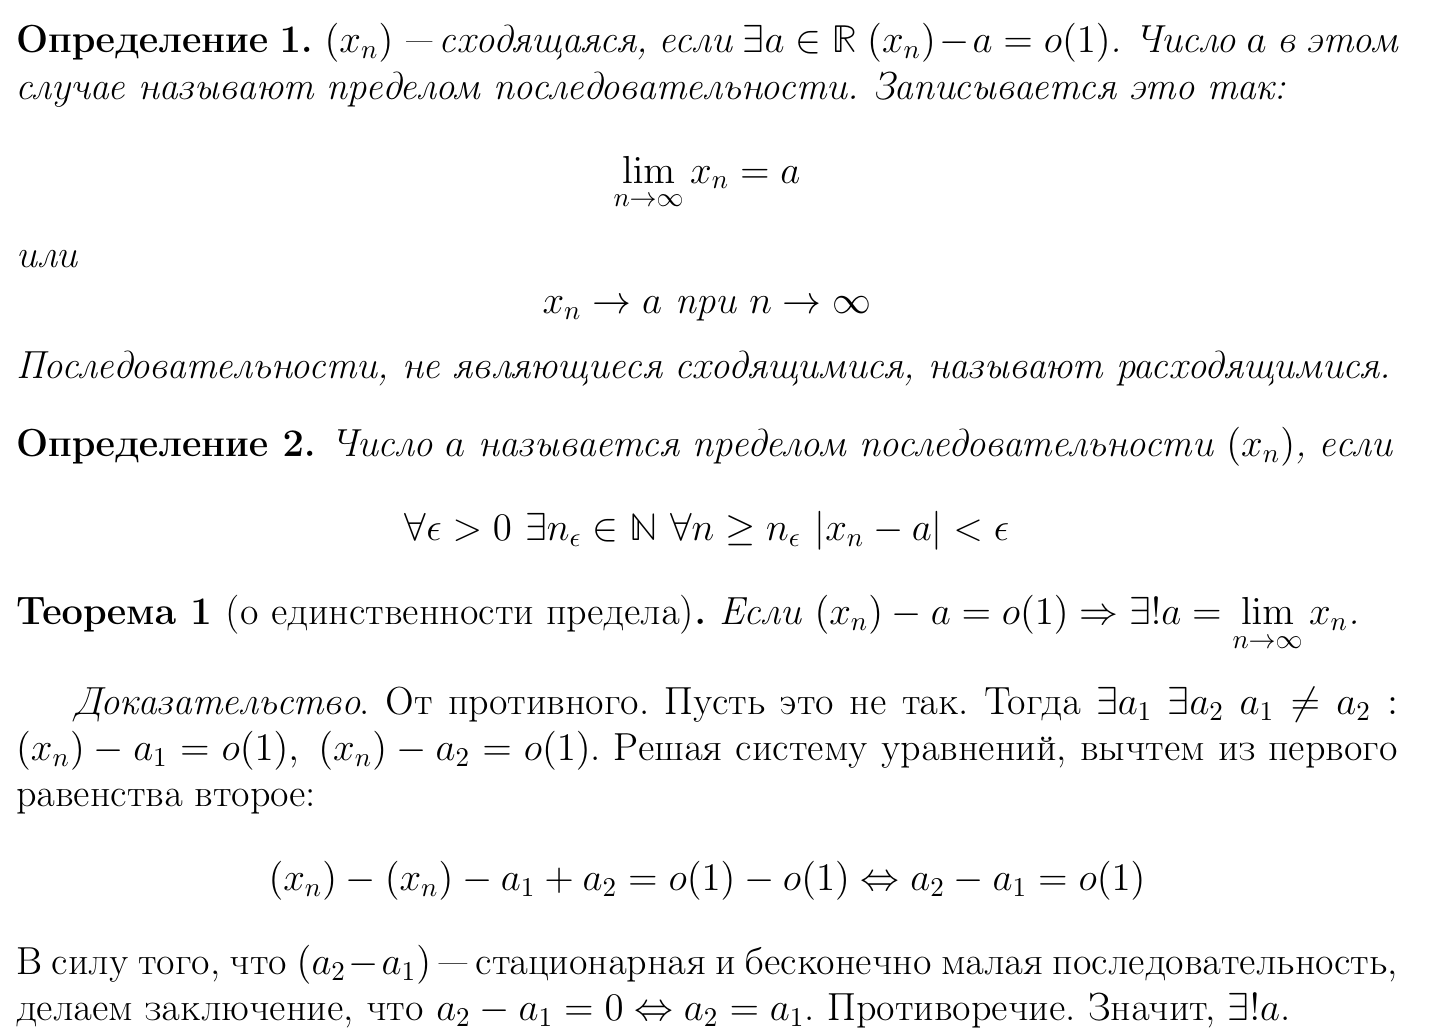
\includegraphics[width=17cm,height=12.204cm]{D0ADD0BAD0B7D0B0D0BCD0B5D0BDD0BED182D0B2D0B5D182D18B-img013.png}
 

\subsection{Ограниченность сходящейся последовательности.}
  [Warning: Image ignored] % Unhandled or unsupported graphics:
%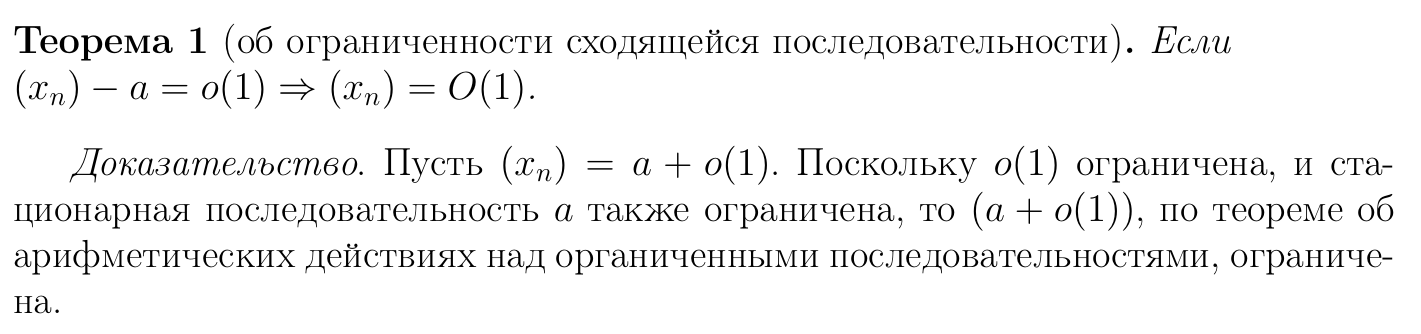
\includegraphics[width=17cm,height=3.995cm]{D0ADD0BAD0B7D0B0D0BCD0B5D0BDD0BED182D0B2D0B5D182D18B-img014.png}
 

\subsection{Порядковые свойства предела. Переход к пределу в неравенствах.}
  [Warning: Image ignored] % Unhandled or unsupported graphics:
%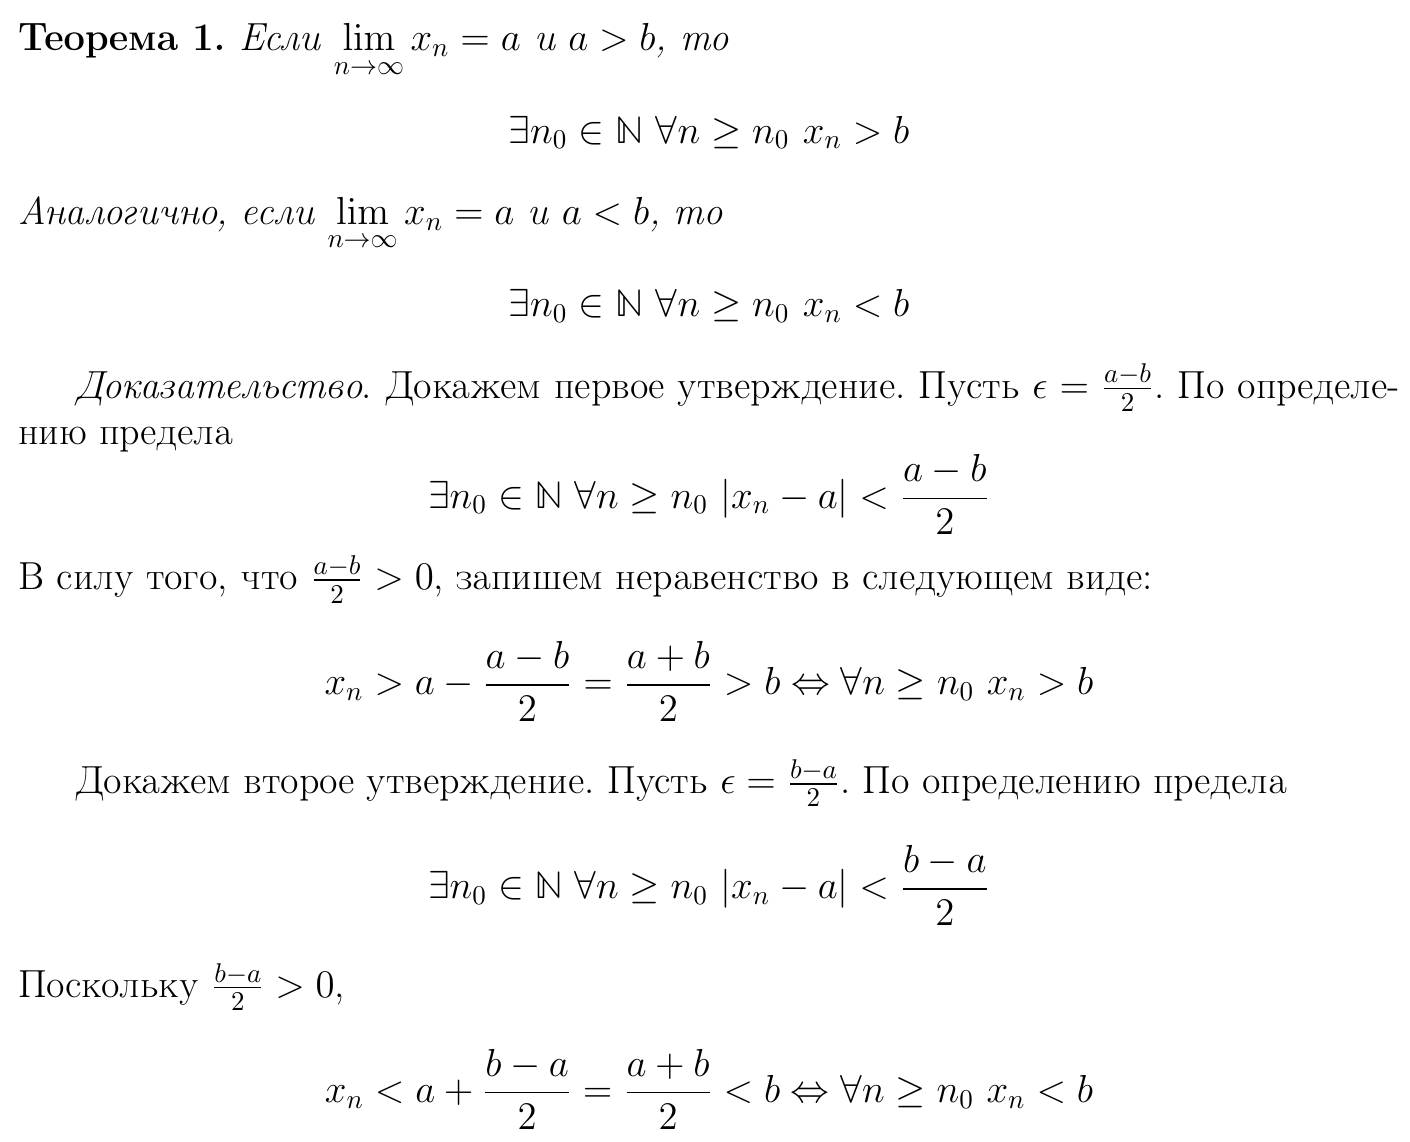
\includegraphics[width=17cm,height=13.767cm]{D0ADD0BAD0B7D0B0D0BCD0B5D0BDD0BED182D0B2D0B5D182D18B-img015.png}
 

  [Warning: Image ignored] % Unhandled or unsupported graphics:
%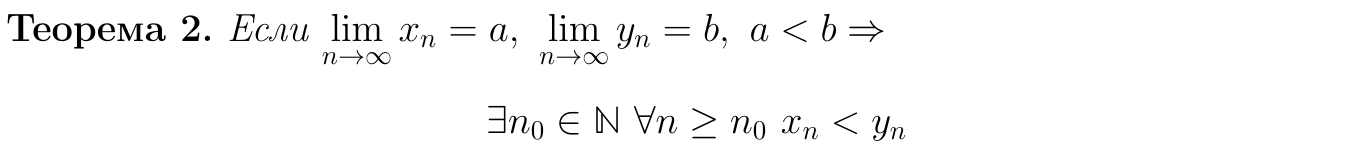
\includegraphics[width=17cm,height=2.02cm]{D0ADD0BAD0B7D0B0D0BCD0B5D0BDD0BED182D0B2D0B5D182D18B-img016.png}
 

  [Warning: Image ignored] % Unhandled or unsupported graphics:
%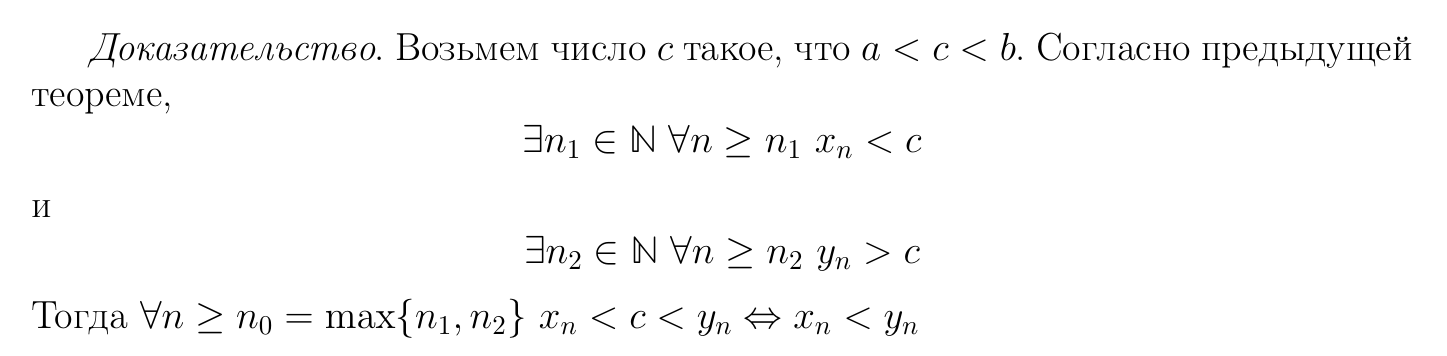
\includegraphics[width=17cm,height=4.182cm]{D0ADD0BAD0B7D0B0D0BCD0B5D0BDD0BED182D0B2D0B5D182D18B-img017.png}
 

  [Warning: Image ignored] % Unhandled or unsupported graphics:
%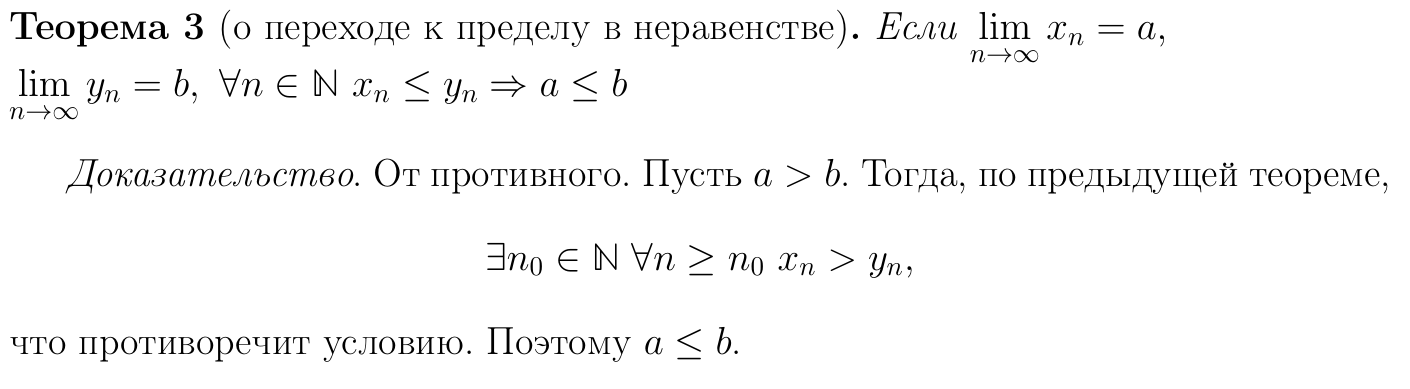
\includegraphics[width=17cm,height=4.688cm]{D0ADD0BAD0B7D0B0D0BCD0B5D0BDD0BED182D0B2D0B5D182D18B-img018.png}
 

\subsection{Порядковый признак существования предела последовательности.}
  [Warning: Image ignored] % Unhandled or unsupported graphics:
%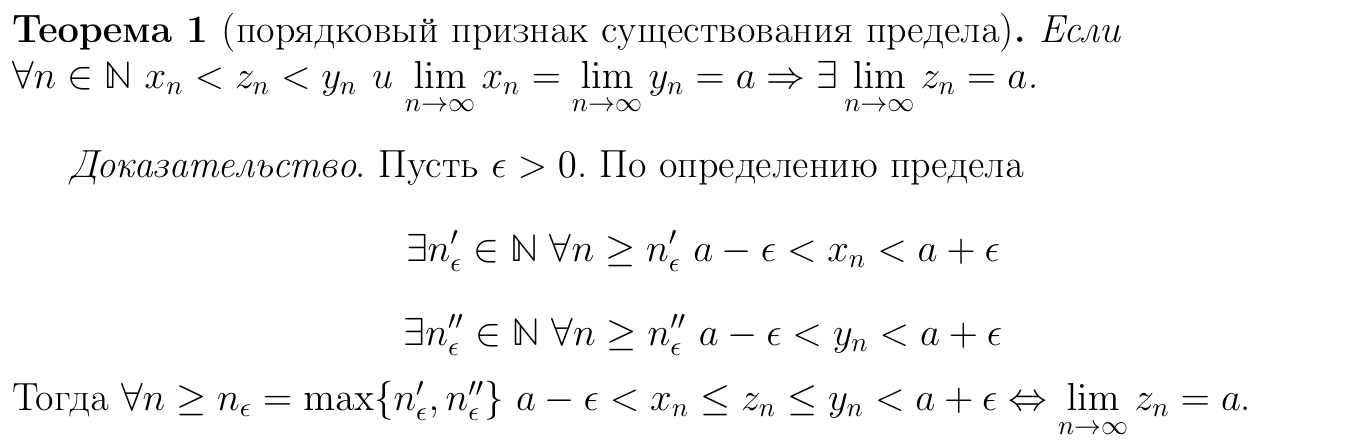
\includegraphics[width=17cm,height=5.607cm]{D0ADD0BAD0B7D0B0D0BCD0B5D0BDD0BED182D0B2D0B5D182D18B-img019.png}
 

\subsection{Арифметические свойства предела последовательности.}
  [Warning: Image ignored] % Unhandled or unsupported graphics:
%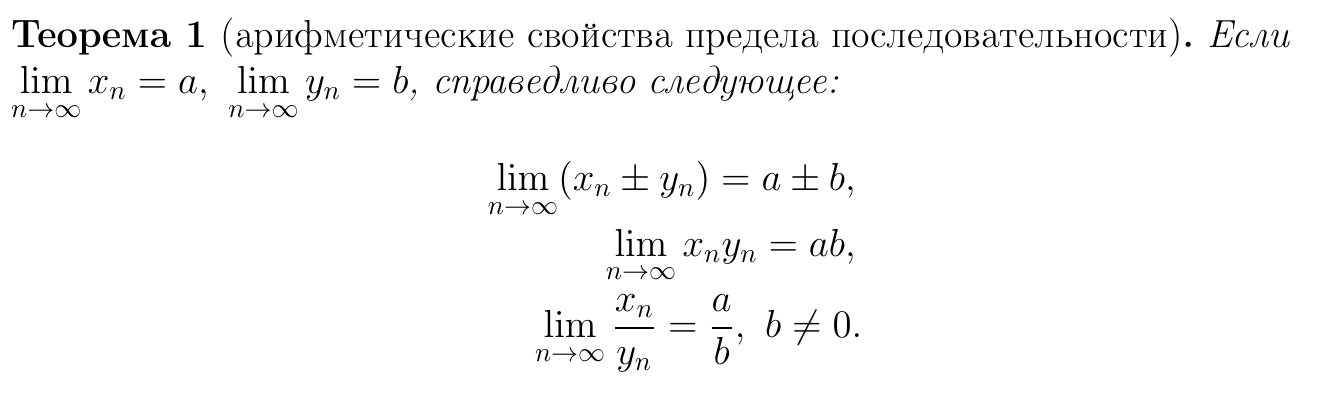
\includegraphics[width=17cm,height=5.144cm]{D0ADD0BAD0B7D0B0D0BCD0B5D0BDD0BED182D0B2D0B5D182D18B-img020.png}
 

  [Warning: Image ignored] % Unhandled or unsupported graphics:
%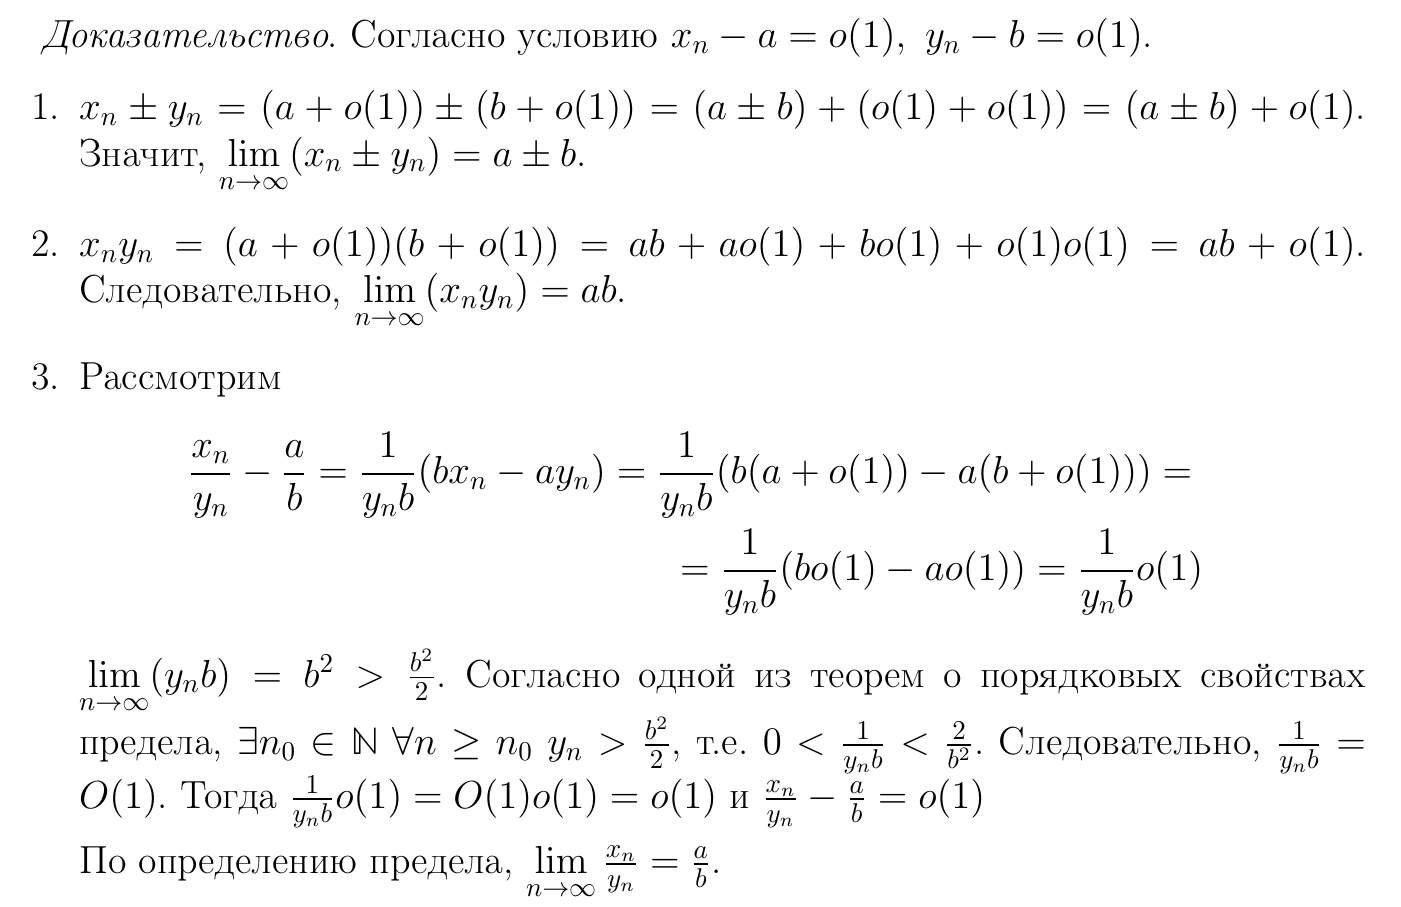
\includegraphics[width=17cm,height=11.005cm]{D0ADD0BAD0B7D0B0D0BCD0B5D0BDD0BED182D0B2D0B5D182D18B-img021.png}
 

\subsection{Монотонные последовательности. Теорема Вейерштрасса о монотонных последовательностях.}
  [Warning: Image ignored] % Unhandled or unsupported graphics:
%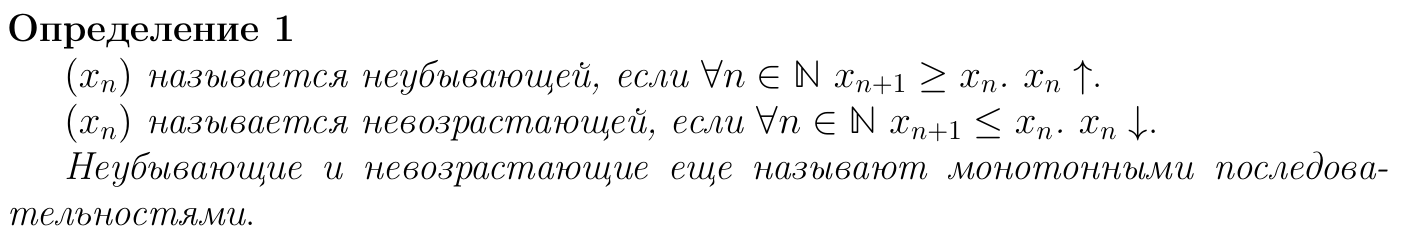
\includegraphics[width=17cm,height=3.007cm]{D0ADD0BAD0B7D0B0D0BCD0B5D0BDD0BED182D0B2D0B5D182D18B-img022.png}
 

  [Warning: Image ignored] % Unhandled or unsupported graphics:
%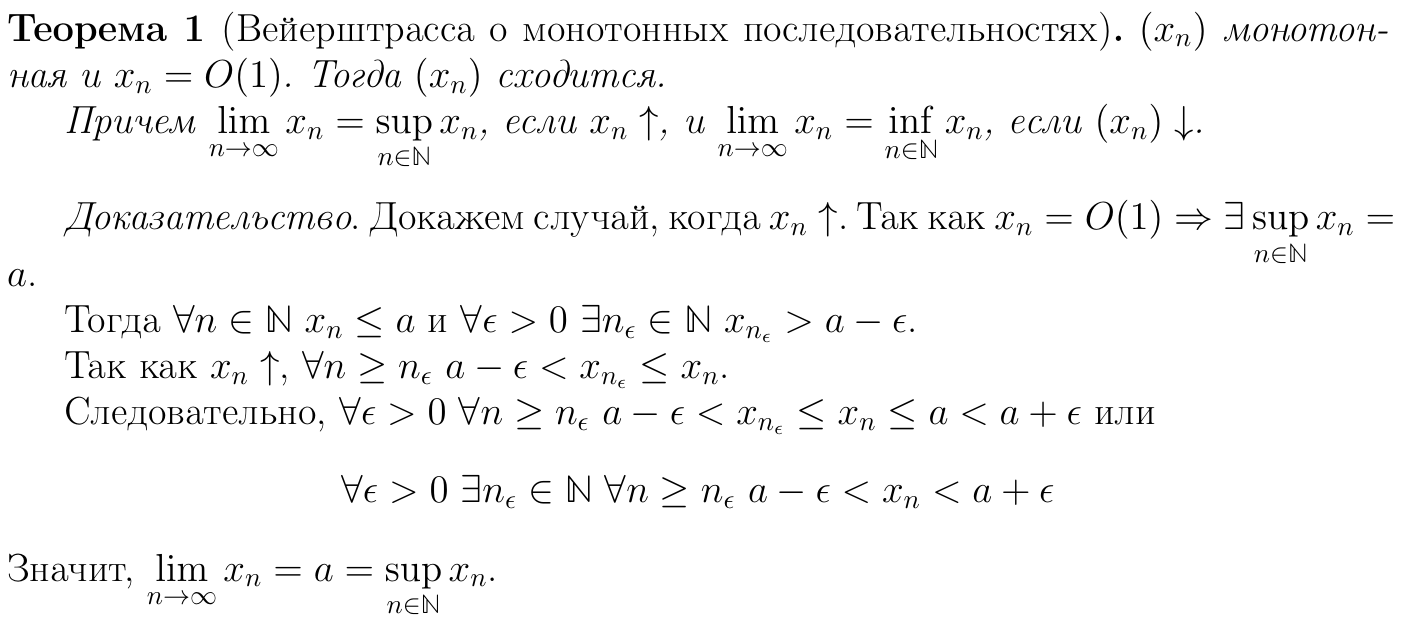
\includegraphics[width=17cm,height=7.535cm]{D0ADD0BAD0B7D0B0D0BCD0B5D0BDD0BED182D0B2D0B5D182D18B-img023.png}
 

  [Warning: Image ignored] % Unhandled or unsupported graphics:
%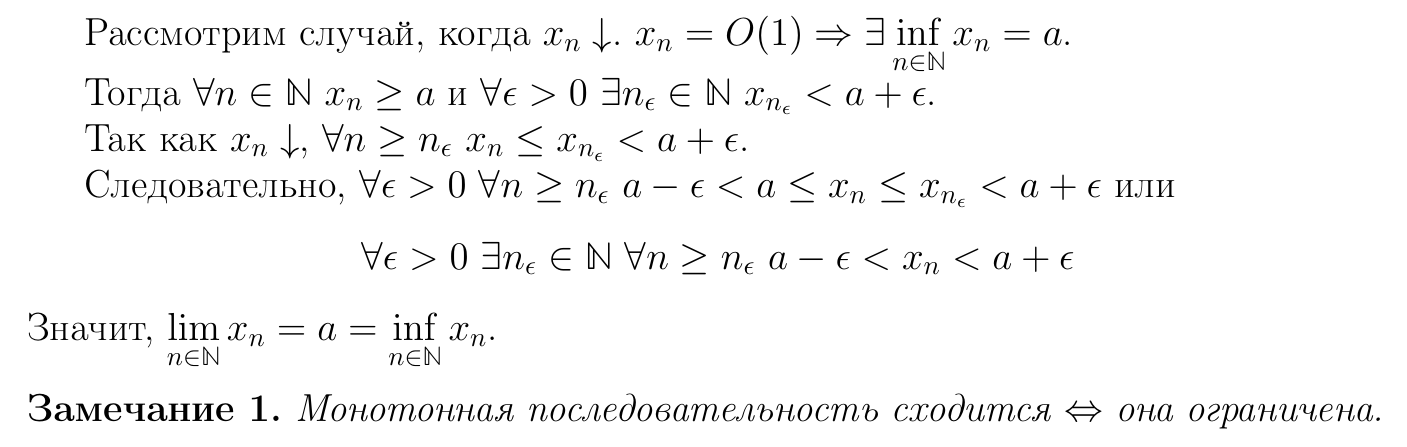
\includegraphics[width=17cm,height=5.399cm]{D0ADD0BAD0B7D0B0D0BCD0B5D0BDD0BED182D0B2D0B5D182D18B-img024.png}
 

\subsection{Лемма о вложенных отрезках.}
  [Warning: Image ignored] % Unhandled or unsupported graphics:
%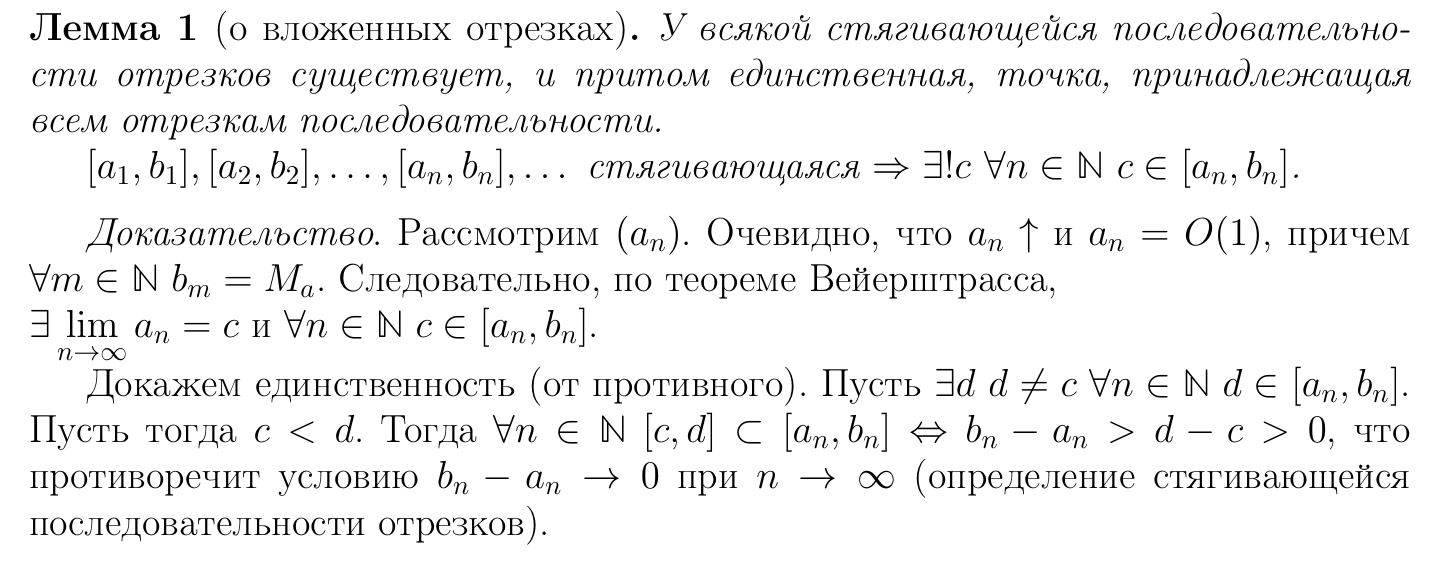
\includegraphics[width=17cm,height=6.66cm]{D0ADD0BAD0B7D0B0D0BCD0B5D0BDD0BED182D0B2D0B5D182D18B-img025.png}
 

\subsection{Подпоследовательности и частичные пределы последовательности. Теорема о подпоследовательностях сходящейся
последовательности. }
  [Warning: Image ignored] % Unhandled or unsupported graphics:
%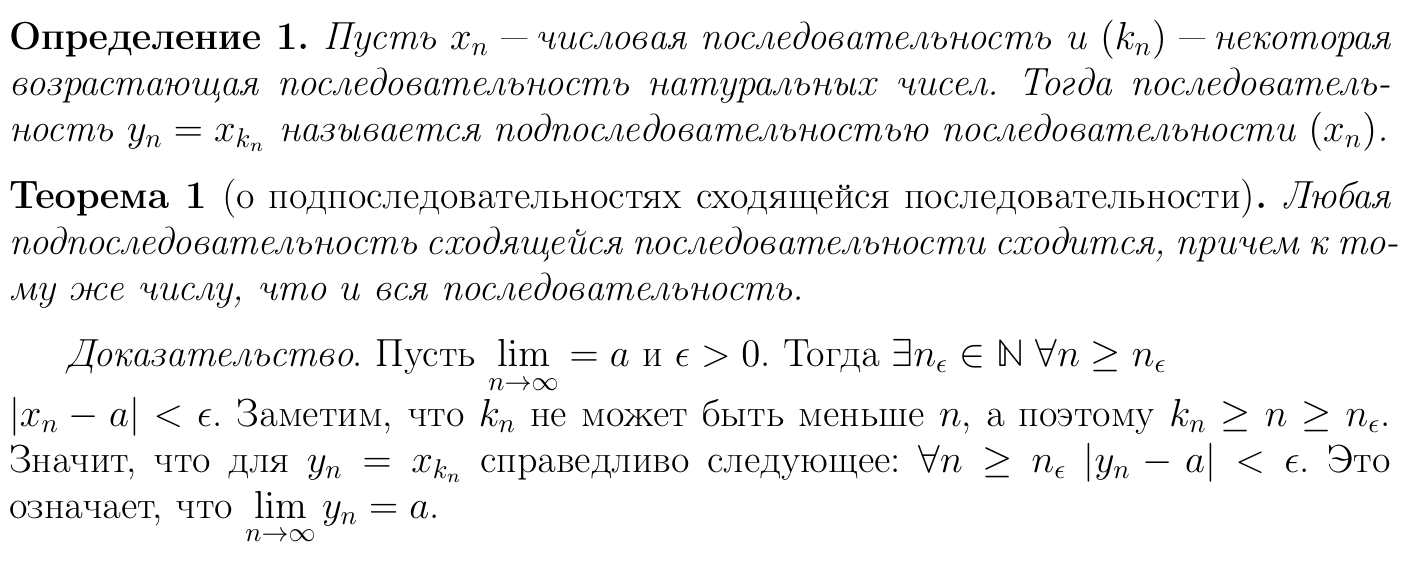
\includegraphics[width=17cm,height=6.821cm]{D0ADD0BAD0B7D0B0D0BCD0B5D0BDD0BED182D0B2D0B5D182D18B-img026.png}
 

\subsection{Верхний и нижний пределы последовательности. Корректность определения. }
  [Warning: Image ignored] % Unhandled or unsupported graphics:
%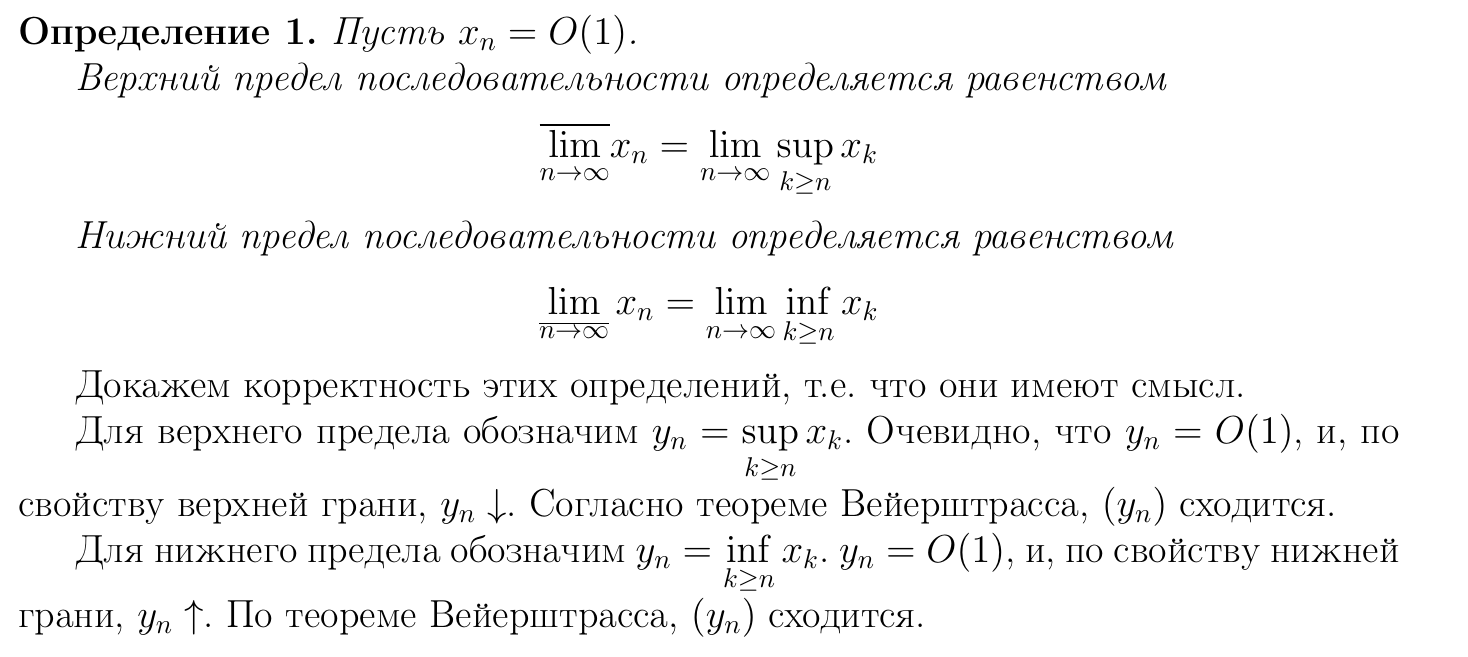
\includegraphics[width=17cm,height=7.608cm]{D0ADD0BAD0B7D0B0D0BCD0B5D0BDD0BED182D0B2D0B5D182D18B-img027.png}
 

\subsection{Свойства верхнего и нижнего пределов.}
  [Warning: Image ignored] % Unhandled or unsupported graphics:
%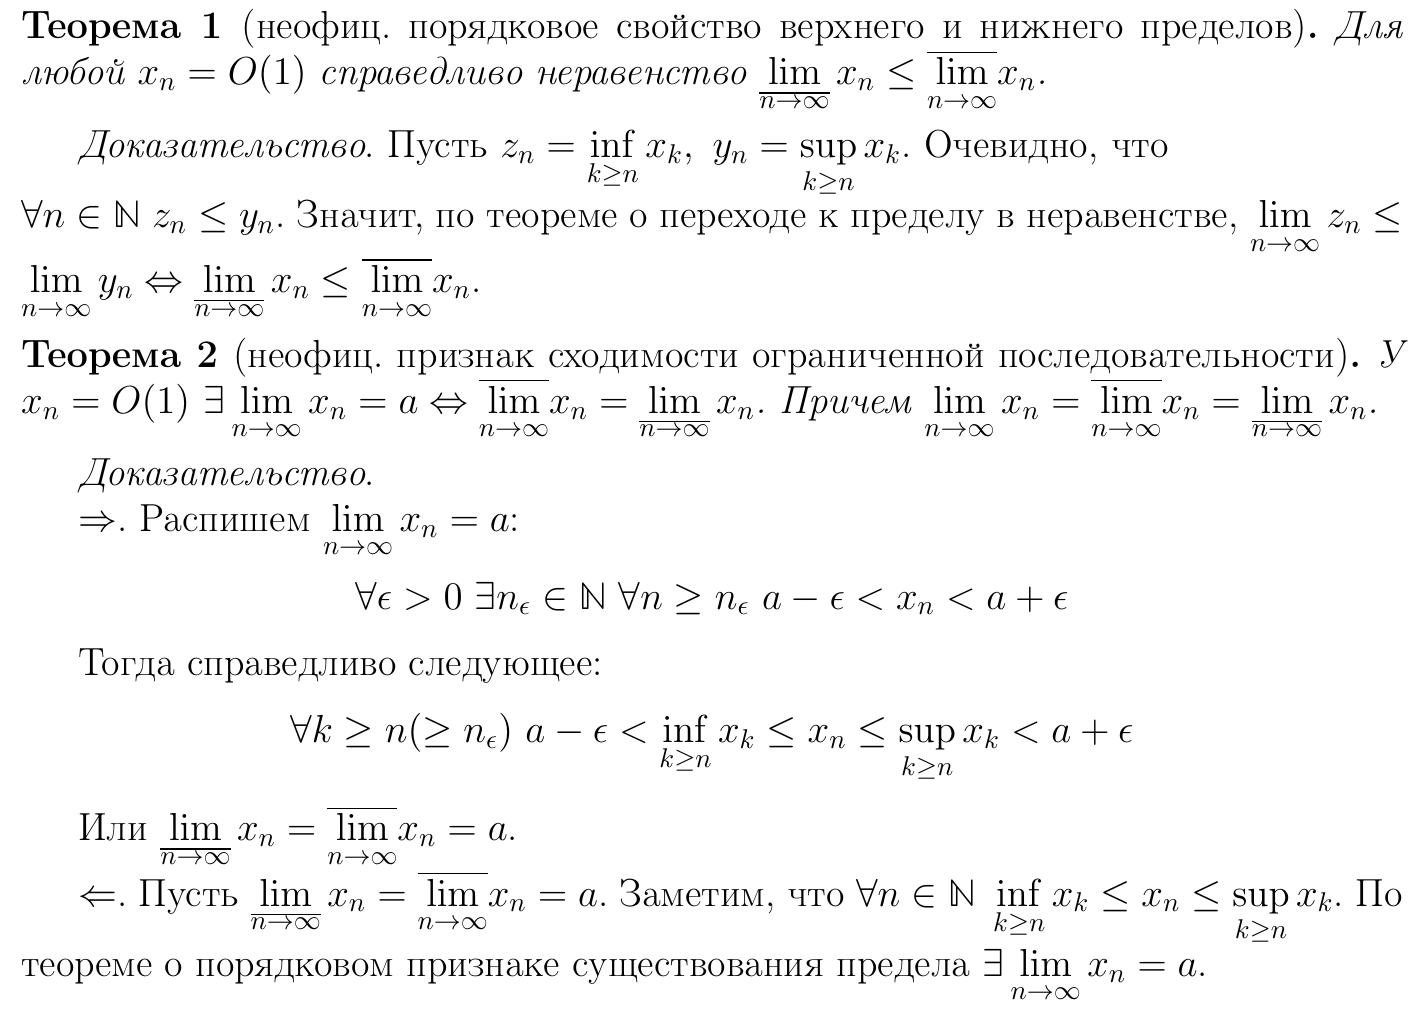
\includegraphics[width=17cm,height=12.012cm]{D0ADD0BAD0B7D0B0D0BCD0B5D0BDD0BED182D0B2D0B5D182D18B-img028.png}
 

\subsection[Теорема Больцано{}-Вейерштрасса.]{Теорема Больцано-Вейерштрасса.}
  [Warning: Image ignored] % Unhandled or unsupported graphics:
%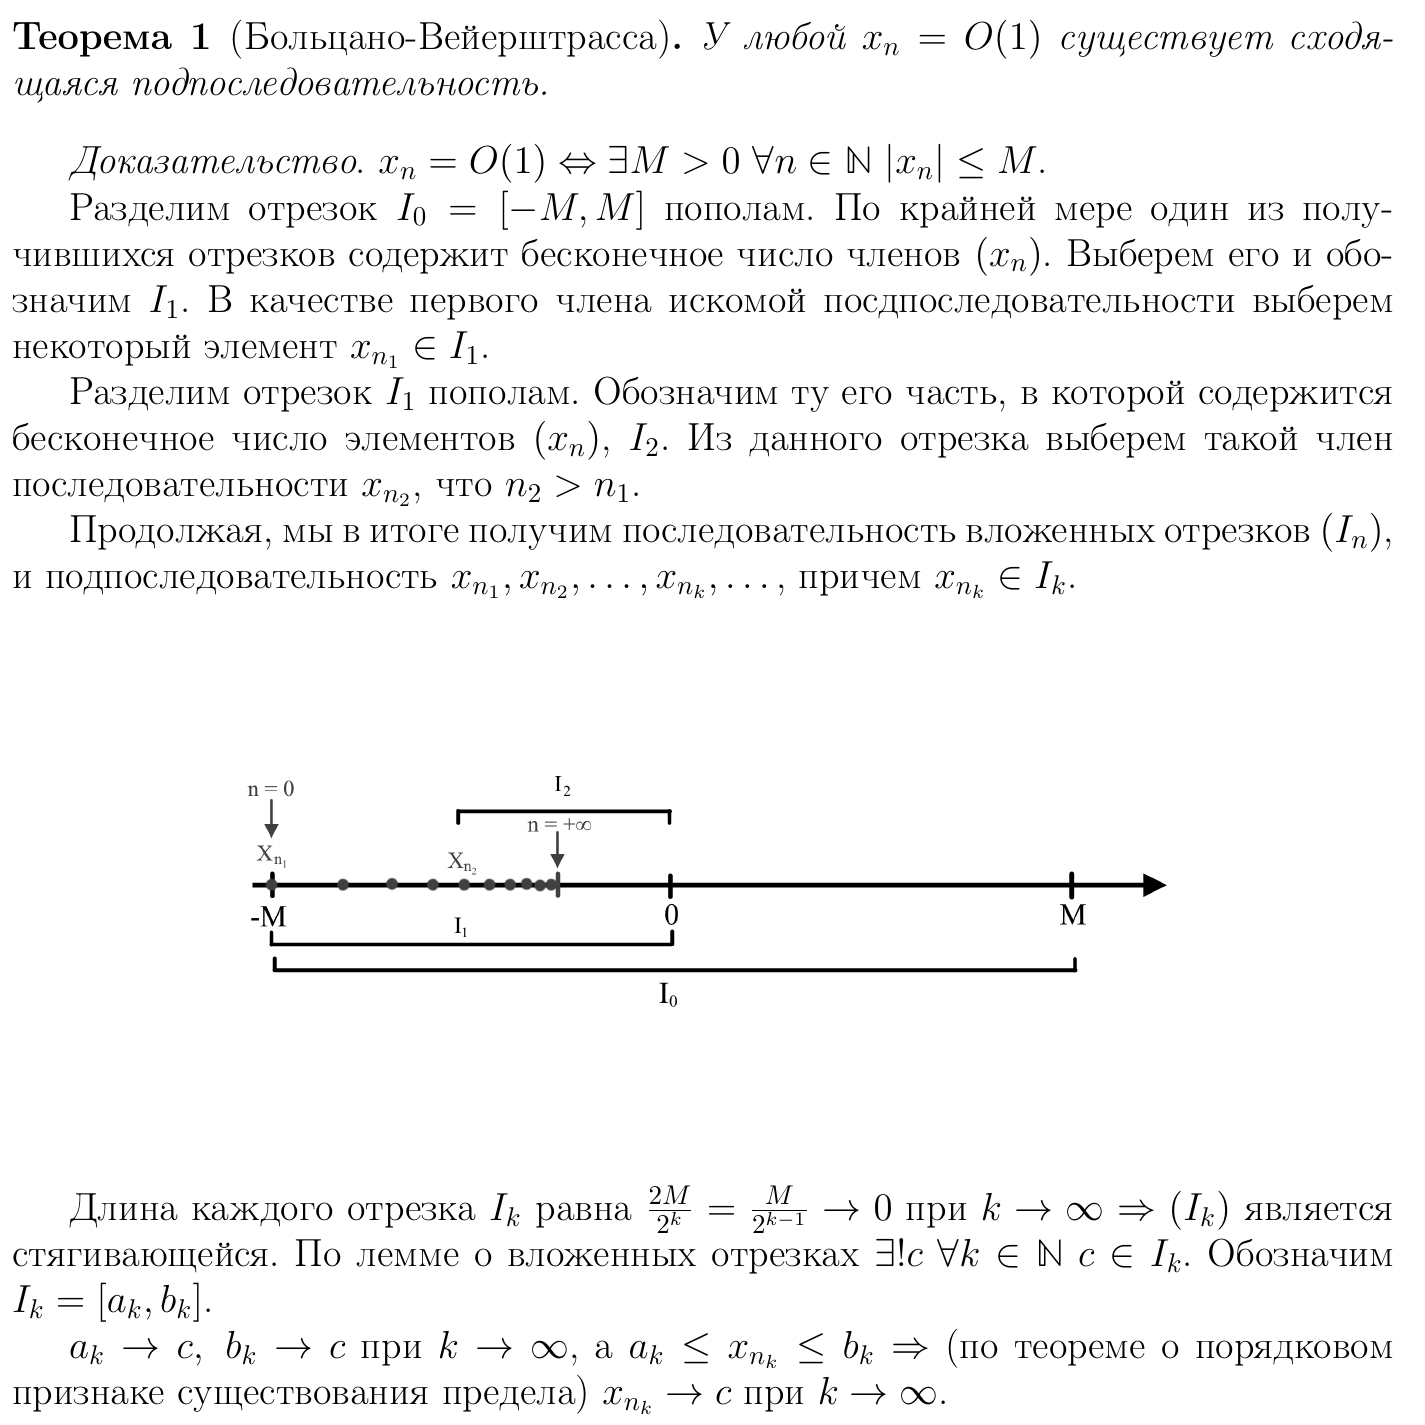
\includegraphics[width=17cm,height=17cm]{D0ADD0BAD0B7D0B0D0BCD0B5D0BDD0BED182D0B2D0B5D182D18B-img029.png}
 

\subsection{Фундаментальные последовательности. Теорема об ограниченности фундаментальной последовательности. \ }
  [Warning: Image ignored] % Unhandled or unsupported graphics:
%
\includegraphics[width=17cm,height=2.076cm]{D0ADD0BAD0B7D0B0D0BCD0B5D0BDD0BED182D0B2D0B5D182D18B-img030.png}
 

  [Warning: Image ignored] % Unhandled or unsupported graphics:
%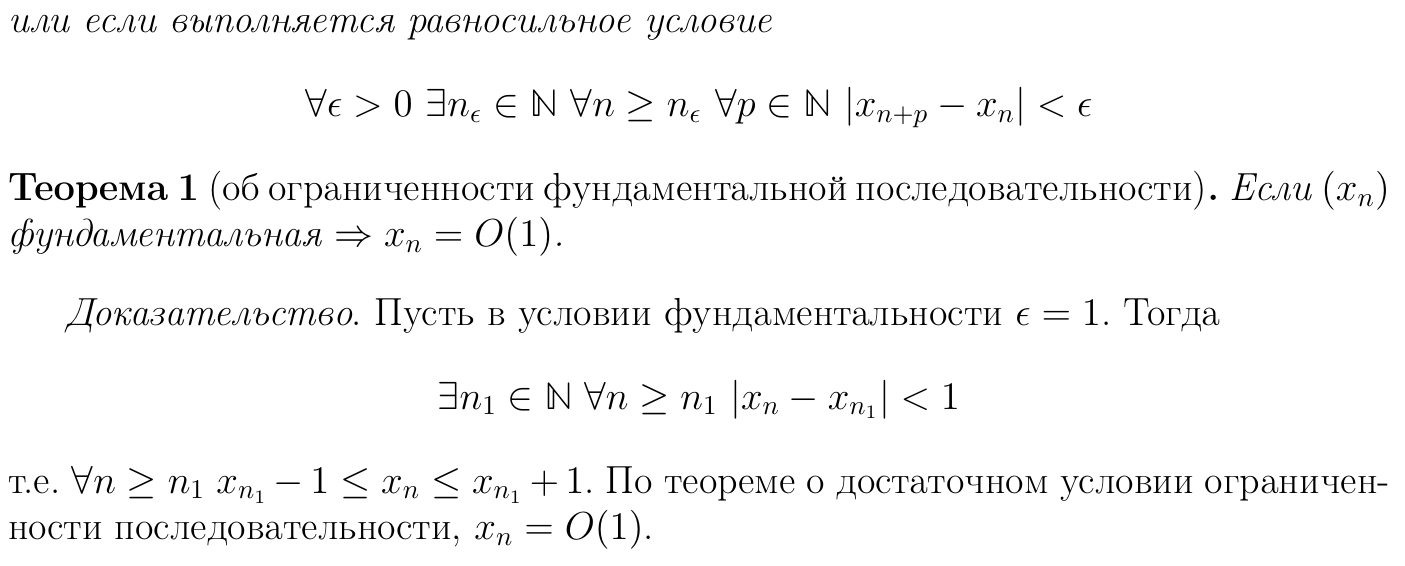
\includegraphics[width=17cm,height=6.847cm]{D0ADD0BAD0B7D0B0D0BCD0B5D0BDD0BED182D0B2D0B5D182D18B-img031.png}
 

\subsection{Критерий Коши сходимости последовательности.}
  [Warning: Image ignored] % Unhandled or unsupported graphics:
%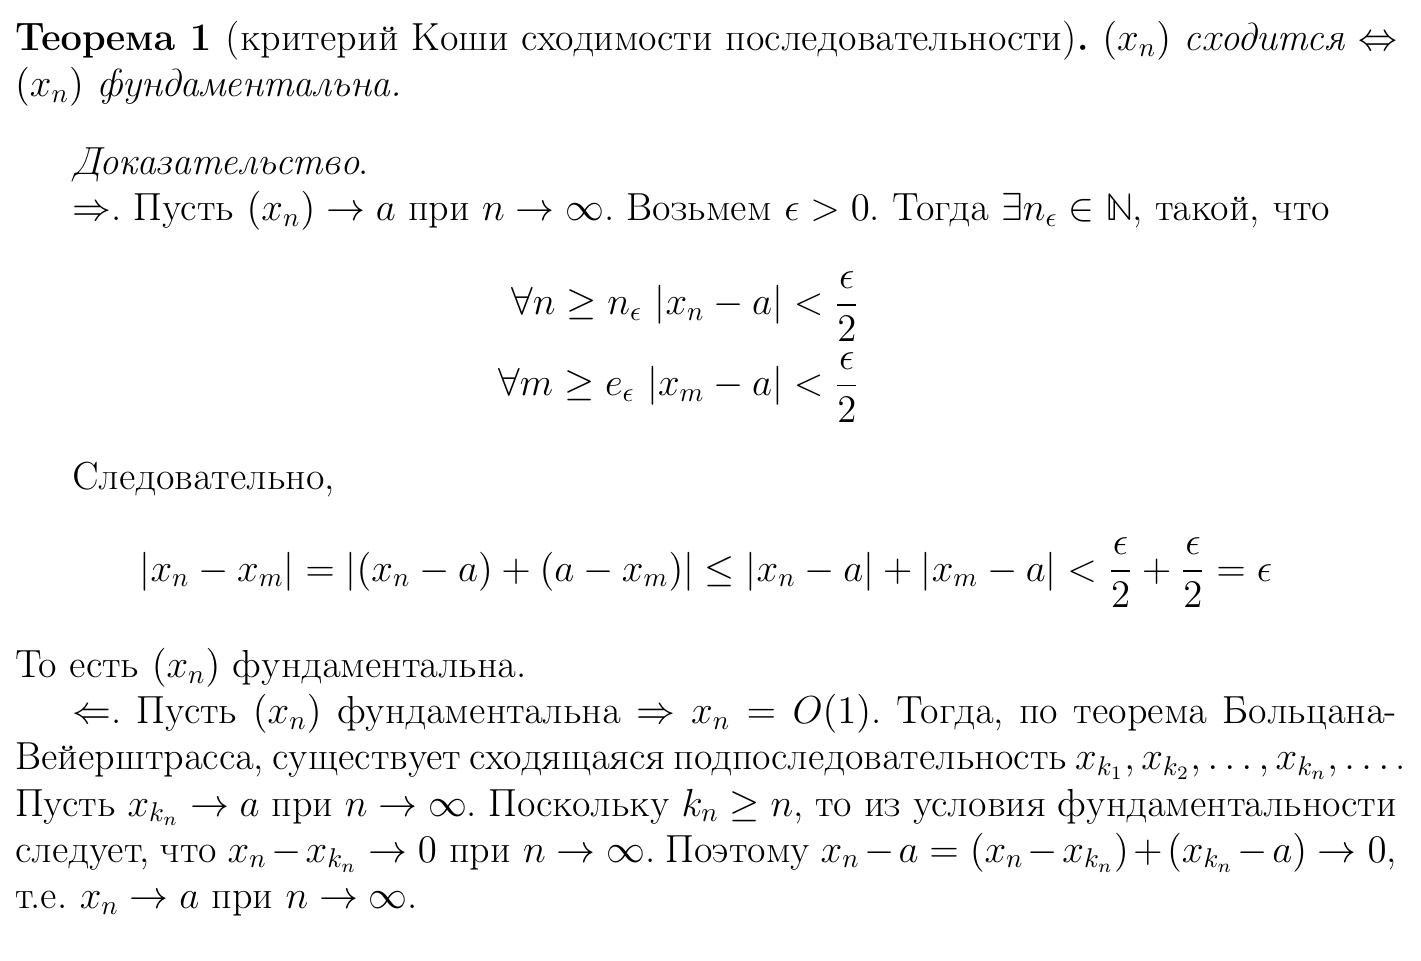
\includegraphics[width=17cm,height=11.497cm]{D0ADD0BAD0B7D0B0D0BCD0B5D0BDD0BED182D0B2D0B5D182D18B-img032.png}
 

\subsection{Определения Гейне и Коши предела функции в точке. Теорема об их эквивалентности.}
  [Warning: Image ignored] % Unhandled or unsupported graphics:
%
\includegraphics[width=17cm,height=1.933cm]{D0ADD0BAD0B7D0B0D0BCD0B5D0BDD0BED182D0B2D0B5D182D18B-img033.png}
 

  [Warning: Image ignored] % Unhandled or unsupported graphics:
%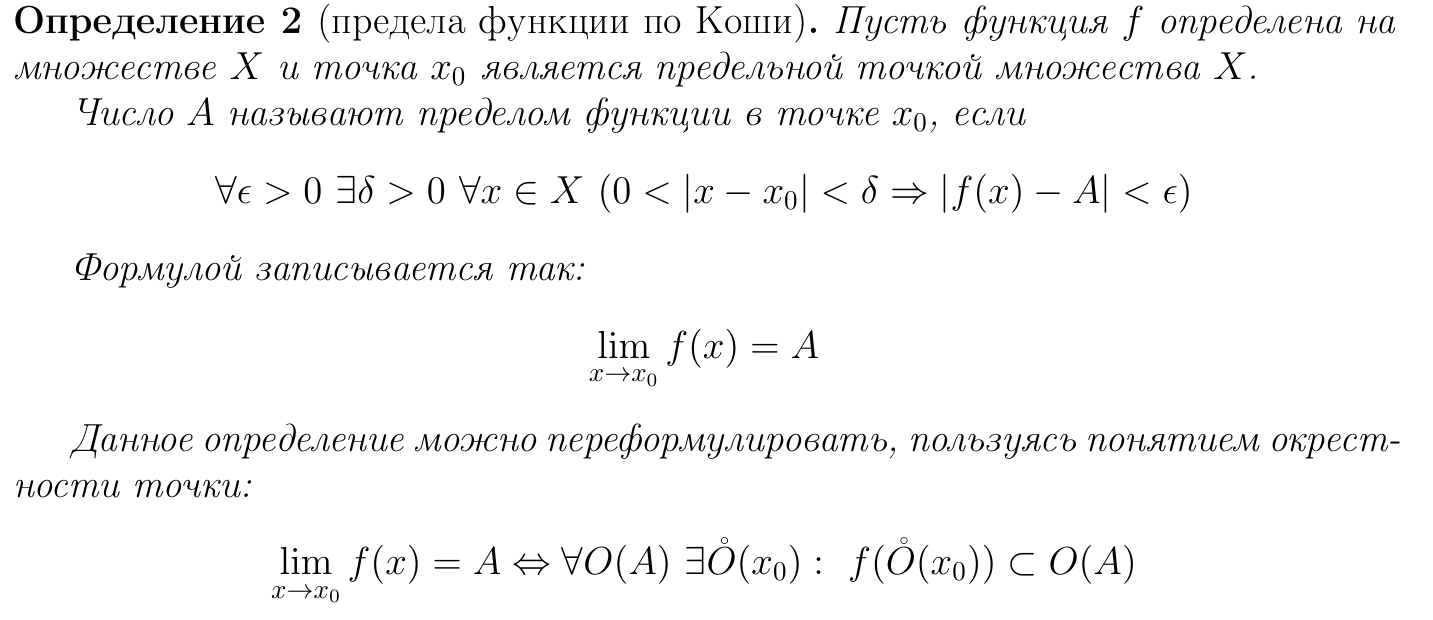
\includegraphics[width=17cm,height=7.355cm]{D0ADD0BAD0B7D0B0D0BCD0B5D0BDD0BED182D0B2D0B5D182D18B-img034.png}
 

  [Warning: Image ignored] % Unhandled or unsupported graphics:
%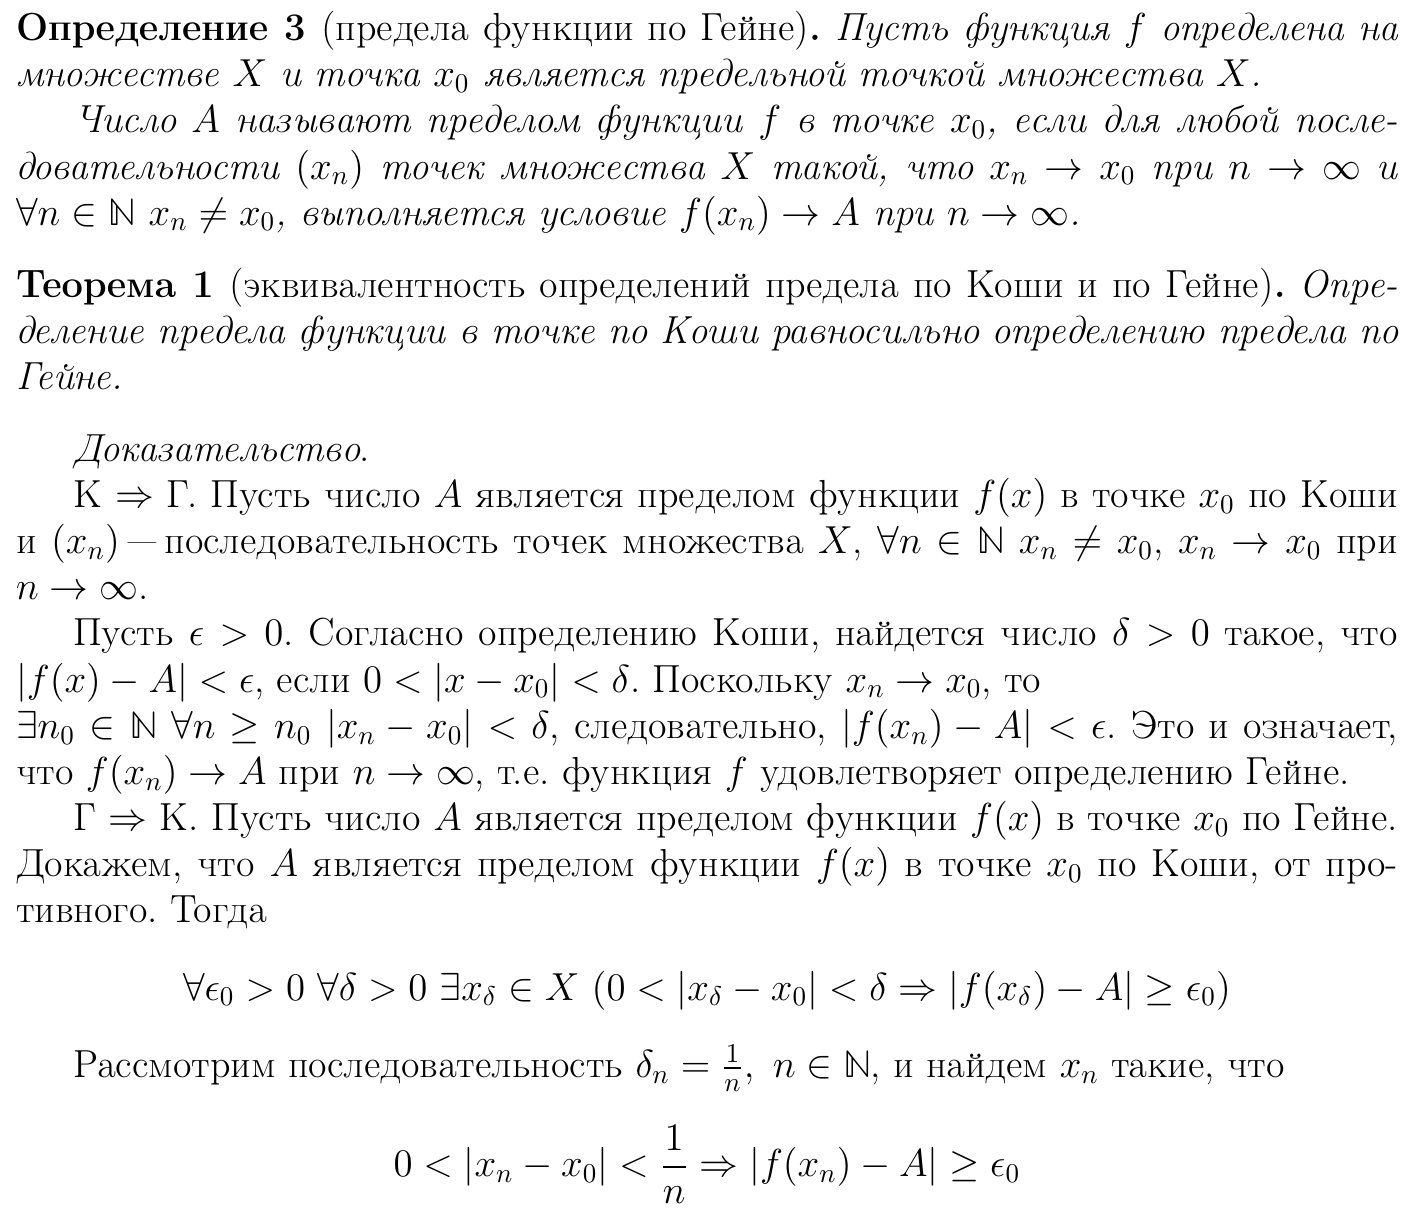
\includegraphics[width=17cm,height=14.501cm]{D0ADD0BAD0B7D0B0D0BCD0B5D0BDD0BED182D0B2D0B5D182D18B-img035.png}
 

  [Warning: Image ignored] % Unhandled or unsupported graphics:
%
\includegraphics[width=17cm,height=2cm]{D0ADD0BAD0B7D0B0D0BCD0B5D0BDD0BED182D0B2D0B5D182D18B-img036.png}
 


\bigskip

\subsection{Критерий Коши существования предела функции.}
  [Warning: Image ignored] % Unhandled or unsupported graphics:
%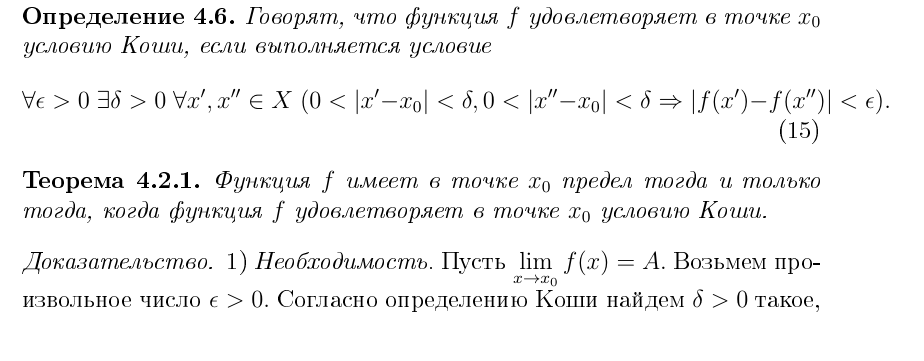
\includegraphics[width=17cm,height=2.327cm]{D0ADD0BAD0B7D0B0D0BCD0B5D0BDD0BED182D0B2D0B5D182D18B-img037.png}
   [Warning: Image ignored] % Unhandled or unsupported graphics:
%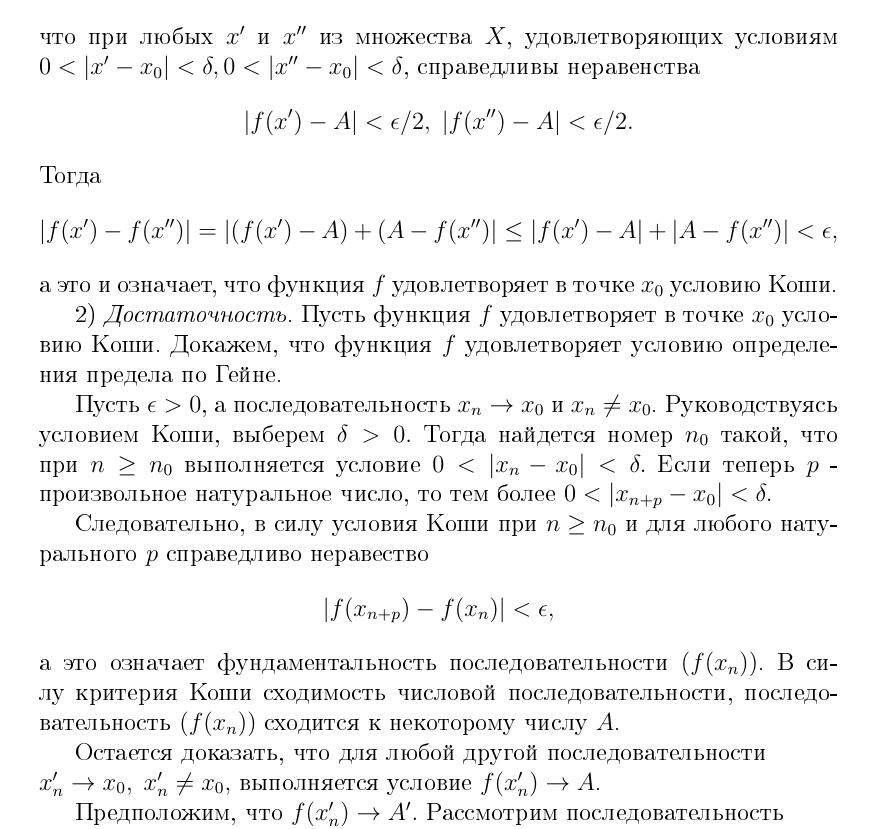
\includegraphics[width=17cm,height=0.45cm]{D0ADD0BAD0B7D0B0D0BCD0B5D0BDD0BED182D0B2D0B5D182D18B-img038.png}
 

\begin{equation*}
\begin{gathered}\boldsubformula{\mathit{\text{К}\text{р}\text{и}\text{т}\text{е}\text{р}\text{и}\text{й}}\mathit{\text{К}\text{о}\text{ш}\text{и}}\mathit{\text{с}\text{у}\text{щ}\text{е}\text{с}\text{т}\text{в}\text{о}\text{в}\text{а}\text{н}\text{и}\text{я}}\mathit{\text{п}\text{р}\text{е}\text{д}\text{е}\text{л}\text{а}}\mathit{\text{ф}\text{у}\text{н}\text{к}\text{ц}\text{и}\text{и}}\text{в}\mathit{\text{т}\text{о}\text{ч}\text{к}\text{е}}(4.2.1).}\\\exists
\lim _{x->x_0}f(x)\Leftrightarrow
f\mathit{\text{у}\text{д}\text{о}\text{в}\text{л}\text{е}\text{т}\text{в}\text{о}\text{р}\text{я}\text{е}\text{т}}\text{в}\mathit{\text{т}.}x_0\mathit{\text{у}\text{с}\text{л}\text{о}\text{в}\text{и}\text{ю}}\mathit{\text{К}\text{о}\text{ш}\text{и}}\\\boldsubformula{\mathit{\text{Д}\text{о}\text{к}\text{а}\text{з}\text{а}\text{т}\text{е}\text{л}\text{ь}\text{с}\text{т}\text{в}\text{о}}}_{\normalsubformula{(\text{в}\mathit{\text{с}\text{о}\text{к}\text{р}\text{а}\text{щ}\text{е}\text{н}\text{и}\text{и}}\mathit{\text{о}\text{т}}\mathit{\text{Д}\text{а}\text{н}\text{и}}):}}\\\Rightarrow
\mathit{\text{П}\text{у}\text{с}\text{т}\text{ь}}\lim _{x->x_0}f(x)=A,\epsilon
>0.\mathit{\text{П}\text{о}}\mathit{\text{о}\text{п}\text{р}\text{е}\text{д}\text{е}\text{л}\text{е}\text{н}\text{и}\text{ю}}\mathit{\text{п}\text{р}\text{е}\text{д}\text{е}\text{л}\text{а}}\mathit{\text{ф}\text{у}\text{н}\text{к}\text{ц}\text{и}\text{и}}\mathit{\text{К}\text{о}\text{ш}\text{и}}\exists
\delta >0\mathit{\text{т}\text{а}\text{к}\text{о}\text{е}},\mathit{\text{ч}\text{т}\text{о}}\\(1)\forall x'\in
X(0<|x'-x_0|<\delta \Rightarrow |f(x')-A|<\mathit{frac}\epsilon 2)\\(2)\forall x''\in X(0<|x''-x_0|<\delta \Rightarrow
|f(x')-A|<\mathit{frac}\epsilon
2)\\\mathit{\text{Т}\text{о}\text{г}\text{д}\text{а}}|f(x')-f(x'')|=|(f(x')-A)+(A-f(x''))|\le
|f(x')-A|+|A-f(x'')|<\frac{\epsilon } 2+\mathit{frac}\epsilon 2=\epsilon \Rightarrow
\\\mathit{\text{ф}\text{у}\text{н}\text{к}\text{ц}\text{и}\text{я}}f\mathit{\text{у}\text{д}\text{о}\text{в}\text{л}\text{е}\text{т}\text{в}\text{о}\text{р}\text{я}\text{е}\text{т}}\text{в}\mathit{\text{т}\text{о}\text{ч}\text{к}\text{е}}x_0\mathit{\text{у}\text{с}\text{л}\text{о}\text{в}\text{и}\text{ю}}\mathit{\text{К}\text{о}\text{ш}\text{и}.}\\{}\\\Leftarrow
\mathit{\text{П}\text{у}\text{с}\text{т}\text{ь}}f\mathit{\text{у}\text{д}\text{о}\text{в}\text{л}\text{е}\text{т}\text{в}\text{о}\text{р}\text{я}\text{е}\text{т}}\text{в}\mathit{\text{т}\text{о}\text{ч}\text{к}\text{е}}x_0\mathit{\text{у}\text{с}\text{л}\text{о}\text{в}\text{и}\text{ю}}\mathit{\text{К}\text{о}\text{ш}\text{и}.}\mathit{\text{Д}\text{о}\text{к}\text{а}\text{ж}\text{е}\text{м}},\mathit{\text{ч}\text{т}\text{о}}f\mathit{\text{у}\text{д}\text{о}\text{в}\text{л}\text{е}\text{т}\text{в}\text{о}\text{р}\text{я}\text{е}\text{т}}\mathit{\text{у}\text{с}\text{л}\text{о}\text{в}\text{и}\text{ю}}\\\mathit{\text{о}\text{п}\text{р}\text{е}\text{д}\text{е}\text{л}\text{е}\text{н}\text{и}\text{я}}\mathit{\text{п}\text{р}\text{е}\text{д}\text{е}\text{л}\text{а}}\mathit{\text{п}\text{о}}\mathit{\text{Г}\text{е}\text{й}\text{н}\text{е}.}\mathit{\text{П}\text{у}\text{с}\text{т}\text{ь}}\epsilon
>0,x_n->x_0\text{и}x_n\neq
x_{0.}\mathit{\text{П}\text{о}}\mathit{\text{у}\text{с}\text{л}\text{о}\text{в}\text{и}\text{ю}}\mathit{\text{К}\text{о}\text{ш}\text{и}}\\\mathit{\text{в}\text{ы}\text{б}\text{е}\text{р}\text{е}\text{м}}\delta
>0\mathit{\text{т}\text{а}\text{к}\text{о}\text{е}},\mathit{\text{ч}\text{т}\text{о}}\\\exists n_0\in \mathbb{N}\forall
n\ge n_0(0<|x_n-x_0|<\delta
).\mathit{\text{Т}\text{е}\text{м}}\mathit{\text{б}\text{о}\text{л}\text{е}\text{е}},\forall p\in
\mathbb{N}0<|x_{n+p}-x_0|<\delta
.\\\text{В}\mathit{\text{с}\text{и}\text{л}\text{у}}\mathit{\text{у}\text{с}\text{л}\text{о}\text{в}\text{и}\text{я}}\mathit{\text{К}\text{о}\text{ш}\text{и}}\forall
n\ge n_0\forall p\in \mathbb{N}|f(x_{n+p})-f(x_n)|<\epsilon \Rightarrow
(f(x_n))-\mathit{\text{ф}\text{у}\text{н}\text{д}.}\\\mathit{\text{п}\text{о}\text{с}\text{л}\text{е}\text{д}\text{о}\text{в}\text{а}\text{т}\text{е}\text{л}\text{ь}\text{н}\text{о}\text{с}\text{т}\text{ь}}\Rightarrow
\text{в}\mathit{\text{с}\text{и}\text{л}\text{у}}\mathit{\text{к}\text{р}\text{и}\text{т}\text{е}\text{р}\text{и}\text{я}}\mathit{\text{К}\text{о}\text{ш}\text{и}}\mathit{\text{с}\text{х}\text{о}\text{д}\text{и}\text{м}\text{о}\text{с}\text{т}\text{и}}\mathit{\text{п}\text{о}\text{с}\text{л}\text{е}\text{д}\text{о}\text{в}\text{а}\text{т}\text{е}\text{л}\text{ь}\text{н}\text{о}\text{с}\text{т}\text{и}}\\(f(x_n))\mathit{\text{с}\text{х}\text{о}\text{д}\text{и}\text{т}\text{с}\text{я}}\text{к}\mathit{\text{н}\text{е}\text{к}\text{о}\text{т}\text{о}\text{р}\text{о}\text{м}\text{у}}\mathit{A.}\\\mathit{\text{Д}\text{о}\text{к}\text{а}\text{ж}\text{е}\text{м}},\mathit{\text{ч}\text{т}\text{о}}\forall
x'_n->x_{0,}x'_n\neq
x_0\mathit{\text{в}\text{ы}\text{п}\text{о}\text{л}\text{н}\text{я}\text{е}\text{т}\text{с}\text{я}}\mathit{\text{у}\text{с}\text{л}\text{о}\text{в}\text{и}\text{е}}f(x'_n)->\mathit{A.}\\\mathit{\text{П}\text{р}\text{е}\text{д}\text{п}\text{о}\text{л}\text{о}\text{ж}\text{и}\text{м}},\mathit{\text{ч}\text{т}\text{о}}f(x'_n)->A'.\mathit{\text{Р}\text{а}\text{с}\text{с}\text{м}\text{о}\text{т}\text{р}\text{и}\text{м}}\mathit{\text{п}\text{о}\text{с}\text{л}\text{е}\text{д}\text{о}\text{в}\text{а}\text{т}\text{е}\text{л}\text{ь}\text{н}\text{о}\text{с}\text{т}\text{ь}}\\x_{1,}x'_{1,}x_{2,}x'_{2,}...,x_n,x'_n,...,\\\mathit{\text{к}\text{о}\text{т}\text{о}\text{р}\text{а}\text{я}}\mathit{\text{т}\text{о}\text{ж}\text{е}}\mathit{\text{с}\text{х}\text{о}\text{д}\text{и}\text{т}\text{с}\text{я}}\text{к}x_{0.}\text{В}\mathit{\text{с}\text{и}\text{л}\text{у}}\mathit{\text{д}\text{о}\text{к}\text{а}\text{з}\text{а}\text{н}\text{н}\text{о}\text{г}\text{о}}\mathit{\text{в}\text{ы}\text{ш}\text{е}},\mathit{\text{п}\text{о}\text{с}\text{л}\text{е}\text{д}\text{о}\text{в}\text{а}\text{т}\text{е}\text{л}\text{ь}\text{н}\text{о}\text{с}\text{т}\text{ь}}\\f(x_1),f(x'_1),f(x_2),f(x'_2),...,f(x_n),f(x'_n),...\\\mathit{\text{с}\text{х}\text{о}\text{д}\text{и}\text{т}\text{с}\text{я}}\text{к}\mathit{\text{н}\text{е}\text{к}\text{о}\text{т}\text{о}\text{р}\text{о}\text{м}\text{у}}\mathit{\text{ч}\text{и}\text{с}\text{л}\text{у}}A''.\mathit{\text{Т}\text{о}\text{г}\text{д}\text{а}}\mathit{\text{е}\text{ё}}\mathit{\text{п}\text{о}\text{д}\text{п}\text{о}\text{с}\text{л}\text{е}\text{д}\text{о}\text{в}\text{а}\text{т}\text{е}\text{л}\text{ь}\text{н}\text{о}\text{с}\text{т}\text{и}}(f(x_n))\text{и}\\(f(x'_n))\mathit{\text{т}\text{о}\text{ж}\text{е}}\mathit{\text{с}\text{х}\text{о}\text{д}\text{я}\text{т}\text{с}\text{я}}\text{к}\mathit{\text{ч}\text{и}\text{с}\text{л}\text{у}}A''\Rightarrow
A=A'=A''\\\mathit{\text{Т}\text{е}\text{о}\text{р}\text{е}\text{м}\text{а}}\mathit{\text{д}\text{о}\text{к}\text{а}\text{з}\text{а}\text{н}\text{а}.}\end{gathered}
\end{equation*}
\subsection{Односторонние пределы функции, связь с пределом.}
Определение левостороннего предела\newline
Определение правостороннего предела

  [Warning: Image ignored] % Unhandled or unsupported graphics:
%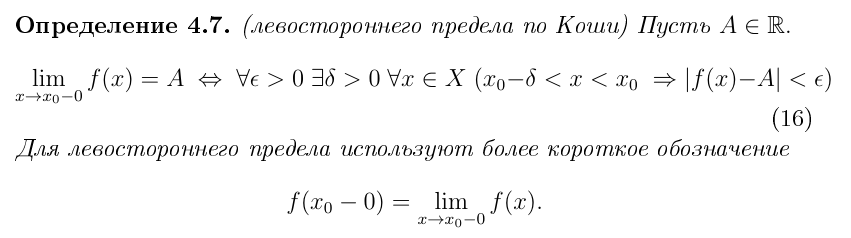
\includegraphics[width=17cm,height=4.754cm]{D0ADD0BAD0B7D0B0D0BCD0B5D0BDD0BED182D0B2D0B5D182D18B-img039.png}
 \newline
  [Warning: Image ignored] % Unhandled or unsupported graphics:
%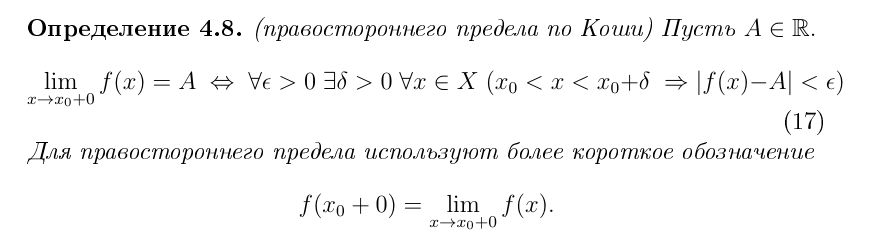
\includegraphics[width=17cm,height=4.674cm]{D0ADD0BAD0B7D0B0D0BCD0B5D0BDD0BED182D0B2D0B5D182D18B-img040.png}
 

Они же на языке окрестностей:

  [Warning: Image ignored] % Unhandled or unsupported graphics:
%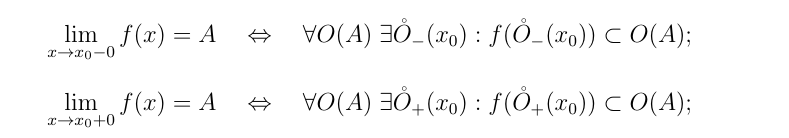
\includegraphics[width=17cm,height=2.972cm]{D0ADD0BAD0B7D0B0D0BCD0B5D0BDD0BED182D0B2D0B5D182D18B-img041.png}
 

\begin{equation*}
\begin{gathered}\boldsubformula{\mathit{\text{Т}\text{е}\text{о}\text{р}\text{е}\text{м}\text{а}}\text{о}\mathit{\text{с}\text{в}\text{я}\text{з}\text{и}}\mathit{\text{о}\text{д}\text{н}\text{о}\text{с}\text{т}\text{о}\text{р}\text{о}\text{н}\text{н}\text{и}\text{х}}\mathit{\text{п}\text{р}\text{е}\text{д}\text{е}\text{л}\text{о}\text{в}}\text{с}\mathit{\text{п}\text{р}\text{е}\text{д}\text{е}\text{л}\text{о}\text{м}}\mathit{\text{ф}\text{у}\text{н}\text{к}\text{ц}\text{и}\text{и}}(4.3.1)}\\\exists
\lim _{x->x_0}f(x)\overset{\mathit{df}}{\Leftrightarrow }\exists \lim _{x->x_0-0}f(x)=\exists \lim
_{x->x_0+0}f(x)=A\\._{\normalsubformula{\mathit{\text{Д}\text{о}\text{к}\text{а}\text{з}\text{а}\text{т}\text{е}\text{л}\text{ь}\text{с}\text{т}\text{в}\text{о}}\mathit{\text{т}\text{р}\text{и}\text{в}\text{и}\text{а}\text{л}\text{ь}\text{н}\text{о}},\mathit{\text{з}\text{н}\text{а}\text{т}\text{ь}}\mathit{\text{т}\text{о}\text{л}\text{ь}\text{к}\text{о}}\mathit{\text{ф}\text{о}\text{р}\text{м}\text{у}\text{л}\text{и}\text{р}\text{о}\text{в}\text{к}\text{у}}}}\end{gathered}
\end{equation*}
\subsection{Арифметические свойства предела функции.}
\begin{equation*}
\begin{gathered}\boldsubformula{\mathit{\text{Т}\text{е}\text{о}\text{р}\text{е}\text{м}\text{а}}\mathit{\text{о}\text{б}}\mathit{\text{а}\text{р}\text{и}\text{ф}\text{м}\text{е}\text{т}\text{и}\text{ч}\text{е}\text{с}\text{к}\text{и}\text{х}}\mathit{\text{с}\text{в}\text{о}\text{й}\text{с}\text{т}\text{в}\text{а}\text{х}}\mathit{\text{п}\text{р}\text{е}\text{д}\text{е}\text{л}\text{а}}\mathit{\text{ф}\text{у}\text{н}\text{к}\text{ц}\text{и}\text{и}}(4.4.1)}\\\mathit{\text{П}\text{у}\text{с}\text{т}\text{ь}}\lim
_{x->x_0}f(x)=A,\lim _{x->x_0}g(x)=\mathit{B.}\mathit{\text{Т}\text{о}\text{г}\text{д}\text{а}}\\\lim _{x->x_0}(f(x)\pm
g(x))=A\pm B,\\\lim _{x->x_0}(f(x)g(x))=\mathit{AB},\\\lim
_{x->x_0}(\mathit{frac}f(x)g(x))=\mathit{frac}AB\normalsubformula{(\mathit{\text{п}\text{р}\text{и}}B\neq
0)}\\{}\\\mathit{\text{Д}\text{о}\text{к}\text{а}\text{з}\text{а}\text{т}\text{е}\text{л}\text{ь}\text{с}\text{т}\text{в}\text{о}}_{(\text{в}\mathit{\text{с}\text{о}\text{к}\text{р}\text{а}\text{щ}\text{е}\text{н}\text{и}\text{и}}\mathit{\text{о}\text{т}}\mathit{\text{Д}\text{а}\text{н}\text{и}})}:\\\mathit{\text{П}\text{у}\text{с}\text{т}\text{ь}}x_n->x_0\text{и}x_n\neq
x_{0.}\mathit{\text{Т}\text{о}\text{г}\text{д}\text{а}}f(x_n)->A\text{и}g(x_n)->\mathit{B.}\\\mathit{\text{П}\text{о}}\mathit{\text{т}\text{е}\text{о}\text{р}\text{е}\text{м}\text{е}}\mathit{\text{о}\text{б}}\mathit{\text{а}\text{р}\text{и}\text{ф}\text{м}\text{е}\text{т}\text{и}\text{ч}\text{е}\text{с}\text{к}\text{и}\text{х}}\mathit{\text{с}\text{в}\text{о}\text{й}\text{с}\text{т}\text{в}\text{а}\text{х}}\mathit{\text{п}\text{р}\text{е}\text{д}\text{е}\text{л}\text{а}}\mathit{\text{п}\text{о}\text{с}\text{л}\text{е}\text{д}\text{о}\text{в}\text{а}\text{т}\text{е}\text{л}\text{ь}\text{н}\text{о}\text{с}\text{т}\text{и}}\mathit{\text{и}\text{м}\text{е}\text{е}\text{м}}:\\f(x_n)\pm
g(x_n)->A\pm B,f(x_n)g(x_n)->\mathit{AB},\frac{f(x_n)}{g(x_n)}->\mathit{frac}AB\Rightarrow
\mathit{\text{п}\text{о}}\mathit{\text{о}\text{п}\text{р}\text{е}\text{д}\text{е}\text{л}\text{е}\text{н}\text{и}\text{ю}}\mathit{\text{Г}\text{е}\text{й}\text{н}\text{е}}:\\\lim
_{x->x_0}(f(x)\pm g(x))=A\pm B,\\\lim _{x->x_0}(f(x)g(x))=\mathit{AB},\\\lim
_{x->x_0}(\mathit{frac}f(x)g(x))=A/B\\\mathit{\text{Т}\text{е}\text{о}\text{р}\text{е}\text{м}\text{а}}\mathit{\text{д}\text{о}\text{к}\text{а}\text{з}\text{а}\text{н}\text{а}.}\end{gathered}
\end{equation*}
\subsection{Порядковые свойства предела функции.}
\begin{equation*}
\begin{gathered}\boldsubformula{\mathit{\text{Т}\text{е}\text{о}\text{р}\text{е}\text{м}\text{а}}\text{о}\mathit{\text{п}\text{о}\text{р}\text{я}\text{д}\text{к}\text{о}\text{в}\text{ы}\text{х}}\mathit{\text{с}\text{в}\text{о}\text{й}\text{с}\text{т}\text{в}\text{а}\text{х}}\mathit{\text{п}\text{р}\text{е}\text{д}\text{е}\text{л}\text{а}}\mathit{\text{ф}\text{у}\text{н}\text{к}\text{ц}\text{и}\text{и}}(4.4.2)}\\\mathit{\text{П}\text{у}\text{с}\text{т}\text{ь}}\lim
_{x->x_0}f(x)=A,\lim _{x->x_0}f(x)=B\text{и}A<\mathit{B.}\mathit{\text{Т}\text{о}\text{г}\text{д}\text{а}}\exists
\multiscripts{}{{}}o{O}{_{\epsilon }}(x_0)\cap
Xf(x)<g(x)\\{}\\\mathit{\text{Д}\text{о}\text{к}\text{а}\text{з}\text{а}\text{т}\text{е}\text{л}\text{ь}\text{с}\text{т}\text{в}\text{о}}:\\\mathit{\text{О}\text{т}}\mathit{\text{п}\text{р}\text{о}\text{т}\text{и}\text{в}\text{н}\text{о}\text{г}\text{о}.}\mathit{\text{П}\text{у}\text{с}\text{т}\text{ь}}\exists
x_n->x_{0,}x_n\neq x_0\mathit{\text{т}\text{а}\text{к}\text{а}\text{я}},\mathit{\text{ч}\text{т}\text{о}}f(x_n)\ge
g(x_n)\Rightarrow \lim _{n->x_0}f(x_n)\lim _{n->x_0}g(x_n)\Rightarrow A\ge B\Rightarrow
\\\mathit{\text{п}\text{р}\text{о}\text{т}\text{и}\text{в}\text{о}\text{р}\text{е}\text{ч}\text{и}\text{е}.}\\\mathit{\text{Т}\text{е}\text{о}\text{р}\text{е}\text{м}\text{а}}\mathit{\text{д}\text{о}\text{к}\text{а}\text{з}\text{а}\text{н}\text{а}.}\\{}\\\mathit{\text{С}\text{л}\text{е}\text{д}\text{с}\text{т}\text{в}\text{и}\text{е}}:\\\mathit{\text{П}\text{у}\text{с}\text{т}\text{ь}}\lim
_{x->x_0}f(x)=A,\lim _{x->x_0}f(x)=B,C\in
\mathit{setR.}\mathit{\text{Т}\text{о}\text{г}\text{д}\text{а}},\mathit{\text{е}\text{с}\text{л}\text{и}}\exists
\multiscripts{}{{}}o{O}{_{\epsilon }}(x_0),\forall x\in \multiscripts{}{{}}o{O}{_{\epsilon
}}(x_0),\\f(x)>g(x)\Rightarrow A\ge B\\f(x)\ge g(x)\Rightarrow A\ge B\\f(x)>C\Rightarrow A\ge C\\f(x)\ge C\Rightarrow
A\ge C\\{}\end{gathered}
\end{equation*}

\bigskip

\subsection{Порядковый признак существования предела функции.}
\begin{equation*}
\begin{gathered}\boldsubformula{\mathit{\text{П}\text{о}\text{р}\text{я}\text{д}\text{к}\text{о}\text{в}\text{ы}\text{й}}\mathit{\text{п}\text{р}\text{и}\text{з}\text{н}\text{а}\text{к}}\mathit{\text{с}\text{у}\text{щ}\text{е}\text{с}\text{т}\text{в}\text{о}\text{в}\text{а}\text{н}\text{и}\text{я}}\mathit{\text{п}\text{р}\text{е}\text{д}\text{е}\text{л}\text{а}}\mathit{\text{ф}\text{у}\text{н}\text{к}\text{ц}\text{и}\text{и}}(4.4.3)}\\\lim
_{x->x_0}f(x)=\lim _{x->x_0}g(x),\forall x\in \multiscripts{}{{}}o{O}{_{\delta }}(x_0)f(x)\le h(x)\le g(x)\Rightarrow
\lim
_{x->x_0}h(x)=\mathit{A.}\\\mathit{\text{Д}\text{о}\text{к}\text{а}\text{з}\text{а}\text{т}\text{е}\text{л}\text{ь}\text{с}\text{т}\text{в}\text{о}}:\\\mathit{\text{П}\text{у}\text{с}\text{т}\text{ь}}x_n->x_0\text{и}x_n\neq
x_{0.}\mathit{\text{Т}\text{о}\text{г}\text{д}\text{а}}f(x_n)\le h(x_n)\le g(x_n)\text{и}\lim _{n->x_0}f(x)=\lim
_{n->x_0}g(x)=A\Rightarrow
\mathit{\text{п}\text{о}}\\\mathit{\text{п}\text{о}\text{р}\text{я}\text{д}\text{к}\text{о}\text{в}\text{о}\text{м}\text{у}}\mathit{\text{п}\text{р}\text{и}\text{з}\text{н}\text{а}\text{к}\text{у}}\mathit{\text{с}\text{у}\text{щ}\text{е}\text{с}\text{т}\text{в}\text{о}\text{в}\text{а}\text{н}\text{и}\text{я}}\mathit{\text{п}\text{р}\text{е}\text{д}\text{е}\text{л}\text{а}}\mathit{\text{п}\text{о}\text{с}\text{л}\text{е}\text{д}\text{о}\text{в}\text{а}\text{т}\text{е}\text{л}\text{ь}\text{н}\text{о}\text{с}\text{т}\text{и}}\exists
\lim _{n->x_0}h(x_n)=A\Rightarrow
\mathit{\text{п}\text{о}}\\\mathit{\text{о}\text{п}\text{р}\text{е}\text{д}\text{е}\text{л}\text{е}\text{н}\text{и}\text{ю}}\mathit{\text{п}\text{р}\text{е}\text{д}\text{е}\text{л}\text{а}}\mathit{\text{Г}\text{е}\text{й}\text{н}\text{е}}\lim
_{x->x_0}h(x)=\mathit{A.}\\\mathit{\text{Т}\text{е}\text{о}\text{р}\text{е}\text{м}\text{а}}\mathit{\text{д}\text{о}\text{к}\text{а}\text{з}\text{а}\text{н}\text{а}.}\end{gathered}
\end{equation*}
\subsection{Теорема о пределе сложной функции.}
\begin{equation*}
\begin{gathered}\boldsubformula{\mathit{\text{Т}\text{е}\text{о}\text{р}\text{е}\text{м}\text{а}}\text{о}\mathit{\text{п}\text{р}\text{е}\text{д}\text{е}\text{л}\text{е}}\mathit{\text{с}\text{л}\text{о}\text{ж}\text{н}\text{о}\text{й}}\mathit{\text{ф}\text{у}\text{н}\text{к}\text{ц}\text{и}\text{и}}(4.4.5)}\\\forall
x\in \overset o{O}(x_0)\lim _{x->x_0}g(x)=y_{0,}g(x)\neq y_0\text{и}\lim _{y->y_0}f(y)=A\Rightarrow \lim
_{x->x_0}f(g(x))=A\\\mathit{\text{Д}\text{о}\text{к}\text{а}\text{з}\text{а}\text{т}\text{е}\text{л}\text{ь}\text{с}\text{т}\text{в}\text{о}}:\\\mathit{\text{В}\text{о}\text{з}\text{ь}\text{м}\text{ё}\text{м}}(x_n)\mathit{\text{и}\text{з}}\overset
o{O}(x_0):x_n->x_{0.}\mathit{\text{Т}\text{о}\text{г}\text{д}\text{а}}y_n=g(x_n)->y_0\text{и}y_n\neq
y_{0,}f(g(x_n))=f(y_n)->A\Rightarrow
\mathit{\text{п}\text{о}}\mathit{\text{о}\text{п}\text{р}\text{е}\text{д}\text{е}\text{л}\text{е}\text{н}\text{и}\text{ю}}\\\mathit{\text{Г}\text{е}\text{й}\text{н}\text{е}}\lim
_{x->x_0}f(g(x))=A\\\mathit{\text{Т}\text{е}\text{о}\text{р}\text{е}\text{м}\text{а}}\mathit{\text{д}\text{о}\text{к}\text{а}\text{з}\text{а}\text{н}\text{а}.}\end{gathered}
\end{equation*}
\subsection{Непрерывность функции в точке. Свойства функций непрерывных в точке.}
\begin{equation*}
\begin{gathered}\boldsubformula{\mathit{\text{О}\text{п}\text{р}\text{е}\text{д}\text{е}\text{л}\text{е}\text{н}\text{и}\text{е}}\mathit{\text{н}\text{е}\text{п}\text{р}\text{е}\text{р}\text{ы}\text{в}\text{н}\text{о}\text{с}\text{т}\text{и}}\mathit{\text{ф}\text{у}\text{н}\text{к}\text{ц}\text{и}\text{и}}\text{в}\mathit{\text{т}\text{о}\text{ч}\text{к}\text{е}}}\\\mathit{\text{П}\text{у}\text{с}\text{т}\text{ь}}f\mathit{\text{о}\text{п}\text{р}\text{е}\text{д}\text{е}\text{л}\text{е}\text{н}\text{а}}\mathit{\text{н}\text{а}}X,x_0\in
X-\mathit{\text{п}\text{р}\text{е}\text{д}\text{е}\text{л}\text{ь}\text{н}\text{а}\text{я}}\mathit{\text{т}\text{о}\text{ч}\text{к}\text{а}}\mathit{x.}\\f\mathit{\text{н}\text{е}\text{п}\text{р}.}\text{в}\mathit{\text{т}.}x_0\overset{\mathit{df}}{\Leftrightarrow
}\mathit{\text{в}\text{ы}\text{п}\text{о}\text{л}\text{н}\text{я}\text{е}\text{т}\text{с}\text{я}}\mathit{\text{х}\text{о}\text{т}\text{я}}\mathit{\text{б}\text{ы}}\mathit{\text{о}\text{д}\text{н}\text{о}}\mathit{\text{и}\text{з}}\mathit{\text{у}\text{с}\text{л}\text{о}\text{в}\text{и}\text{й}}:\\(1)\forall
\epsilon >0\exists \delta >0\forall x\in X(|x-x_0|<\delta \Rightarrow |f(x)-f(x_0)|<\epsilon
)(\mathit{\text{о}\text{п}\text{р}.}\mathit{\text{п}\text{р}\text{е}\text{д}\text{е}\text{л}\text{а}}\mathit{\text{п}\text{о}}\mathit{\text{К}\text{о}\text{ш}\text{и}})\\(2)\forall
O(f(x_0))\exists O(x_0):f(O(x_0))\subset O(f(x_0))\\(3)\forall
(x_n):x_n->x_0f(x_n)->f(x_0)(\mathit{\text{о}\text{п}\text{р}.}\mathit{\text{п}\text{р}\text{е}\text{д}\text{е}\text{л}\text{а}}\mathit{\text{п}\text{о}}\mathit{\text{Г}\text{е}\text{й}\text{н}\text{е}})\\(4)\lim
_{x->x_0}f(x)=f(x_0)\\(5)f(x)=f(x_0)+\alpha (x),\mathit{\text{г}\text{д}\text{е}}\alpha
(x)-\mathit{\text{б}\text{е}\text{с}\text{к}.}\mathit{\text{м}\text{а}\text{л}\text{а}\text{я}}\mathit{\text{п}\text{р}\text{и}}x->x_0\\{}\end{gathered}
\end{equation*}
\begin{equation*}
\begin{gathered}f(x)\mathit{\text{н}\text{е}\text{п}\text{р}.}\mathit{\text{с}\text{л}\text{е}\text{в}\text{а}}\overset{\mathit{df}}{\Leftrightarrow
}\lim
_{x->x_0-0}f(x)=f(x_0)\\f(x)\mathit{\text{н}\text{е}\text{п}\text{р}.}\mathit{\text{с}\text{п}\text{р}\text{а}\text{в}\text{а}}\overset{\mathit{df}}{\Leftrightarrow
}\lim _{x->x_0+0}f(x)=f(x_0)\end{gathered}
\end{equation*}

$\begin{gathered}\boldsubformula{\mathit{\text{Т}\text{е}\text{о}\text{р}\text{е}\text{м}\text{а}}\text{о}\mathit{\text{н}\text{е}\text{п}\text{р}\text{е}\text{р}\text{ы}\text{в}\text{н}\text{о}\text{с}\text{т}\text{и}}\mathit{\text{ф}\text{у}\text{н}\text{к}\text{ц}\text{и}\text{и}}\text{в}\mathit{\text{т}\text{о}\text{ч}\text{к}\text{е}}(5.1.1)}\\f-\mathit{\text{н}\text{е}\text{п}\text{р}}\overset{\mathit{df}}{\Leftrightarrow
}f\mathit{\text{н}\text{е}\text{п}\text{р}.}\mathit{\text{с}\text{п}\text{р}\text{а}\text{в}\text{а}}\wedge
f\mathit{\text{н}\text{е}\text{п}\text{р}.}\mathit{\text{с}\text{л}\text{е}\text{в}\text{а}}\end{gathered}$\newline

$\begin{gathered}\boldsubformula{\mathit{\text{Т}\text{е}\text{о}\text{р}\text{е}\text{м}\text{а}}\text{о}\mathit{\text{с}\text{в}\text{о}\text{й}\text{с}\text{т}\text{в}\text{а}\text{х}}\mathit{\text{н}\text{е}\text{п}\text{р}\text{е}\text{р}\text{ы}\text{в}\text{н}\text{ы}\text{х}}\mathit{\text{ф}\text{у}\text{н}\text{к}\text{ц}\text{и}\text{й}}(5.1.2)}\\\mathit{\text{П}\text{у}\text{с}\text{т}\text{ь}}f\text{и}g-\mathit{\text{н}\text{е}\text{п}\text{р}.}\text{в}\mathit{\text{т}.}x_0.\mathit{\text{Т}\text{о}\text{г}\text{д}\text{а}}\\(1)\forall
a,b\in
\mathbb{R}\mathit{af}+\mathit{bg}-\mathit{\text{н}\text{е}\text{п}\text{р}.}\text{в}\mathit{\text{т}.}x_0\\(2)\mathit{fg}-\mathit{\text{н}\text{е}\text{п}\text{р}.}\text{в}\mathit{\text{т}.}x_0(3)f/g-\mathit{\text{н}\text{е}\text{п}\text{р}}\text{в}\mathit{\text{т}.}x_0(\mathit{\text{п}\text{р}\text{и}}g(x_0)\neq
0)\\(4)f(x_0)\neq 0\Rightarrow \exists O(x_0)\forall x\in
O(x_0)f(x)f(x_0)>0(\mathit{\text{т}.}\mathit{\text{е}.}f(x)\mathit{\text{с}\text{о}\text{х}\text{р}\text{а}\text{н}\text{я}\text{е}\text{т}}\mathit{\text{з}\text{н}\text{а}\text{к}})\\(5)f\mathit{\text{л}\text{о}\text{к}\text{а}\text{л}\text{ь}\text{н}\text{о}}\mathit{\text{о}\text{г}\text{р}\text{а}\text{н}\text{и}\text{ч}\text{е}\text{н}\text{а}}\text{в}O(x_0)\end{gathered}$

\begin{figure}
\centering
 [Warning: Image ignored] % Unhandled or unsupported graphics:
%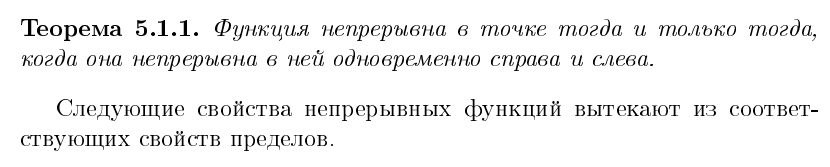
\includegraphics[width=17cm,height=0.346cm]{D0ADD0BAD0B7D0B0D0BCD0B5D0BDD0BED182D0B2D0B5D182D18B-img042.png}

\end{figure}
\subsection{Непрерывность функции на множестве. Теорема об обращении функции в нуль и теорема Коши о промежуточных
значениях функции.}
\begin{equation*}
\begin{gathered}f-\mathit{\text{н}\text{е}\text{п}\text{р}.}\mathit{\text{н}\text{а}}X\overset{\mathit{df}}{\Leftrightarrow
}\forall x\in
Xf-\mathit{\text{н}\text{е}\text{п}\text{р}.}\text{в}x\\f-\mathit{\text{н}\text{е}\text{п}\text{р}.}\overset{\mathit{df}}{\Leftrightarrow
}\forall x\in D(f)f-\mathit{\text{н}\text{е}\text{п}\text{р}.}\text{в}x\end{gathered}
\end{equation*}
Теорема Коши об обращении функции в нуль

  [Warning: Image ignored] % Unhandled or unsupported graphics:
%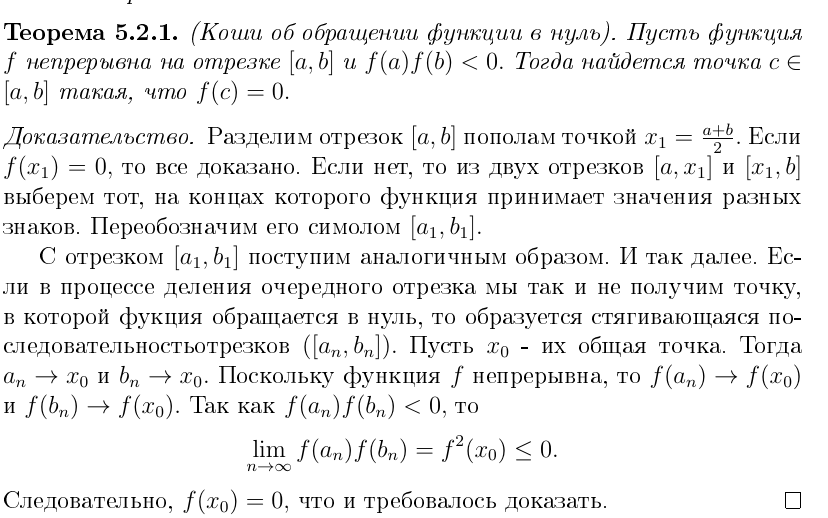
\includegraphics[width=17cm,height=9.932cm]{D0ADD0BAD0B7D0B0D0BCD0B5D0BDD0BED182D0B2D0B5D182D18B-img043.png}
 

\begin{equation*}
\begin{gathered}\boldsubformula{\mathit{\text{Т}\text{е}\text{о}\text{р}\text{е}\text{м}\text{а}}\mathit{\text{К}\text{о}\text{ш}\text{и}}\text{о}\mathit{\text{п}\text{р}\text{о}\text{м}\text{е}\text{ж}\text{у}\text{т}\text{о}\text{ч}\text{н}\text{ы}\text{х}}\mathit{\text{з}\text{н}\text{а}\text{ч}\text{е}\text{н}\text{и}\text{я}\text{х}}\mathit{\text{ф}\text{у}\text{н}\text{к}\text{ц}\text{и}\text{и}}(5.2.2.)}\\f-\mathit{\text{н}\text{е}\text{п}\text{р}.}\mathit{\text{н}\text{а}}[a,b],f(a)=A,f(b)=B,A\neq
B,C-\mathit{\text{л}\text{ю}\text{б}\text{о}\text{е}}\mathit{\text{ч}\text{и}\text{с}\text{л}\text{о}}\mathit{\text{м}\text{е}\text{ж}\text{д}\text{у}}A\text{и}B\Rightarrow
\exists c\in
[a,b]f(c)=C\\\mathit{\text{Д}\text{о}\text{к}\text{а}\text{з}\text{а}\text{т}\text{е}\text{л}\text{ь}\text{с}\text{т}\text{в}\text{о}}:\\\mathit{\text{Р}\text{а}\text{с}\text{с}\text{м}\text{о}\text{т}\text{р}\text{и}\text{м}}g(x)=f(x)-\mathit{C.}\mathit{\text{П}\text{о}}\mathit{\text{т}\text{е}\text{о}\text{р}\text{е}\text{м}\text{е}}\mathit{\text{К}\text{о}\text{ш}\text{и}}\mathit{\text{о}\text{б}}\mathit{\text{о}\text{б}\text{р}\text{а}\text{щ}\text{е}\text{н}\text{и}\text{и}}\mathit{\text{ф}\text{у}\text{н}\text{к}\text{ц}\text{и}\text{и}}\text{в}\mathit{\text{н}\text{у}\text{л}\text{ь}}\exists
c\in
[a,b]f(c)=\mathit{C.}\\\mathit{\text{Т}\text{е}\text{о}\text{р}\text{е}\text{м}\text{а}}\mathit{\text{д}\text{о}\text{к}\text{а}\text{з}\text{а}\text{н}\text{а}.}\end{gathered}
\end{equation*}
\subsection{Компакт. Теорема об ограниченности компакта. Критерий компактности. }
Определение компактного множества

\begin{equation*}
X\subset
\mathbb{R}-\mathit{\text{к}\text{о}\text{м}\text{п}\text{а}\text{к}\text{т}}\overset{\mathit{df}}{\Leftrightarrow
}\forall (x_n)\exists (y_n)=(x_{k_n}):y_n->x_{0,}x_0\in X
\end{equation*}
\begin{equation*}
\begin{gathered}\mathit{\text{Э}\text{т}\text{и}}3\mathit{\text{о}\text{п}\text{р}\text{е}\text{д}\text{е}\text{л}\text{е}\text{н}\text{и}\text{я}}\mathit{\text{н}\text{е}}\mathit{\text{т}\text{р}\text{е}\text{б}\text{у}\text{ю}\text{т}\text{с}\text{я}}\mathit{\text{д}\text{л}\text{я}}\mathit{\text{о}\text{т}\text{в}\text{е}\text{т}\text{а}}\mathit{\text{н}\text{а}}\mathit{\text{в}\text{о}\text{п}\text{р}\text{о}\text{с}},\mathit{\text{н}\text{о}}\mathit{\text{и}\text{х}}\mathit{\text{з}\text{н}\text{а}\text{н}\text{и}\text{е}}\mathit{\text{н}\text{а}\text{м}}\mathit{\text{о}\text{ч}\text{е}\text{н}\text{ь}}\mathit{\text{п}\text{о}\text{н}\text{а}\text{д}\text{о}\text{б}\text{и}\text{т}\text{с}\text{я}}\mathit{\text{п}\text{о}\text{з}\text{ж}\text{е}}:\\X-\mathit{\text{з}\text{а}\text{м}\text{к}\text{н}\text{у}\text{т}\text{о}\text{е}}\overset{\mathit{df}}{\Leftrightarrow
}X\mathit{\text{с}\text{о}\text{д}\text{е}\text{р}\text{ж}\text{и}\text{т}}\mathit{\text{в}\text{с}\text{е}}\mathit{\text{с}\text{в}\text{о}\text{и}}\mathit{\text{п}\text{р}\text{е}\text{д}\text{е}\text{л}\text{ь}\text{н}\text{ы}\text{е}}\mathit{\text{т}\text{о}\text{ч}\text{к}\text{и}}\\x\in
X-\mathit{\text{в}\text{н}\text{у}\text{т}\text{р}\text{е}\text{н}\text{н}\text{я}\text{я}}\mathit{\text{т}\text{о}\text{ч}\text{к}\text{а}}X\overset{\mathit{df}}{\Leftrightarrow
}\exists O(x)\subset
X\\X-\mathit{\text{о}\text{т}\text{к}\text{р}\text{ы}\text{т}\text{о}\text{е}}\overset{\mathit{df}}{\Leftrightarrow
}\forall x\in Xx-\mathit{\text{в}\text{н}\text{у}\text{т}\text{р}.}\end{gathered}
\end{equation*}
Теорема об ограниченности компакта

  [Warning: Image ignored] % Unhandled or unsupported graphics:
%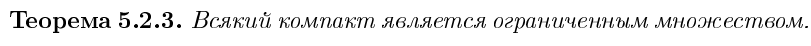
\includegraphics[width=17cm,height=0.961cm]{D0ADD0BAD0B7D0B0D0BCD0B5D0BDD0BED182D0B2D0B5D182D18B-img044.png}
 

  [Warning: Image ignored] % Unhandled or unsupported graphics:
%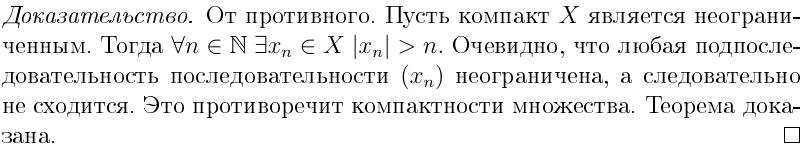
\includegraphics[width=17cm,height=3.297cm]{D0ADD0BAD0B7D0B0D0BCD0B5D0BDD0BED182D0B2D0B5D182D18B-img045.png}
 

\begin{equation*}
\begin{gathered}\boldsubformula{\mathit{\text{К}\text{р}\text{и}\text{т}\text{е}\text{р}\text{и}\text{й}}\mathit{\text{к}\text{о}\text{м}\text{п}\text{а}\text{к}\text{т}\text{н}\text{о}\text{с}\text{т}\text{и}}(5.2.4.)}\\X-\mathit{\text{к}\text{о}\text{м}\text{п}\text{а}\text{к}\text{т}}\overset{\mathit{df}}{\Leftrightarrow
}X-\mathit{\text{о}\text{г}\text{р}.}\wedge
X\mathit{\text{з}\text{а}\text{м}\text{к}\text{н}\text{у}\text{т}\text{о}}\\\mathit{\text{Д}\text{о}\text{к}\text{а}\text{з}\text{а}\text{т}\text{е}\text{л}\text{ь}\text{с}\text{т}\text{в}\text{о}}:\\\Rightarrow
\mathit{\text{П}\text{у}\text{с}\text{т}\text{ь}}X-\mathit{\text{к}\text{о}\text{м}\text{п}\text{а}\text{к}\text{т}.}\mathit{\text{П}\text{о}}\mathit{\text{т}\text{е}\text{о}\text{р}\text{е}\text{м}\text{е}}\mathit{\text{о}\text{б}}\mathit{\text{о}\text{г}\text{р}\text{а}\text{н}\text{и}\text{ч}\text{е}\text{н}\text{н}\text{о}\text{с}\text{т}\text{и}}\mathit{\text{к}\text{о}\text{м}\text{п}\text{а}\text{к}\text{т}\text{а}}x-\mathit{\text{о}\text{г}\text{р}.}\mathit{\text{Д}\text{о}\text{к}\text{а}\text{ж}\text{е}\text{м}}\mathit{\text{з}\text{а}\text{м}\text{к}\text{н}\text{у}\text{т}\text{о}\text{с}\text{т}\text{ь}.}\\\mathit{\text{П}\text{у}\text{с}\text{т}\text{ь}}x_0-\mathit{\text{п}\text{р}\text{е}\text{д}\text{е}\text{л}\text{ь}\text{н}\text{а}\text{я}}\mathit{\text{т}\text{о}\text{ч}\text{к}\text{а}}\mathit{X.}\mathit{\text{Т}\text{о}\text{г}\text{д}\text{а}}\exists
(x_n):x_n->x_{0,}x_n\neq
x_{0.}\mathit{\text{П}\text{о}}\mathit{\text{о}\text{п}\text{р}\text{е}\text{д}\text{е}\text{л}\text{е}\text{н}\text{и}\text{ю}}\mathit{\text{к}\text{о}\text{м}\text{п}\text{а}\text{к}\text{т}\text{н}\text{о}\text{с}\text{т}\text{и}}\\\exists
(x_{n_k}):x_{n_k}->x'_0\in
\mathit{X.}\text{В}\mathit{\text{т}\text{о}}\mathit{\text{ж}\text{е}}\mathit{\text{в}\text{р}\text{е}\text{м}\text{я}}x_n->x_0\Rightarrow
x_{n_k}->x_{0.}\mathit{\text{С}\text{л}\text{е}\text{д}\text{о}\text{в}\text{а}\text{т}\text{е}\text{л}\text{ь}\text{н}\text{о}},x_0=x'_0\in
\mathit{X.}\\{}\\\Leftarrow
\mathit{\text{П}\text{у}\text{с}\text{т}\text{ь}}X-\mathit{\text{о}\text{г}\text{р}.}\text{и}\mathit{\text{з}\text{а}\text{м}\text{к}\text{н}\text{у}\text{т}\text{о}.}\mathit{\text{В}\text{о}\text{з}\text{ь}\text{м}\text{ё}\text{м}}(x_n).\forall
n\in \mathbb{N}x_n\in X\Rightarrow (x_n)-\mathit{\text{о}\text{г}\text{р}.}\Rightarrow
\mathit{\text{п}\text{о}}\mathit{\text{т}\text{е}\text{о}\text{р}\text{е}\text{м}\text{е}}\\\mathit{\text{Б}\text{о}\text{л}\text{ь}\text{ц}\text{а}\text{н}\text{о}}-\mathit{\text{В}\text{е}\text{й}\text{е}\text{р}\text{ш}\text{т}\text{р}\text{а}\text{с}\text{с}\text{а}}\exists
(x_{n_k})\end{gathered}
\end{equation*}
\subsection{Теорема о непрерывном образе компакта. Первая и вторая теоремы Вейерштрасса.}
Теорема о непрерывном образе компакта

  [Warning: Image ignored] % Unhandled or unsupported graphics:
%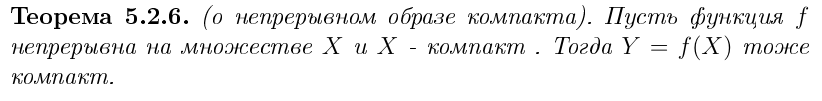
\includegraphics[width=17cm,height=2.087cm]{D0ADD0BAD0B7D0B0D0BCD0B5D0BDD0BED182D0B2D0B5D182D18B-img046.png}
 

  [Warning: Image ignored] % Unhandled or unsupported graphics:
%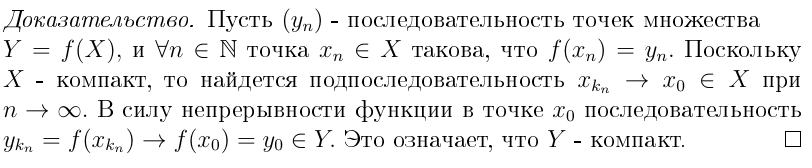
\includegraphics[width=17cm,height=3.515cm]{D0ADD0BAD0B7D0B0D0BCD0B5D0BDD0BED182D0B2D0B5D182D18B-img047.png}
 

\begin{equation*}
\begin{gathered}\boldsubformula{\mathit{\text{Т}\text{е}\text{о}\text{р}\text{е}\text{м}\text{а}}\text{о}\mathit{\text{н}\text{е}\text{п}\text{р}\text{е}\text{р}\text{ы}\text{в}\text{н}\text{о}\text{м}}\mathit{\text{о}\text{б}\text{р}\text{а}\text{з}\text{е}}\mathit{\text{к}\text{о}\text{м}\text{п}\text{а}\text{к}\text{т}\text{а}}(5.2.6.)}\\f\mathit{\text{н}\text{е}\text{п}\text{р}.}\mathit{\text{н}\text{а}}X,X-\mathit{\text{к}\text{о}\text{м}\text{п}\text{а}\text{к}\text{т}}\Rightarrow
Y=f(X)-\mathit{\text{к}\text{о}\text{м}\text{п}\text{а}\text{к}\text{т}}\\\mathit{\text{Д}\text{о}\text{к}\text{а}\text{з}\text{а}\text{т}\text{е}\text{л}\text{ь}\text{с}\text{т}\text{в}\text{о}}:\\\mathit{\text{П}\text{у}\text{с}\text{т}\text{ь}}(y_n)-\mathit{\text{п}\text{о}\text{с}\text{л}\text{е}\text{д}\text{о}\text{в}\text{а}\text{т}\text{е}\text{л}\text{ь}\text{н}\text{о}\text{с}\text{т}\text{ь}}\mathit{\text{т}\text{о}\text{ч}\text{е}\text{к}}\mathit{\text{м}\text{н}\text{о}\text{ж}\text{е}\text{с}\text{т}\text{в}\text{а}}Y=f(X),\forall
n\in \mathbb{N}x_n\in Xf(x_n)=y_n.\\X-\mathit{\text{к}\text{о}\text{м}\text{п}\text{а}\text{к}\text{т}}\Rightarrow
\exists x_{k_n}->x_0\in
\mathit{X.}\text{В}\mathit{\text{с}\text{и}\text{л}\text{у}}\mathit{\text{н}\text{е}\text{п}\text{р}\text{е}\text{р}\text{ы}\text{в}\text{н}\text{о}\text{с}\text{т}\text{и}}f\text{в}\mathit{\text{т}.}x_0y_{k_n}=f(x_{k_n})->f(x_0)=y_o\in
Y\Rightarrow
Y-\mathit{\text{к}\text{о}\text{м}\text{п}\text{а}\text{к}\text{т}.}\\\mathit{\text{Т}\text{е}\text{о}\text{р}\text{е}\text{м}\text{а}}\mathit{\text{д}\text{о}\text{к}\text{а}\text{з}\text{а}\text{н}\text{а}.}\end{gathered}
\end{equation*}
Первая теорема Вейерштрасса\newline
Вторая теорема Вейерштрасса

  [Warning: Image ignored] % Unhandled or unsupported graphics:
%
\includegraphics[width=17cm,height=3.224cm]{D0ADD0BAD0B7D0B0D0BCD0B5D0BDD0BED182D0B2D0B5D182D18B-img048.png}
 

\subsection{Равномерная непрерывность функции и теорема Кантора.}
Определение равномерно непрерывной функции

  [Warning: Image ignored] % Unhandled or unsupported graphics:
%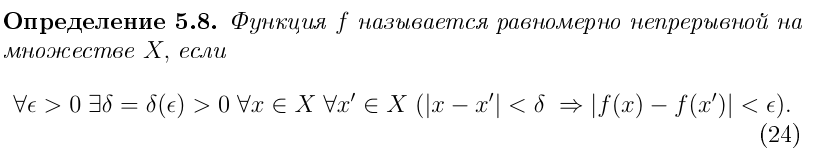
\includegraphics[width=17cm,height=3.482cm]{D0ADD0BAD0B7D0B0D0BCD0B5D0BDD0BED182D0B2D0B5D182D18B-img049.png}
 

\begin{equation*}
\begin{gathered}\boldsubformula{\mathit{\text{Т}\text{е}\text{о}\text{р}\text{е}\text{м}\text{а}}\mathit{\text{К}\text{а}\text{н}\text{т}\text{о}\text{р}\text{а}}(5.3.1.)}\\f-\mathit{\text{н}\text{е}\text{п}\text{р}.}\mathit{\text{н}\text{а}}\mathit{\text{к}\text{о}\text{м}\text{п}\text{а}\text{к}\text{т}\text{е}}X\Rightarrow
f\mathit{\text{р}\text{а}\text{в}\text{н}\text{о}\text{м}\text{е}\text{р}\text{н}\text{о}}\mathit{\text{н}\text{е}\text{п}\text{р}\text{е}\text{р}\text{ы}\text{в}\text{н}\text{а}}\mathit{\text{н}\text{а}}X\\\mathit{\text{Д}\text{о}\text{к}\text{а}\text{з}\text{а}\text{т}\text{е}\text{л}\text{ь}\text{с}\text{т}\text{в}\text{о}}:\\\mathit{\text{О}\text{т}}\mathit{\text{п}\text{р}\text{о}\text{т}\text{и}\text{в}\text{н}\text{о}\text{г}\text{о}.}\mathit{\text{П}\text{у}\text{с}\text{т}\text{ь}}f\mathit{\text{н}\text{е}\text{п}\text{р}.}\mathit{\text{н}\text{а}}X\text{и}\neg
(\mathit{\text{р}\text{а}\text{в}\text{н}\text{о}\text{м}\text{е}\text{р}\text{н}\text{о}}\mathit{\text{н}\text{е}\text{п}\text{р}\text{е}\text{р}\text{ы}\text{в}\text{н}\text{а}}\mathit{\text{н}\text{а}}X).\mathit{\text{Т}\text{о}\text{г}\text{д}\text{а}}\\\exists
\epsilon _0>0\forall \delta >0\exists x',x''\in X(|x'-x''|<\delta \Rightarrow |f(x')-f(x'')|\ge \epsilon
_0)\\\mathit{\text{П}\text{у}\text{с}\text{т}\text{ь}}\delta _n=\frac
1{\mathit{n.}}\mathit{\text{Т}\text{о}\text{г}\text{д}\text{а}}\forall n\in \mathbb{N}\exists
x'_n,x''_n|x'_n-x''_n|<\frac 1 n,\mathit{\text{н}\text{о}}|f(x'_n)-f(x''_n)|\ge \epsilon
_0\\X-\mathit{\text{к}\text{о}\text{м}\text{п}\text{а}\text{к}\text{т}}->\exists x'_{k_n}->x_0\in X\text{и}\exists
x''_{k_n}->x_0\in \mathit{X.}\\f-\mathit{\text{н}\text{е}\text{п}\text{р}.}\Rightarrow f(x'_{k_n})->f(x_0)\in
X\text{и}f(x''_{k_n})=f(x_0)\Rightarrow f(x'_{k_n})-f(x''_{k_n})->0\Rightarrow
\mathit{\text{п}\text{р}\text{о}\text{т}\text{и}\text{в}\text{о}\text{р}\text{е}\text{ч}\text{и}\text{е}}\\\mathit{\text{Т}\text{е}\text{о}\text{р}\text{е}\text{м}\text{а}}\mathit{\text{д}\text{о}\text{к}\text{а}\text{з}\text{а}\text{н}\text{а}.}\end{gathered}
\end{equation*}
\subsection{Односторонние пределы. Точки разрыва функции и их классификация. Теорема об односторонних пределах
монотонной функции.}
\begin{equation*}
\begin{gathered}\mathit{\text{П}\text{у}\text{с}\text{т}\text{ь}}f\mathit{\text{о}\text{п}\text{р}\text{е}\text{д}\text{е}\text{л}\text{е}\text{н}\text{а}}\text{в}\overset
o{O}(x_0).\\x_0-\mathit{\text{т}.}\mathit{\text{у}\text{с}\text{т}\text{р}\text{а}\text{н}\text{и}\text{м}\text{о}\text{г}\text{о}}\mathit{\text{р}\text{а}\text{з}\text{р}\text{ы}\text{в}\text{а}}\overset{\mathit{df}}{\Leftrightarrow
}\exists \lim
_{x->x_0}f(x),\mathit{\text{н}\text{о}}(f\mathit{\text{н}\text{е}}\mathit{\text{о}\text{п}\text{р}.}\text{в}\mathit{\text{т}.}x_0\vee
\lim _{x->x_0}f(x)\neq
f(x_0))\\x_0-\mathit{\text{т}.}\mathit{\text{р}\text{а}\text{з}\text{р}\text{ы}\text{в}\text{а}}\mathit{\text{п}\text{е}\text{р}\text{в}\text{о}\text{г}\text{о}}\mathit{\text{р}\text{о}\text{д}\text{а}}\overset{\mathit{df}}{\Leftrightarrow
}\exists f(x_0-0),f(x_0+0),\mathit{\text{н}\text{о}}f(x_0-0)\neq f(x_0+0),\Delta
f(x_0)=f(x_0-0)-f(x_0+0)\\\mathit{\text{н}\text{а}\text{з}\text{ы}\text{в}\text{а}\text{ю}\text{т}}\mathit{\text{с}\text{к}\text{а}\text{ч}\text{к}\text{о}\text{м}}\mathit{\text{ф}\text{у}\text{н}\text{к}\text{ц}\text{и}\text{и}}\\x_0-\mathit{\text{т}.}\mathit{\text{р}\text{а}\text{з}\text{р}\text{ы}\text{в}\text{а}}\mathit{\text{в}\text{т}\text{о}\text{р}\text{о}\text{г}\text{о}}\mathit{\text{р}\text{о}\text{д}\text{а}}\overset{\mathit{df}}{\Leftrightarrow
}\mathit{\text{х}\text{о}\text{т}\text{я}}\mathit{\text{б}\text{ы}}\mathit{\text{о}\text{д}\text{и}\text{н}}\mathit{\text{и}\text{з}}\mathit{\text{о}\text{д}\text{н}\text{о}\text{с}\text{т}\text{о}\text{р}\text{о}\text{н}\text{н}\text{и}\text{х}}\mathit{\text{п}\text{р}\text{е}\text{д}\text{е}\text{л}\text{о}\text{в}}\mathit{\text{н}\text{е}}\mathit{\text{с}\text{у}\text{щ}}-\text{т}\mathit{\text{и}\text{л}\text{и}}\mathit{\text{р}\text{а}\text{в}\text{е}\text{н}}\mathit{infinity.}\end{gathered}
\end{equation*}
\begin{equation*}
\begin{gathered}\boldsubformula{\mathit{\text{Т}\text{е}\text{о}\text{р}\text{е}\text{м}\text{а}}\mathit{\text{о}\text{б}}\mathit{\text{о}\text{д}\text{н}\text{о}\text{с}\text{т}\text{о}\text{р}\text{о}\text{н}\text{н}\text{и}\text{х}}\mathit{\text{п}\text{р}\text{е}\text{д}\text{е}\text{л}\text{а}\text{х}}\mathit{\text{м}\text{о}\text{н}\text{о}\text{т}\text{о}\text{н}\text{н}\text{о}\text{й}}\mathit{\text{ф}\text{у}\text{н}\text{к}\text{ц}\text{и}\text{и}}(5.4.1.)}\\\mathit{\text{П}\text{у}\text{с}\text{т}\text{ь}}f-\mathit{\text{м}\text{о}\text{н}\text{о}\text{т}\text{о}\text{н}\text{н}\text{а}\text{я}}\mathit{\text{н}\text{а}}(a,b).\mathit{\text{Т}\text{о}\text{г}\text{д}\text{а}}\forall
x_0\in (a,b)\exists
f(x_0-0),f(x_0+0).\mathit{\text{Б}\text{о}\text{л}\text{е}\text{е}}\mathit{\text{т}\text{о}\text{г}\text{о}},\\\mathit{\text{е}\text{с}\text{л}\text{и}}f\uparrow
:\\f(x_0-0)=\underset{x<x_0}{\mathit{su\text{р}}}f(x),f(x_0+0)=\underset{x>x_0}{\mathit{inf}}f(x),\\f(x_0-0)\le
f(x_0)\le f(x_0+0)\\\mathit{\text{е}\text{с}\text{л}\text{и}}f\downarrow
:\\f(x_0-0)=\underset{x<x_0}{\mathit{inf}}f(x),f(x_0+0)=\underset{x>x_0}{\mathit{su\text{р}}}f(x),\\f(x_0-0)\ge
f(x_0)\ge
f(x_0+0)\\\mathit{\text{Д}\text{о}\text{к}\text{а}\text{з}\text{а}\text{т}\text{е}\text{л}\text{ь}\text{с}\text{т}\text{в}\text{о}}:\\\mathit{\text{Р}\text{а}\text{с}\text{с}\text{м}\text{о}\text{т}\text{р}\text{и}\text{м}}\mathit{\text{с}\text{л}\text{у}\text{ч}\text{а}\text{й}}f\mathit{uparrow.}\mathit{\text{Д}\text{о}\text{к}\text{а}\text{ж}\text{е}\text{м}},\mathit{\text{ч}\text{т}\text{о}}f(x_0-0)=\underset{x<x_0}{\mathit{su\text{р}}}f(x).\{f(x):x<x_0\}\mathit{\text{о}\text{г}\text{р}.}\mathit{\text{с}\text{в}\text{е}\text{р}\text{х}\text{у}}\Rightarrow
\\\exists \underset{x<x_0}{\mathit{su\text{р}}}f(x)=l,l\le f(x_0)\Rightarrow
\mathit{\text{п}\text{о}}\mathit{\text{о}\text{п}\text{р}.}\mathit{\text{в}\text{е}\text{р}\text{х}\text{н}\text{е}\text{й}}\mathit{\text{г}\text{р}\text{а}\text{н}\text{и}}:\\1\left.\right)\forall
x<x_0f(x)\le l;\\2\left.\right)\forall \epsilon >0\exists x_{\epsilon }<x_0f(x_{\epsilon })>l-\epsilon \\f\uparrow
\Rightarrow \forall x\in \left[x_{\epsilon
},x_0\right)\mathit{\text{в}\text{ы}\text{п}\text{о}\text{л}\text{н}\text{я}\text{ю}\text{т}\text{с}\text{я}}\mathit{\text{н}\text{е}\text{р}\text{а}\text{в}\text{е}\text{н}\text{с}\text{т}\text{в}\text{а}}l-\epsilon
<f(x_{\epsilon })\le f(x)\le l<l+\epsilon \Rightarrow \\\Rightarrow \lim
_{x->x_0-0}f(x)=l\\\mathit{\text{О}\text{с}\text{т}\text{а}\text{л}\text{ь}\text{н}\text{о}\text{е}}\mathit{\text{д}\text{о}\text{к}\text{а}\text{з}\text{ы}\text{в}\text{а}\text{е}\text{т}\text{с}\text{я}}\mathit{\text{а}\text{н}\text{а}\text{л}\text{о}\text{г}\text{и}\text{ч}\text{н}\text{о}.}\end{gathered}
\end{equation*}
\subsection{Критерий непрерывности монотонной функции. Теорема о непрерывности обратной функции.}
Критерий непрерывности монотонной функции

  [Warning: Image ignored] % Unhandled or unsupported graphics:
%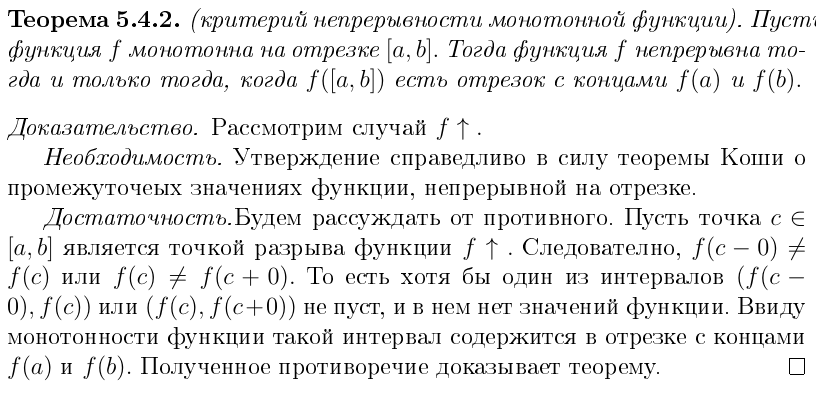
\includegraphics[width=17cm,height=8.207cm]{D0ADD0BAD0B7D0B0D0BCD0B5D0BDD0BED182D0B2D0B5D182D18B-img050.png}
 


\bigskip

Теорема о непрерывности обратной функции

  [Warning: Image ignored] % Unhandled or unsupported graphics:
%\includegraphics[width=17cm,height=6.853cm]{D0ADD0BAD0B7D0B0D0BCD0B5D0BDD0BED182D0B2D0B5D182D18B-img051.png}
 

\subsection{Дифференцируемость функции в точке, производная функции в точке. Непрерывность дифференцируемой функции. }
\begin{equation*}
\begin{gathered}\mathit{\text{П}\text{у}\text{с}\text{т}\text{ь}}f\mathit{\text{о}\text{п}\text{р}.}\mathit{\text{н}\text{а}}X,x_0\in
X-\mathit{\text{п}\text{р}\text{е}\text{д}\text{е}\text{л}\text{ь}\text{н}\text{а}\text{я}}\mathit{\text{т}\text{о}\text{ч}\text{к}\text{а}.}\\f-\mathit{\text{д}\text{и}\text{ф}\text{ф}\text{е}\text{р}\text{е}\text{н}\text{ц}\text{и}\text{р}\text{у}\text{е}\text{м}\text{а}}\text{в}\mathit{\text{т}\text{о}\text{ч}\text{к}\text{е}}x_0\overset{\mathit{df}}{\Leftrightarrow
}\exists
A(x)\mathit{\text{н}\text{е}\text{п}\text{р}\text{е}\text{р}\text{ы}\text{в}\text{н}\text{а}\text{я}}\text{в}\mathit{\text{т}\text{о}\text{ч}\text{к}\text{е}}x_{0,}\forall
x\in
Xf(x)-f(x_0)=A(x)(x-x_0)\\f'(x_0)=A(x_0)-\mathit{\text{п}\text{р}\text{о}\text{и}\text{з}\text{в}\text{о}\text{д}\text{н}\text{а}\text{я}}f\text{в}\mathit{\text{т}.}x_0\end{gathered}
\end{equation*}
\begin{equation*}
\begin{gathered}\boldsubformula{\mathit{\text{Т}\text{е}\text{о}\text{р}\text{е}\text{м}\text{а}}\text{о}\mathit{\text{н}\text{е}\text{п}\text{р}\text{е}\text{р}\text{ы}\text{в}\text{н}\text{о}\text{с}\text{т}\text{и}}\mathit{\text{д}\text{и}\text{ф}\text{ф}\text{е}\text{р}\text{е}\text{н}\text{ц}\text{и}\text{р}\text{у}\text{е}\text{м}\text{о}\text{й}}\mathit{\text{ф}\text{у}\text{н}\text{к}\text{ц}\text{и}\text{и}}(6.1.2.)}\\f-\mathit{\text{д}\text{и}\text{ф}\text{ф}.}\text{в}\mathit{\text{т}.}x_0\Rightarrow
f-\mathit{\text{н}\text{е}\text{п}\text{р}.}\text{в}\mathit{\text{т}.}x_0\\\mathit{\text{Д}\text{о}\text{к}\text{а}\text{з}\text{а}\text{т}\text{е}\text{л}\text{ь}\text{с}\text{т}\text{в}\text{о}}:\\f(x)-f(x_0)=A(x)(x-x_0)\Leftrightarrow
f(x)=f(x_0)+A(x)(x-x_0)\\\mathit{\text{П}\text{о}}\mathit{\text{т}\text{е}\text{о}\text{р}\text{е}\text{м}\text{е}}\text{о}\mathit{\text{с}\text{в}\text{о}\text{й}\text{с}\text{т}\text{в}\text{а}\text{х}}\mathit{\text{н}\text{е}\text{п}\text{р}.}\mathit{\text{ф}\text{у}\text{н}\text{к}\text{ц}\text{и}\text{й}}f(x)\mathit{\text{н}\text{е}\text{п}\text{р}.}\text{в}\mathit{\text{т}.}x_0\\\mathit{\text{Т}\text{е}\text{о}\text{р}\text{е}\text{м}\text{а}}\mathit{\text{д}\text{о}\text{к}\text{а}\text{з}\text{а}\text{н}\text{а}.}\end{gathered}
\end{equation*}
\subsection{Теорема о дифференцируемости композиции.}
  [Warning: Image ignored] % Unhandled or unsupported graphics:
%\includegraphics[width=17cm,height=5.99cm]{D0ADD0BAD0B7D0B0D0BCD0B5D0BDD0BED182D0B2D0B5D182D18B-img052.png}
 

  [Warning: Image ignored] % Unhandled or unsupported graphics:
%\includegraphics[width=17cm,height=15.425cm]{D0ADD0BAD0B7D0B0D0BCD0B5D0BDD0BED182D0B2D0B5D182D18B-img053.png}
 

\subsection{Теорема об арифметических действиях над дифференцируемыми функциями.}
  [Warning: Image ignored] % Unhandled or unsupported graphics:
%\includegraphics[width=17cm,height=23.375cm]{D0ADD0BAD0B7D0B0D0BCD0B5D0BDD0BED182D0B2D0B5D182D18B-img054.png}
 

  [Warning: Image ignored] % Unhandled or unsupported graphics:
%\includegraphics[width=17cm,height=12.474cm]{D0ADD0BAD0B7D0B0D0BCD0B5D0BDD0BED182D0B2D0B5D182D18B-img055.png}
 

\subsection{Теорема о дифференцируемости обратной функции.}
  [Warning: Image ignored] % Unhandled or unsupported graphics:
%\includegraphics[width=17cm,height=11.218cm]{D0ADD0BAD0B7D0B0D0BCD0B5D0BDD0BED182D0B2D0B5D182D18B-img056.png}
 

  [Warning: Image ignored] % Unhandled or unsupported graphics:
%\includegraphics[width=17cm,height=5.299cm]{D0ADD0BAD0B7D0B0D0BCD0B5D0BDD0BED182D0B2D0B5D182D18B-img057.png}
 

\subsection{Точки роста и убывания функции. \ Достаточное условие точек роста и точек убывания.}
Определение точки роста функции\newline
Определение точки убывания функции

  [Warning: Image ignored] % Unhandled or unsupported graphics:
%\includegraphics[width=17cm,height=4.445cm]{D0ADD0BAD0B7D0B0D0BCD0B5D0BDD0BED182D0B2D0B5D182D18B-img058.png}
 

\begin{equation*}
\begin{gathered}\boldsubformula{\mathit{\text{Д}\text{о}\text{с}\text{т}\text{а}\text{т}\text{о}\text{ч}\text{н}\text{о}\text{е}}\mathit{\text{у}\text{с}\text{л}\text{о}\text{в}\text{и}\text{е}}\mathit{\text{т}\text{о}\text{ч}\text{е}\text{к}}\mathit{\text{р}\text{о}\text{с}\text{т}\text{а}}\text{и}\mathit{\text{т}\text{о}\text{ч}\text{е}\text{к}}\mathit{\text{у}\text{б}\text{ы}\text{в}\text{а}\text{н}\text{и}\text{я}}(6.4.1.)}\\f'(x_0)>0(f'(x_0)<0)\Rightarrow
x_0-\mathit{\text{т}\text{о}\text{ч}\text{к}\text{а}}\mathit{\text{р}\text{о}\text{с}\text{т}\text{а}}(\mathit{\text{у}\text{б}\text{ы}\text{в}\text{а}\text{н}\text{и}\text{я}})f\\\mathit{\text{Д}\text{о}\text{к}\text{а}\text{з}\text{а}\text{т}\text{е}\text{л}\text{ь}\text{с}\text{т}\text{в}\text{о}}:\\\mathit{\text{П}\text{о}}\mathit{\text{о}\text{п}\text{р}\text{е}\text{д}\text{е}\text{л}\text{е}\text{н}\text{и}\text{ю}}\mathit{\text{д}\text{и}\text{ф}\text{ф}\text{е}\text{р}\text{е}\text{н}\text{ц}\text{и}\text{р}\text{у}\text{е}\text{м}\text{о}\text{с}\text{т}\text{и}}\mathit{\text{ф}\text{у}\text{н}\text{к}\text{ц}\text{и}\text{и}}\\f(x)-f(x_o)=A(x)(x-x_0),\mathit{\text{г}\text{д}\text{е}}A(x)\mathit{\text{н}\text{е}\text{п}\text{р}.}\text{в}\mathit{\text{т}.}x_{0,}A(x_0)=f'(x_0)\\1\left.\right)f'(x_0)>0\Rightarrow
A(x_0)>0\Rightarrow \exists O(x_0)\forall x\in O(x_0)A(x)>0\Rightarrow \forall x\in
O(x_0)\\\mathit{sign}(f(x)-f(x_0))=\mathit{sign}(A(x)(x-x_0))=\mathit{sign}(x-x_0)\Leftrightarrow
x_0-\mathit{\text{т}.}\mathit{\text{р}\text{о}\text{с}\text{т}\text{а}}\\2\left.\right)f'(x_0)<0\Rightarrow
A(x_0)<0\Rightarrow \exists O(x_0)\forall x\in O(x_0)A(x)<0\Rightarrow \forall x\in
O(x_0)\\\mathit{sign}(f(x)-f(x_0))=\mathit{sign}(A(x)(x-x_0))=-\mathit{sign}(x-x_0)\Leftrightarrow
x_0-\mathit{\text{т}.}\mathit{\text{у}\text{б}\text{ы}\text{в}\text{а}\text{н}\text{и}\text{я}}\end{gathered}
\end{equation*}
\subsection{Точки локального экстремума. Теорема Ферма. }
\begin{equation*}
\begin{gathered}\mathit{\text{П}\text{у}\text{с}\text{т}\text{ь}}x_0-\mathit{\text{в}\text{н}\text{у}\text{т}\text{р}.}\mathit{\text{т}\text{о}\text{ч}\text{к}\text{а}}D(f).\\x_0-\mathit{\text{т}.}\mathit{\text{л}\text{о}\text{к}\text{а}\text{л}\text{ь}\text{н}\text{о}\text{г}\text{о}}\mathit{\text{э}\text{к}\text{с}\text{т}\text{р}\text{е}\text{м}\text{у}\text{м}\text{а}}f\overset{\mathit{df}}{\Leftrightarrow
}\exists O(x_0)\forall x\in O(x_0)f(x)\le f(x_0)(f(x)\ge
f(x_0))\\x_0-\mathit{\text{т}.}\mathit{\text{с}\text{т}\text{р}\text{о}\text{г}\text{о}\text{г}\text{о}}\mathit{\text{л}\text{о}\text{к}\text{а}\text{л}\text{ь}\text{н}\text{о}\text{г}\text{о}}\mathit{\text{э}\text{к}\text{с}\text{т}\text{р}\text{е}\text{м}\text{у}\text{м}\text{а}}\overset{\mathit{df}}{\Leftrightarrow
}\exists \overset o{O}(x_0)\forall x\in \overset o{O}(x_0)f(x)<f(x_0)(f(x)>f(x_0))\end{gathered}
\end{equation*}
\begin{equation*}
\begin{gathered}\boldsubformula{\mathit{\text{Т}\text{е}\text{о}\text{р}\text{е}\text{м}\text{а}}\mathit{\text{Ф}\text{е}\text{р}\text{м}\text{а}}(\mathit{\text{н}\text{е}\text{о}\text{б}\text{х}\text{о}\text{д}\text{и}\text{м}\text{о}\text{е}}\mathit{\text{у}\text{с}\text{л}\text{о}\text{в}\text{и}\text{е}}\mathit{\text{л}\text{о}\text{к}\text{а}\text{л}\text{ь}\text{н}\text{о}\text{г}\text{о}}\mathit{\text{э}\text{к}\text{с}\text{т}\text{р}\text{е}\text{м}\text{у}\text{м}\text{а}},6.4.2.)}\\x_0-\mathit{\text{т}.}\mathit{\text{л}\text{о}\text{к}\text{а}\text{л}\text{ь}\text{н}\text{о}\text{г}\text{о}}\mathit{\text{э}\text{к}\text{с}\text{т}\text{р}\text{е}\text{м}\text{у}\text{м}\text{а}}f\text{и}\exists
f'(x_0)\Rightarrow
f'(x_0)=0\\\mathit{\text{Д}\text{о}\text{к}\text{а}\text{з}\text{а}\text{т}\text{е}\text{л}\text{ь}\text{с}\text{т}\text{в}\text{о}}:\\x_0\mathit{\text{н}\text{е}}\mathit{\text{м}\text{о}\text{ж}\text{е}\text{т}}\mathit{\text{б}\text{ы}\text{т}\text{ь}}\mathit{\text{т}\text{о}\text{ч}\text{к}\text{о}\text{й}}\mathit{\text{р}\text{о}\text{с}\text{т}\text{а}}\mathit{\text{и}\text{л}\text{и}}\mathit{\text{т}\text{о}\text{ч}\text{к}\text{о}\text{й}}\mathit{\text{у}\text{б}\text{ы}\text{в}\text{а}\text{н}\text{и}\text{я}}\Leftrightarrow
f'(x_0)\le 0\wedge f'(x_0)\ge 0\Leftrightarrow
f'(x_0)=0\\\mathit{\text{Т}\text{е}\text{о}\text{р}\text{е}\text{м}\text{а}}\mathit{\text{д}\text{о}\text{к}\text{а}\text{з}\text{а}\text{н}\text{а}}\end{gathered}
\end{equation*}

\bigskip

\subsection{Теорема Ролля.}
  [Warning: Image ignored] % Unhandled or unsupported graphics:
%\includegraphics[width=17cm,height=6.974cm]{D0ADD0BAD0B7D0B0D0BCD0B5D0BDD0BED182D0B2D0B5D182D18B-img059.png}
 

\subsection{Теоремы Коши и Лагранжа. Следствия теоремы Лагранжа.}
Теорема Коши\newline
Теорема Лагранжа

  [Warning: Image ignored] % Unhandled or unsupported graphics:
%\includegraphics[width=17cm,height=6.782cm]{D0ADD0BAD0B7D0B0D0BCD0B5D0BDD0BED182D0B2D0B5D182D18B-img060.png}
 

  [Warning: Image ignored] % Unhandled or unsupported graphics:
%\includegraphics[width=17cm,height=8.632cm]{D0ADD0BAD0B7D0B0D0BCD0B5D0BDD0BED182D0B2D0B5D182D18B-img061.png}
 

Теорема о постоянстве дифференцируемой функции

  [Warning: Image ignored] % Unhandled or unsupported graphics:
%\includegraphics[width=17cm,height=6.849cm]{D0ADD0BAD0B7D0B0D0BCD0B5D0BDD0BED182D0B2D0B5D182D18B-img062.png}
 

Критерий монотонности дифференцируемой функции

  [Warning: Image ignored] % Unhandled or unsupported graphics:
%\includegraphics[width=17cm,height=2.618cm]{D0ADD0BAD0B7D0B0D0BCD0B5D0BDD0BED182D0B2D0B5D182D18B-img063.png}
 

  [Warning: Image ignored] % Unhandled or unsupported graphics:
%\includegraphics[width=17cm,height=8.832cm]{D0ADD0BAD0B7D0B0D0BCD0B5D0BDD0BED182D0B2D0B5D182D18B-img064.png}
 

Достаточное условие строгой монотонности функции

  [Warning: Image ignored] % Unhandled or unsupported graphics:
%\includegraphics[width=17cm,height=3.103cm]{D0ADD0BAD0B7D0B0D0BCD0B5D0BDD0BED182D0B2D0B5D182D18B-img065.png}
 

\subsection{Производные высших порядков. Формула Тейлора. Остаточный член формулы Тейлора \ в форме Лагранжа. }
\begin{equation*}
\begin{gathered}\boldsubformula{\mathit{\text{Ф}\text{о}\text{р}\text{м}\text{у}\text{л}\text{а}}\mathit{\text{Т}\text{е}\text{й}\text{л}\text{о}\text{р}\text{а}}(6.7.1.)}\\fn-\mathit{\text{н}\text{е}\text{п}\text{р}.}\mathit{\text{д}\text{и}\text{ф}\text{ф}.}\mathit{\text{н}\text{а}}\mathit{\text{о}\text{т}\text{р}\text{е}\text{з}\text{к}\text{е}}I\text{с}\mathit{\text{к}\text{о}\text{н}\text{ц}\text{а}\text{м}\text{и}}x_{0,}x\text{и}\exists
f^{(n+1)}\mathit{\text{в}\text{н}\text{у}\text{т}\text{р}\text{и}}\mathit{\text{н}\text{е}\text{г}\text{о}}\Rightarrow
\forall \phi (x):\mathit{\text{н}\text{е}\text{п}\text{р}.}\mathit{\text{н}\text{а}}I\wedge \exists \phi '(x)\neq
0\\\exists \xi
\mathit{\text{в}\text{н}\text{у}\text{т}\text{р}\text{и}}I\mathit{\text{т}\text{а}\text{к}\text{а}\text{я}},\mathit{\text{ч}\text{т}\text{о}}\\f(x)=f(x_0)+\mathit{frac}f'(x_0)1!(x-x_0)+...+\mathit{frac}f^{(n)}(x_0)n!(x-x_0)^n+r_n(x_0;x),\mathit{\text{г}\text{д}\text{е}}\\r_n(x_0;x)=\mathit{frac}\phi
(x)-\phi (x_0)\phi '(\xi )n!f^{(n+1)}(\xi )(x-\xi
)^n\\\mathit{\text{Д}\text{о}\text{к}\text{а}\text{з}\text{а}\text{т}\text{е}\text{л}\text{ь}\text{с}\text{т}\text{в}\text{о}}:\\\mathit{\text{Н}\text{а}}\mathit{\text{о}\text{т}\text{р}.}I\mathit{\text{р}\text{а}\text{с}\text{с}\text{м}\text{о}\text{т}\text{р}\text{и}\text{м}}\mathit{\text{в}\text{с}\text{п}\text{о}\text{м}\text{о}\text{г}\text{а}\text{т}\text{е}\text{л}\text{ь}\text{н}\text{у}\text{ю}}\mathit{\text{ф}\text{у}\text{н}\text{к}\text{ц}\text{и}\text{ю}}\\F(t)=f(x)-P_n(t;x)=f(x)-[f(t)+\mathit{frac}f'(t)1!(x-t)+...+\mathit{frac}f_{(n)}(t)n!(x-t)^n]\\\mathit{\text{О}\text{ч}\text{е}\text{в}\text{и}\text{д}\text{н}\text{о}},\mathit{\text{ч}\text{т}\text{о}}F\mathit{\text{н}\text{е}\text{п}\text{р}\text{е}\text{р}\text{ы}\text{в}\text{н}\text{а}}\mathit{\text{н}\text{а}}\mathit{\text{о}\text{т}\text{р}\text{е}\text{з}\text{к}\text{е}}I\text{и}\mathit{\text{д}\text{и}\text{ф}\text{ф}.}\mathit{\text{в}\text{н}\text{у}\text{т}\text{р}\text{и}}I,\mathit{\text{п}\text{р}\text{и}\text{ч}\text{ё}\text{м}}\\F'(t)=\mathit{frac}-f^{(n+1)}(t)n!(x-t)^n.\\\mathit{\text{П}\text{р}\text{и}\text{м}\text{е}\text{н}\text{я}\text{я}}\text{к}\mathit{\text{п}\text{а}\text{р}\text{е}}\mathit{\text{ф}\text{у}\text{н}\text{к}\text{ц}\text{и}\text{й}}F,\phi
\mathit{\text{н}\text{а}}\mathit{\text{о}\text{т}\text{р}.}I\mathit{\text{т}\text{е}\text{о}\text{р}\text{е}\text{м}\text{у}}\mathit{\text{К}\text{о}\text{ш}\text{и}},\exists
\xi
\mathit{\text{в}\text{н}\text{у}\text{т}\text{р}\text{и}}I,\text{в}\mathit{\text{к}\text{о}\text{т}\text{о}\text{р}\text{о}\text{й}}\mathit{\text{в}\text{ы}\text{п}\text{о}\text{л}\text{н}\text{я}\text{е}\text{т}\text{с}\text{я}}\\\mathit{frac}F(x)-F(x_0)\phi
(x)-\phi (x_0)=\mathit{frac}F'(\xi )\phi '(\xi
).\\\mathit{\text{П}\text{о}\text{с}\text{к}\text{о}\text{л}\text{ь}\text{к}\text{у}}F(x)-F(x_0)=0-F(x_0)=-r_n(x_0;x)\text{и}\\F'(\xi
)=\mathit{frac}-f^{(n+1)}(\xi )n!(x-\xi
)^n,\\\mathit{\text{т}\text{о}}\mathit{\text{п}\text{р}\text{и}\text{х}\text{о}\text{д}\text{и}\text{м}}\text{к}\mathit{\text{р}\text{а}\text{в}\text{е}\text{н}\text{с}\text{т}\text{в}\text{у}}\\r_n(x_0;x)=\mathit{frac}\phi
(x)-\phi (x_0)\phi '(\xi )n!f^{(n+1)}(\xi )(x-\xi )^{\mathit{n.}}\end{gathered}
\end{equation*}

\bigskip

Остаточный член формулы Тейлора в форме Лагранжа

  [Warning: Image ignored] % Unhandled or unsupported graphics:
%\includegraphics[width=17cm,height=3.261cm]{D0ADD0BAD0B7D0B0D0BCD0B5D0BDD0BED182D0B2D0B5D182D18B-img066.png}
 

\subsection[Формула Тейлора{}-Пеано.]{Формула Тейлора-Пеано.}

\bigskip


\bigskip

\begin{equation*}
\begin{gathered}\boldsubformula{\mathit{\text{Л}\text{е}\text{м}\text{м}\text{а}.}}\\\phi \phantom
.n-\mathit{\text{д}\text{и}\text{ф}\text{ф}.}\phantom .\text{в}\phantom .\mathit{\text{т}.}\phantom .x_0\phantom
.\text{и}\phantom .\phi (x_0)=\phi '(x_0)=...=\phi ^{(n)}(x_0)=0\Rightarrow \phi
(x)=\overset{\underline{._{.....}}}{o}((x-x_0)^n)\phantom .\mathit{\text{п}\text{р}\text{и}}\phantom
.x->x_0\\\mathit{\text{Д}\text{о}\text{к}\text{а}\text{з}\text{а}\text{т}\text{е}\text{л}\text{ь}\text{с}\text{т}\text{в}\text{о}}:\\\mathit{\text{Д}\text{о}\text{к}\text{а}\text{ж}\text{е}\text{м}}\mathit{\text{м}\text{е}\text{т}\text{о}\text{д}\text{о}\text{м}}\mathit{\text{м}\text{а}\text{т}\text{е}\text{м}\text{а}\text{т}\text{и}\text{ч}\text{е}\text{с}\text{к}\text{о}\text{й}}\mathit{\text{и}\text{н}\text{д}\text{у}\text{к}\text{ц}\text{и}\text{и}.}\\\mathit{\text{Д}\text{л}\text{я}}n=1\text{в}\mathit{\text{с}\text{и}\text{л}\text{у}}\mathit{\text{о}\text{п}\text{р}\text{е}\text{д}\text{е}\text{л}\text{е}\text{н}\text{и}\text{я}}\mathit{\text{д}\text{и}\text{ф}\text{ф}\text{е}\text{р}\text{е}\text{н}\text{ц}\text{и}\text{р}\text{у}\text{е}\text{м}\text{с}\text{о}\text{т}\text{и}}\phi
\phantom .\text{в}\mathit{\text{т}.}x_0\\\phi (x)=\phi (x_0)+\phi
'(x_0)(x-x_0)+\overset{\underline{._{.....}}}{o}(x-x_0)\mathit{\text{п}\text{р}\text{и}}x->x_0\\\mathit{\text{П}\text{о}\text{с}\text{к}\text{о}\text{л}\text{ь}\text{к}\text{у}}\phi
(x)=\phi '(x)=...=\phi ^{(n)}(x)=0,\\\phi
(x)=\overset{\underline{._{.....}}}{o}(x-x_0)\mathit{\text{п}\text{р}\text{и}}x->x_0.\\{}\\\mathit{\text{П}\text{у}\text{с}\text{т}\text{ь}}\mathit{\text{д}\text{о}\text{к}\text{а}\text{з}\text{а}\text{т}\text{е}\text{л}\text{ь}\text{с}\text{т}\text{в}\text{о}}\mathit{\text{в}\text{е}\text{р}\text{н}\text{о}}\mathit{\text{д}\text{л}\text{я}}n=k-1.\mathit{\text{Д}\text{о}\text{к}\text{а}\text{ж}\text{е}\text{м}}\mathit{\text{д}\text{л}\text{я}}n=\mathit{k.}\\\mathit{\text{П}\text{о}\text{с}\text{к}\text{о}\text{л}\text{ь}\text{к}\text{у}}(\phi
')'(x)=...=(\phi
')^{(k-1)}(x)=0,\\\mathit{\text{п}\text{о}}\mathit{\text{п}\text{р}\text{е}\text{д}\text{п}\text{о}\text{л}\text{о}\text{ж}\text{е}\text{н}\text{и}\text{ю}}\mathit{\text{и}\text{н}\text{д}\text{у}\text{к}\text{ц}\text{и}\text{и}}\phi
'(x)=\overset{\underline{._{.....}}}{o}((x-x_0)^{(k-1)})\mathit{\text{п}\text{р}\text{и}}x->x_0.\\\mathit{\text{П}\text{о}}\mathit{\text{т}\text{е}\text{о}\text{р}\text{е}\text{м}\text{е}}\mathit{\text{Л}\text{а}\text{г}\text{р}\text{а}\text{н}\text{ж}\text{а}}\\\phi
(x)=\phi (x)-\phi (x_0)=\phi '(\xi )(x-x_0)=\alpha (\xi )(\xi -x_0)^{k-1}(x-x_0),\mathit{\text{г}\text{д}\text{е}}\\\xi
\mathit{\text{л}\text{е}\text{ж}\text{и}\text{т}}\mathit{\text{м}\text{е}\text{ж}\text{д}\text{у}}x\text{и}x_{0,}\mathit{\text{т}.}\mathit{\text{е}.}|\xi
-x_0|<|x-x_0|,\text{а}\lim _{\xi ->x_0}\alpha (\xi )=0.\mathit{\text{Т}\text{о}\text{г}\text{д}\text{а}}\\|\phi (x)|\le
|\alpha (\xi )||x-x_0|^{k-1}|x-x_0|=|\alpha (\xi )||x-x_0|^k\Rightarrow \\\Rightarrow \phi
(x)=\overset{\underline{\phantom{.\mathit{o.}}}}{o}((x-x_0)^k)\mathit{\text{п}\text{р}\text{и}}x->x_{0.}\\\mathit{\text{Л}\text{е}\text{м}\text{м}\text{а}}\mathit{\text{д}\text{о}\text{к}\text{а}\text{з}\text{а}\text{н}\text{а}.}\end{gathered}
\end{equation*}
\begin{equation*}
\begin{gathered}\boldsubformula{\mathit{\text{Л}\text{о}\text{к}\text{а}\text{л}\text{ь}\text{н}\text{а}\text{я}}\mathit{\text{ф}\text{о}\text{р}\text{м}\text{у}\text{л}\text{а}}\mathit{\text{Т}\text{е}\text{й}\text{л}\text{о}\text{р}\text{а}}}\\f\phantom
.n-\mathit{\text{д}\text{и}\text{ф}\text{ф}\text{е}\text{р}\text{е}\text{н}\text{ц}\text{и}\text{р}\text{у}\text{е}\text{м}\text{а}}\text{в}\mathit{\text{т}.}x_0\Rightarrow
\\\Rightarrow
f(x)=f(x_0)+\mathit{frac}f'(x_0)1!(x-x_0)+...+\mathit{frac}f^{(n)}(x_0)n!(x-x_0)^n+\overset{\underline{\phantom{.....}}}{o}((x-x_0)^n)\mathit{\text{п}\text{р}\text{и}}x->x_0.\\\mathit{\text{Д}\text{о}\text{к}\text{а}\text{з}\text{а}\text{т}\text{е}\text{л}\text{ь}\text{с}\text{т}\text{в}\text{о}}:\\\mathit{\text{Р}\text{а}\text{с}\text{с}\text{м}\text{о}\text{т}\text{р}\text{и}\text{м}}\phi
(x)=f(x)-P_n(x_0;x)\text{и}\mathit{\text{в}\text{о}\text{с}\text{п}\text{о}\text{л}\text{ь}\text{з}\text{у}\text{е}\text{м}\text{с}\text{я}}\mathit{\text{д}\text{о}\text{к}\text{а}\text{з}\text{а}\text{н}\text{н}\text{о}\text{й}}\mathit{\text{л}\text{е}\text{м}\text{м}\text{о}\text{й}.}\\{}\\\boldsubformula{\mathit{\text{Ф}\text{о}\text{р}\text{м}\text{у}\text{л}\text{а}}\mathit{\text{Т}\text{е}\text{й}\text{л}\text{о}\text{р}\text{а}}-\mathit{\text{П}\text{е}\text{а}\text{н}\text{о}}}\\r_n(x_0;x)=\overset{\underline{\phantom{.....}}}{o}((x-x_0)^n)\mathit{\text{п}\text{р}\text{и}}x->x_0\mathit{\text{н}\text{а}\text{з}\text{ы}\text{в}\text{а}\text{ю}\text{т}}\\\mathit{\text{о}\text{с}\text{т}\text{а}\text{т}\text{о}\text{ч}\text{н}\text{ы}\text{м}}\mathit{\text{ч}\text{л}\text{е}\text{н}\text{о}\text{м}}\text{в}\mathit{\text{ф}\text{о}\text{р}\text{м}\text{е}}\mathit{\text{П}\text{е}\text{а}\text{н}\text{о}.}\end{gathered}
\end{equation*}
\subsection{Правила Лопиталя.}
Первое правило Лопиталя



\begin{figure}
\centering
 [Warning: Image ignored] % Unhandled or unsupported graphics:
%\includegraphics[width=17cm,height=22.888cm]{D0ADD0BAD0B7D0B0D0BCD0B5D0BDD0BED182D0B2D0B5D182D18B-img067.png}

\end{figure}
Второе правило Лопиталя



\begin{figure}
\centering
 [Warning: Image ignored] % Unhandled or unsupported graphics:
%\includegraphics[width=17cm,height=8.124cm]{D0ADD0BAD0B7D0B0D0BCD0B5D0BDD0BED182D0B2D0B5D182D18B-img068.png}

\end{figure}
\subsection{Достаточные условия экстремума.}
\begin{equation*}
\begin{gathered}\boldsubformula{\mathit{\text{П}\text{е}\text{р}\text{в}\text{о}\text{е}}\mathit{\text{д}\text{о}\text{с}\text{т}\text{а}\text{т}\text{о}\text{ч}\text{н}\text{о}\text{е}}\mathit{\text{у}\text{с}\text{л}\text{о}\text{в}\text{и}\text{е}}\mathit{\text{э}\text{к}\text{с}\text{т}\text{р}\text{е}\text{м}\text{у}\text{м}\text{а}}(6.9.1.)}\\\mathit{\text{П}\text{у}\text{с}\text{т}\text{ь}}f\mathit{\text{д}\text{и}\text{ф}\text{ф}.}\text{в}\overset
o{O}(x_0)\text{и}\mathit{\text{н}\text{е}\text{п}\text{р}.}\text{в}x_{0.}\mathit{\text{Т}\text{о}\text{г}\text{д}\text{а}}\\f'>0(\phantom{}<0)\mathit{\text{с}\text{л}\text{е}\text{в}\text{а}}\mathit{\text{о}\text{т}}x_0\text{и}f'<0(\phantom{}>0)\mathit{\text{с}\text{п}\text{р}\text{а}\text{в}\text{а}}\mathit{\text{о}\text{т}}x_0\Rightarrow
x_0-\mathit{\text{т}.}\mathit{\text{л}\text{о}\text{к}.}\mathit{\text{м}\text{а}\text{к}\text{с}\text{и}\text{м}\text{у}\text{м}\text{а}}(\mathit{\text{м}\text{и}\text{н}\text{и}\text{м}\text{у}\text{м}\text{а}})\mathit{\text{ф}\text{у}\text{н}\text{к}\text{ц}\text{и}\text{и}}\mathit{f.}\\\mathit{\text{П}\text{р}\text{о}\text{и}\text{з}\text{в}\text{о}\text{д}\text{н}\text{а}\text{я}}\mathit{\text{и}\text{м}\text{е}\text{е}\text{т}}\mathit{\text{о}\text{д}\text{и}\text{н}}\text{и}\mathit{\text{т}\text{о}\text{т}}\mathit{\text{ж}\text{е}}\mathit{\text{з}\text{н}\text{а}\text{к}}\mathit{\text{с}\text{л}\text{е}\text{в}\text{а}}\text{и}\mathit{\text{с}\text{п}\text{р}\text{а}\text{в}\text{а}}\mathit{\text{о}\text{т}}\mathit{\text{т}.}x_0\Rightarrow
\mathit{\text{э}\text{к}\text{с}\text{т}\text{р}\text{е}\text{м}\text{у}\text{м}\text{а}}\mathit{\text{н}\text{е}\text{т}.}\end{gathered}
\end{equation*}
\begin{equation*}
\begin{gathered}\boldsubformula{\mathit{\text{В}\text{т}\text{о}\text{р}\text{о}\text{е}}\mathit{\text{д}\text{о}\text{с}\text{т}\text{а}\text{т}\text{о}\text{ч}\text{н}\text{о}\text{е}}\mathit{\text{у}\text{с}\text{л}\text{о}\text{в}\text{и}\text{е}}\mathit{\text{э}\text{к}\text{с}\text{т}\text{р}\text{е}\text{м}\text{у}\text{м}\text{а}}(6.9.2)}\\\mathit{\text{П}\text{у}\text{с}\text{т}\text{ь}}f2-\mathit{\text{д}\text{и}\text{ф}\text{ф}.}\text{в}\mathit{\text{т}.}x_0\text{и}f'(x_0)=0.\mathit{\text{Т}\text{о}\text{г}\text{д}\text{а}}\\f''(x_0)<0\Rightarrow
x_0-\mathit{\text{л}\text{о}\text{к}\text{а}\text{л}\text{ь}\text{н}\text{ы}\text{й}}\mathit{\text{м}\text{а}\text{к}\text{с}\text{и}\text{м}\text{у}\text{м}}f\\f''(x_0)>0\Rightarrow
x_0-\mathit{\text{л}\text{о}\text{к}\text{а}\text{л}\text{ь}\text{н}\text{ы}\text{й}}\mathit{\text{м}\text{и}\text{н}\text{и}\text{м}\text{у}\text{м}}f\\\mathit{\text{Д}\text{о}\text{к}\text{а}\text{з}\text{а}\text{т}\text{е}\text{л}\text{ь}\text{с}\text{т}\text{в}\text{о}}:\\f''(x_0)<0(\phantom{}>0)\Rightarrow
x_0-\mathit{\text{т}.}\mathit{\text{у}\text{б}\text{ы}\text{в}\text{а}\text{н}\text{и}\text{я}}(\mathit{\text{р}\text{о}\text{с}\text{т}\text{а}})f\\f'(x_0)=0\Rightarrow
\exists
O(x_0),\mathit{\text{г}\text{д}\text{е}}f'(x)\mathit{\text{п}\text{о}\text{л}\text{о}\text{ж}\text{и}\text{т}\text{е}\text{л}\text{ь}\text{н}\text{а}}(\mathit{\text{о}\text{т}\text{р}.})\mathit{\text{с}\text{л}\text{е}\text{в}\text{а}}\text{и}\mathit{\text{о}\text{т}\text{р}\text{и}\text{ц}\text{а}\text{т}\text{е}\text{л}\text{ь}\text{н}\text{а}}(\mathit{\text{п}\text{о}\text{л}.})\mathit{\text{с}\text{п}\text{р}\text{а}\text{в}\text{а}}\mathit{\text{о}\text{т}}\mathit{\text{т}.}x_{0.}\Rightarrow
\\\Rightarrow
\mathit{\text{п}\text{о}}\mathit{\text{п}\text{е}\text{р}\text{в}\text{о}\text{м}\text{у}}\mathit{\text{д}\text{о}\text{с}\text{т}\text{а}\text{т}\text{о}\text{ч}\text{н}\text{о}\text{м}\text{у}}\mathit{\text{у}\text{с}\text{л}\text{о}\text{в}\text{и}\text{ю}}\mathit{\text{э}\text{к}\text{с}\text{т}\text{р}\text{е}\text{м}\text{у}\text{м}\text{а}}x_0-\mathit{\text{л}\text{о}\text{к}\text{а}\text{л}\text{ь}\text{н}\text{ы}\text{й}}\mathit{\text{м}\text{а}\text{к}\text{с}\text{и}\text{м}\text{у}\text{м}}(\mathit{\text{м}\text{и}\text{н}\text{и}\text{м}\text{у}\text{м}}f)\end{gathered}
\end{equation*}
\begin{equation*}
\begin{gathered}\boldsubformula{\mathit{\text{Т}\text{р}\text{е}\text{т}\text{ь}\text{е}}\mathit{\text{д}\text{о}\text{с}\text{т}\text{а}\text{т}\text{о}\text{ч}\text{н}\text{о}\text{е}}\mathit{\text{у}\text{с}\text{л}\text{о}\text{в}\text{и}\text{е}}\mathit{\text{э}\text{к}\text{с}\text{т}\text{р}\text{е}\text{м}\text{у}\text{м}\text{а}}(6.9.3)}\\\mathit{\text{П}\text{у}\text{с}\text{т}\text{ь}}f\phantom
.n-\mathit{\text{д}\text{и}\text{ф}\text{ф}.}\text{в}\mathit{\text{т}.}x_0\text{и}f'(x_0)=...=f^{(n-1)}(x_0)=0.\\n-\mathit{\text{ч}\text{ё}\text{т}\text{н}.}:f^{(n)}(x_0)<0(\phantom{}>0)\Rightarrow
x_0-\mathit{\text{т}.}\mathit{\text{л}\text{о}\text{к}\text{а}\text{л}\text{ь}\text{н}\text{о}\text{г}\text{о}}\mathit{\text{м}\text{а}\text{к}\text{с}\text{и}\text{м}\text{у}\text{м}\text{а}}(\mathit{\text{м}\text{и}\text{н}\text{и}\text{м}\text{у}\text{м}\text{а}})\\n-\mathit{\text{н}\text{е}\text{ч}\text{ё}\text{т}\text{н}.}:f^{(n)}(x_0)<0(\phantom{}>0)\Rightarrow
x_0-\mathit{\text{т}.}\mathit{\text{у}\text{б}\text{ы}\text{в}\text{а}\text{н}\text{и}\text{я}}(\mathit{\text{р}\text{о}\text{с}\text{т}\text{а}})f\\{}\end{gathered}
\end{equation*}

\bigskip

\begin{equation*}
\begin{gathered}\mathit{\text{Д}\text{о}\text{к}\text{а}\text{з}\text{а}\text{т}\text{е}\text{л}\text{ь}\text{с}\text{т}\text{в}\text{о}}:\\\mathit{\text{П}\text{о}}\mathit{\text{л}\text{о}\text{к}\text{а}\text{л}\text{ь}\text{н}\text{о}\text{й}}\mathit{\text{ф}\text{о}\text{р}\text{м}\text{у}\text{л}\text{е}}\mathit{\text{Т}\text{е}\text{й}\text{л}\text{о}\text{р}\text{а}}\\f(x)=f(x_0)+\mathit{frac}f^{(n)}(x_0)n!(x-x_0)^n+\overline
o((x-x_0)^n)=f(x_0)+\mathit{frac}f^{(n)}(x_0)n!(x-x_0)^n+\alpha (x)(x-x_0)^n,\mathit{\text{г}\text{д}\text{е}}\lim
_{x->x_0}\alpha (x)=0\\\mathit{\text{П}\text{у}\text{с}\text{т}\text{ь}}A(x)=\frac{f^{(n)}(x_0)}{n!}+\alpha
(x).\\{}\\\mathit{\text{П}\text{у}\text{с}\text{т}\text{ь}}f^{(n)}(x_0)<0\text{и}n-\mathit{\text{ч}\text{ё}\text{т}\text{н}.}\mathit{\text{Т}\text{о}\text{г}\text{д}\text{а}}\\\lim
_{x->x_0}A(x)=\mathit{frac}f^{(n)}(x_0)n!<0\text{и}\exists \overset o{O}(x_0)\forall x\in \overset
o{O}(x_0)A(x)<0\Rightarrow \\\Rightarrow
f(x)-f(x_0)=A(x)(x-x_0)^n<0,\mathit{\text{т}.}\mathit{\text{е}.}f(x)<f(x_0)\Rightarrow
x_0-\mathit{\text{т}.}\mathit{\text{л}\text{о}\text{к}.}\mathit{\text{м}\text{а}\text{к}\text{с}\text{и}\text{м}\text{у}\text{м}\text{а}.}\\{}\\\mathit{\text{П}\text{у}\text{с}\text{т}\text{ь}}f^{(n)}(x_0)<0\text{и}n-\mathit{\text{н}\text{е}\text{ч}\text{ё}\text{т}\text{н}.}\mathit{\text{Т}\text{о}\text{г}\text{д}\text{а}}\\\mathit{sign}(f(x)-f(x_0))=\mathit{sign}(A(x_0)(x-x_0)^n)=-\mathit{sign}(x-x_0),\mathit{\text{т}.}\mathit{\text{е}.}x_0-\mathit{\text{т}.}\mathit{\text{у}\text{б}\text{ы}\text{в}\text{а}\text{н}\text{и}\text{я}}\mathit{f.}\\{}\\\mathit{\text{О}\text{с}\text{т}\text{а}\text{л}\text{ь}\text{н}\text{ы}\text{е}}\mathit{\text{с}\text{л}\text{у}\text{ч}\text{а}\text{и}}\mathit{\text{д}\text{о}\text{к}\text{а}\text{з}\text{ы}\text{в}\text{а}\text{ю}\text{т}\text{с}\text{я}}\mathit{\text{а}\text{н}\text{а}\text{л}\text{о}\text{г}\text{и}\text{ч}\text{н}\text{о}.}\end{gathered}
\end{equation*}
\subsection{Выпуклые функции. Критерии выпуклости функции. }

$\begin{gathered}\mathit{\text{П}\text{у}\text{с}\text{т}\text{ь}}f\mathit{\text{о}\text{п}\text{р}.}\mathit{\text{н}\text{а}}(a,b).\\f-\mathit{\text{в}\text{ы}\text{п}\text{у}\text{к}\text{л}\text{а}\text{я}}(\mathit{\text{в}\text{ы}\text{п}\text{у}\text{к}\text{л}\text{а}\text{я}}\mathit{\text{в}\text{н}\text{и}\text{з}})\overset{\mathit{df}}{\Leftrightarrow
}\forall x_{1,}x_2\in (a,b)\forall \alpha _{1,}\alpha _2\ge 0\alpha _1+\alpha
_2=1\mathit{\text{и}\text{м}\text{е}\text{е}\text{т}}\mathit{\text{м}\text{е}\text{с}\text{т}\text{о}}\mathit{\text{н}\text{е}\text{р}\text{а}\text{в}\text{е}\text{н}\text{с}\text{т}\text{в}\text{о}}\\f(\alpha
_1x_1+\alpha _2x_2)\le \alpha _1f(x_1)+\alpha
_2f(x_2)\\f-\mathit{\text{в}\text{о}\text{г}\text{н}\text{у}\text{т}\text{а}\text{я}}(\mathit{\text{в}\text{ы}\text{п}\text{у}\text{к}\text{л}\text{а}\text{я}}\mathit{\text{в}\text{в}\text{е}\text{р}\text{х}})\overset{\mathit{df}}{\Leftrightarrow
}\mathit{\text{и}\text{м}\text{е}\text{е}\text{т}}\mathit{\text{м}\text{е}\text{с}\text{т}\text{о}}\mathit{\text{о}\text{б}\text{р}\text{а}\text{т}\text{н}\text{о}\text{е}}\mathit{\text{н}\text{е}\text{р}\text{а}\text{в}\text{е}\text{н}\text{с}\text{т}\text{в}\text{о}}\\{}\end{gathered}$
 [Warning: Image ignored] % Unhandled or unsupported graphics:
%\includegraphics[width=17cm,height=1.644cm]{D0ADD0BAD0B7D0B0D0BCD0B5D0BDD0BED182D0B2D0B5D182D18B-img069.png}
 

Критерий выпуклости дифференцируемой функции

  [Warning: Image ignored] % Unhandled or unsupported graphics:
%\includegraphics[width=17cm,height=3.784cm]{D0ADD0BAD0B7D0B0D0BCD0B5D0BDD0BED182D0B2D0B5D182D18B-img070.png}
 

Критерий выпуклости 2-дифференцируемой функции

  [Warning: Image ignored] % Unhandled or unsupported graphics:
%\includegraphics[width=17cm,height=2.935cm]{D0ADD0BAD0B7D0B0D0BCD0B5D0BDD0BED182D0B2D0B5D182D18B-img071.png}
 

\subsection{Первообразная. Теорема о первообразной. Неопределенный интеграл и его простейшие свойства.}
\begin{equation*}
\begin{gathered}\mathit{\text{П}\text{у}\text{с}\text{т}\text{ь}}f\text{и}F\mathit{\text{о}\text{п}\text{р}.}\mathit{\text{н}\text{а}}(a,b).\\F-\mathit{\text{п}\text{е}\text{р}\text{в}\text{о}\text{о}\text{б}\text{р}\text{а}\text{з}\text{н}\text{а}\text{я}}\overset{\mathit{df}}{\Leftrightarrow
}\forall x\in (a,b)F'(x)=f(x)\end{gathered}
\end{equation*}
\begin{equation*}
\begin{gathered}\boldsubformula{\mathit{\text{Т}\text{е}\text{о}\text{р}\text{е}\text{м}\text{а}}\text{о}\mathit{\text{п}\text{е}\text{р}\text{в}\text{о}\text{о}\text{б}\text{р}\text{а}\text{з}\text{н}\text{о}\text{й}}(7.1.1)}\\F-\mathit{\text{п}\text{е}\text{р}\text{в}\text{о}\text{о}\text{б}\text{р}\text{а}\text{з}\text{н}\text{а}\text{я}}f\mathit{\text{н}\text{а}}(a,b)\Rightarrow
\forall C\in
\mathbb{R}F+C-\mathit{\text{п}\text{е}\text{р}\text{в}\text{о}\text{о}\text{б}\text{р}\text{а}\text{з}\text{н}\text{а}\text{я}}f\mathit{\text{н}\text{а}}(a,b)\\\mathit{\text{Д}\text{о}\text{к}\text{а}\text{з}\text{а}\text{т}\text{е}\text{л}\text{ь}\text{с}\text{т}\text{в}\text{о}}:\\\forall
x\in
(a,b)(F(x)+C)'=F'(x)+0=f(x)\\\mathit{\text{Т}\text{е}\text{о}\text{р}\text{е}\text{м}\text{а}}\mathit{\text{д}\text{о}\text{к}\text{а}\text{з}\text{а}\text{н}\text{а}.}\end{gathered}
\end{equation*}
\begin{equation*}
\int
f(x)\mathit{dx}(\mathit{\text{н}\text{е}\text{о}\text{п}\text{р}\text{е}\text{д}\text{е}\text{л}\text{ё}\text{н}\text{н}\text{ы}\text{й}}\mathit{\text{и}\text{н}\text{т}\text{е}\text{г}\text{р}\text{а}\text{л}})\overset{\mathit{df}}{\Leftrightarrow
}\mathit{\text{с}\text{о}\text{в}\text{о}\text{к}\text{у}\text{п}\text{н}\text{о}\text{с}\text{т}\text{ь}}\mathit{\text{в}\text{с}\text{е}\text{х}}\mathit{\text{п}\text{е}\text{р}\text{в}\text{о}\text{о}\text{б}\text{р}\text{а}\text{з}\text{н}\text{ы}\text{х}}f\mathit{\text{н}\text{а}}(a,b)
\end{equation*}
\begin{equation*}
\begin{gathered}\boldsubformula{\mathit{\text{П}\text{р}\text{о}\text{с}\text{т}\text{е}\text{й}\text{ш}\text{и}\text{е}}\mathit{\text{с}\text{в}\text{о}\text{й}\text{с}\text{т}\text{в}\text{а}}\mathit{\text{н}\text{е}\text{о}\text{п}\text{р}\text{е}\text{д}\text{е}\text{л}\text{ё}\text{н}\text{н}\text{о}\text{г}\text{о}}\mathit{\text{и}\text{н}\text{т}\text{е}\text{г}\text{р}\text{а}\text{л}\text{а}}}\\\left.1\right)d\int
f(x)dx=f(x)\mathit{dx}\\\left.2\right)\int
dF(x)=F(x)+C\\\mathit{\text{С}\text{в}\text{о}\text{й}\text{с}\text{т}\text{в}\text{а}}\mathit{\text{л}\text{и}\text{н}\text{е}\text{й}\text{н}\text{о}\text{с}\text{т}\text{и}}\mathit{\text{и}\text{н}\text{т}\text{е}\text{г}\text{р}\text{а}\text{л}\text{а}}:\\\left.3\right)\mathit{\text{А}\text{д}\text{д}\text{и}\text{т}\text{и}\text{в}\text{н}\text{о}\text{с}\text{т}\text{ь}}:\int
(f(x)+g(x))\mathit{dx}=\int f(x)\mathit{dx}+\int
g(x)\mathit{dx}\\\left.4\right)\mathit{\text{О}\text{д}\text{н}\text{о}\text{р}\text{о}\text{д}\text{н}\text{о}\text{с}\text{т}\text{ь}}:\int
\mathit{cf}(x)\mathit{dx}=c\int
f(x)\mathit{dx}(c=\mathit{const})\\\left.5\right)\mathit{\text{Л}\text{и}\text{н}\text{е}\text{й}\text{н}\text{о}\text{с}\text{т}\text{ь}}:\int
(\mathit{af}(x)+\mathit{bg}(x))\mathit{dx}=a\int f(x)\mathit{dx}+b\int g(x)\mathit{dx}\\{}\end{gathered}
\end{equation*}
\subsection{Основные методы интегрирования: формула замены переменной и формула интегрирования по частям.}
Формула замены переменной

  [Warning: Image ignored] % Unhandled or unsupported graphics:
%\includegraphics[width=17cm,height=9.1cm]{D0ADD0BAD0B7D0B0D0BCD0B5D0BDD0BED182D0B2D0B5D182D18B-img072.png}
 

Формула интегрирования по частям

  [Warning: Image ignored] % Unhandled or unsupported graphics:
%\includegraphics[width=17cm,height=3.598cm]{D0ADD0BAD0B7D0B0D0BCD0B5D0BDD0BED182D0B2D0B5D182D18B-img073.png}
 

  [Warning: Image ignored] % Unhandled or unsupported graphics:
%\includegraphics[width=17cm,height=9.155cm]{D0ADD0BAD0B7D0B0D0BCD0B5D0BDD0BED182D0B2D0B5D182D18B-img074.png}
 


\bigskip


\bigskip

Балласт Григорьев Д. Е.

По мотивам рассказов Сахно Л. В.


\bigskip
\end{document}
